\documentclass[a4paper]{scrbook}
\usepackage[utf8]{inputenc}
\usepackage[T1]{fontenc}
\usepackage[ngerman,english]{babel}
\usepackage{amsmath,amsfonts,amssymb} % Mathepakete
\usepackage{fancyhdr}
\usepackage{units}
\usepackage{graphicx}
\usepackage{tikz,pgfplots}
\usepackage{overcite}
\usepackage{caption}
\usepackage{bibgerm}
\usepackage{subfigure}
\usepackage{float}
\usepackage{dsfont} % Einheitsmatrix
\usepackage{mathrsfs} % geschwungenes H
\usepackage[figuresright]{rotating}
%\usepackage[erelpos=over,ediffsize=tiny,edifffam=rm,ediffshape=up,unit=kJ]{schemepst}
\usepackage{braket} % setzt Bra-Ket-Schreibweise richtig
\usepackage{lmodern,dsfont}
\usepackage{booktabs}
\usepackage{setspace}
%\usepackage{slashbox} % erm?glicht diagonale Linien in Tabellen
\usepackage{lscape}
\usepackage[toc,page]{appendix}
\usepackage[printonlyused,withpage]{acronym}
\usepackage{listings}
\lstset{numbers=left, numberstyle=\tiny, numbersep=5pt, basicstyle=\footnotesize }
\makeatletter
\lst@AddToHook{TextStyle}{\let\lst@basicstyle\normalsize}
\makeatother

%Formatierung der Tabellen- und Bildunterschriften
\captionsetup[figure]{format=plain, justification=raggedright, singlelinecheck=false}
\captionsetup[table]{position=top, format=plain, justification=raggedright, singlelinecheck=false}


%Seitenformatierung
%\renewcommand{\baselinestretch}{1.5}
\setstretch{1.2}
%\setlength{\extrarowheight}{2pt}
\parindent = 0mm
\pagestyle{fancy}
\rhead[\leftmark]{\thepage}
\lhead[\thepage]{\rightmark}
\chead{}
\rfoot{}
\lfoot{}
\cfoot{}
\renewcommand{\headrulewidth}{0.4pt}

%%meine Farben
%\newrgbcolor{diplom1}{0.0 0.4 1.0}
%\newrgbcolor{diplom2}{0.0 0.0 0.6}
\definecolor{diplom1}{rgb}{0.0 0.4 1.0}
\definecolor{diplom2}{rgb}{0.0 0.0 0.6}
\definecolor{diplom3}{RGB}{153,0,0} %unirot
\definecolor{diplom4}{RGB}{255,165,0}
\definecolor{diplom5}{RGB}{51,37,60}

\definecolor{unirot}{RGB}{153,0,0}
\definecolor{unirot_hell}{RGB}{255,228,225}
\definecolor{lightblue}{RGB}{242.2,249.88,255}

\begin{document}

\setcounter{page}{1}
\thispagestyle{empty}
\tableofcontents



\begin{acronym}
  \acro{ETMD}{Electron Transfer Mediated Decay}
  \acro{ICD}{Interatomic Coulombic Decay}
  \acro{RICD}{Resonant Interatomic Coulombic Decay}
%  \acro{}{}
%  \acro{}{}
%  \acro{}{}
\end{acronym}

%  \acro{}{}

 
\chapter{Introduction}
\ac{ICD} and \ac{ICD}-like processes are electronic decay processes,
which include neighbouring atoms or molecules \cite{Cederbaum97}.
They can occur after inner-valence ionization and
are most generally described by:

\begin{equation*}
 AB \quad \xrightarrow{h\nu}\quad AB^+ + e^-_{ph} \quad
    \rightarrow \quad A^+ + B^+ + e^-_{ph} + e^-_{sec}
\end{equation*}
Here, a system $AB$ is ionized in the inner-valence and the corresponding
photo-electron is emitted. The ionized system can then electronically
rearrange and as a consequence the system is split into two positively
charged components and a second electron, also called ICD electron, which is
emitted.

This kind of processes occurs in a multitude of system like noble gas clusters
and hydrogen-bonded systems. Furthermore, it has been found to explain
the electron detachment essential in repair of DNA lesions in the
photolyases enzymes \cite{Harbach13}. Furthermore, it is discussed as
source for low kinetic energy electrons in the body after an initiation
by a radioactive decay in the medical treatment of cancer. These low kinetic
energy electron cause
double strand breaks of DNA more efficiently than electrons of higher energies.
None of the competing processes has until now been proven to create these slow
electrons and to explain the locally observed damage \cite{Kim11, Hergenhahn12,
Boudaiffa00, Pan03, Martin04}.

In order to be observable, two criteria, the energy and the coupling criterion,
have to be fulfilled. The energy criterion requires the energy conservation
and therefore, that the energy of the doubly ionized final state is lower than
the energy of the singly ionized initial state. If this is not the case, the
channel at hand is closed and the corresponding fragments of the
channel are not observed after the decay.
The coupling criterion requires the process to be efficient enough to compete
with other decay processes like the Auger decay (an other autoionization
process) and the radiative decay.
Hence, the study of the \ac{ICD}-like processes consists of two parts:
\begin{itemize}
 \item determination of the kinetic energy of the secondary electron
       and hence, which channels are open
 \item calculation of the decay width $\Gamma=\frac{\hbar}{\tau}$, which
       is proportional to the decay rate $\frac{1}{\tau}$ and
       anti-proportional to the lifetime $\tau$
\end{itemize}

Throughout the last decade, such processes have been studied intensively
in experiment 
and in theory using non-relativistic quantum chemistry
(see ref. \cite{Hergenhahn11} and references herein).
However, if heavy elements are involved in these decay processes, relativistic
effects might play an important role. Therefore, the aim of this
thesis is to investigate, how spin-orbit coupling and scalar-relativistic
effects influence both the energies of the involved initial and final states
as well as the decay widths of the processes.
It is going to be shown that the spin-orbit coupling leads to a larger number
of decay channels compared to the non-relativistic description. These channels
might open at different geometries of the system under investigation and
can therefore lead to channel openings at geometries, at which the channel
in the corresponding non-relativistic description would be closed. Additionally,
scalar-relativistic effects shift the energies of the initial and final states.
These shifts are most pronounced in the core region and hence might only play
a minor role for decay processes in the valence. Furthermore, the
quantity of interest is the energy difference between the initial and final
states. If the
energy shift occurs in the same direction, the effect on the measured kinetic
energy of the secondary electron is rather small.

For the calculation of the decay widths, it has to be noted that the type of
wavefunctions is inherently different than those of non-relativistic ones. They
are characterized by the total angular momentum $J$ and its projection $M_J$ rather
than the angular momentum quantum numbers $L,M_L$ and spin quantum numbers
$S,M_S$. Their spatial difference to the non-realtivistic wavefunction allows
for decays, which are non-relativistically forbidden by symmetry. E.g., the
transition between a d$_{3/2}$ and an s$_{1/2}$ state is allowed in the
relativistic description, while it breaks the Laporte rule in the non-relativistic
framework.

Non-relativistically, the decay width has been studied using asymptotic
approximations \cite{Gokhberg10_1} and various quantum chemical methods.
The asymptotic expressions for the decay width of the \ac{ICD} and a competing
\ac{ICD}-like process, the ETMD3 (Electron Transfer Mediated Decay with three
involved units), are derived in this thesis. The basic influence of
spin-orbit coupling on the decay widths of the \ac{ICD} and ETMD3 is studied
for various geometries and initial and final state symmetries.
The quantum chemical methods, which have been used for the non-relativistic 
description of the decay widths are the Wigner-Weisskopf theory \cite{Santra02},
CAP-CI
(Complex Absorbing Potential based on a Configuration Interaction wavefunction)
\cite{SakuraiModern94,Santra01_3} and FanoADC-Stieltjes \cite{Averbukh05}.
While the CAP-CI method is the most precise of the three method of the above,
it at the same
is not size-consistent and requires a huge basis set. Therefore, it is not
suited for the investigation of larger systems. In contrast to this, the
Wigner-Weisskopf theory is based on the lowest non-vanishing order of perturbation
theory and therefore computationally cheap. However, the price for this low
computational cost is the poor accuracy of the results. A compromise between
accuray and computational cost is the FanoADC-Stieltjes approach, which includes
higher perturbational orders and is size-consistent.
Therefore, the FanoADC-Stieltjes method was implemented in the relativistic
quantum chemical programme package Dirac \cite{DIRAC13} and the first results
obtained with this method are to be found in this thesis.

For the experimental validation of the \ac{ICD}-like processes, most often
noble gas clusters of 100--2000 atoms are studied. In order to compare the
theoretically obtained results with the experimental measurements, it has
to be noted that the cluster environment also affects the secondary electron
spectrum. By stabilization of ionized atoms both in the initial and final
states, the kinetic energy spectrum of the secondary electrons is shifted to
larger energies. Hence, additional channel openings might be observed.
Furthermore, the larger number of decay partners increases the decay rate
and for statistic reasons the decay rate for a specific initially ionized
atom in a heteronuclear cluster strongly depends on its position in the cluster.

In order to model the secondary electron spectra of clusters, a method
was developed based on the decomposition of cluster structures into manifolds
of decaying pairs and triples. For these pairs and triples, the kinetic energies
of the secondary electrons and the corresponding decay widths are evaluated based
on either the asymptotic expressions for the decay widths or quantum chemical
calculations for dimers and trimers. For the automatic evaluation of
a large number of cluster structures the programme
\ac{HARDRoC} \cite{HARDRoC} was developed.

The thesis is outlined as follows:

First, basic theory involved in this thesis is discussed. Afterwards, the
\emph{ab initio} methods developed and used are introduced and
finally, the obtained results are presented.
An additional description of the programmes developed in this thesis are to
be found in the appendix.

In the theory part, the large variety of autoionization processes,
especially the \ac{ICD}-like processes, is presented. Then, an introduction
into relativistic quantum chemistry and resonances, which are needed for
the calculation of the decay widths, is given. From the latter, asymptotic
approximations of the decay width for the \ac{ICD} and ETMD3 are derived
in the relativistic framework.
Finally, noble gas clusters and their experimental creation and measurement
are presented.

In the method part, the description of continuum properties with $\mathcal{L}^2$
functions, the \ac{ADC} and especially the FanoADC-Stieltjes approach are
presented.

In the results part, the systems are studied with increasing number of constituents.
First, Auger processes of noble gas atoms are studied for testing purposes
of the relativistic FanoADC-Stieltjes implementation and in order to investigate
basic relativistic effects. Then, channel openings and decay widths for
different geometries of pairs and triples are studied including relativistic
effects. Afterwards, the relative asymptotic decay width behaviour
of different decay channels, which are split due to spin-orbit coupling are
investigated. After this, the decay widths of the ArXe dimer is investigated
using the relativistic FanoADC-Stieltjes approach. Finally, secondary electron
spectra of heteronuclear ArXe and NeAr clusters are studied based on the
results of the preceding chapters.
In the ArXe clusters, relativistic effects, basic effects of the cluster environment
and different cluster structures are investigated.
For the NeAr clusters, a new procedure to determine structural information of mixed
noble gas clusters with competing \ac{ICD} processes is presented.

\chapter{Theory}

\section{Autoionization Processes}
\section{Clusters}
\section{Relativistic Quantum Chemistry}
 \chapter{Resonances}

Classically, a resonance is the maximum response of a system to the vibrations
of at least one other
system, in which energy is either transferred from 
one system to another or converted into a different kind of energy.
In quantum mechanics analogously the maximum response 
of two states (not necessarily eigenstates of the system) 
bound or continuum states is referred to as a resonance.
One has to distinguish between two major manifolds of resonances
by being reversible or irreversible \cite{Cohen-Tannoudji_3_2}
as illustrated in figure
\ref{figure:overview_resonances}.
In reversible resonances
interaction of the enganged states can be mediated via an external field,
which causes excitations
into different electronic, vibrational and rotational states.
Irreversible resonances on the other hand are observed in the case of
metastable states decaying over time. We are going to focus on the theory of
decaying metastable states describing electronic decay processes like the
Auger process and the zoo of \ac{ICD} like processes. 

Metastable states can be divided into shape resonances and Feshbach resonances,
also called Fano resonances. In shape resonances the particle of investigation
resides in
a local minimum of the potential and decays via tunneling through some barrier.
\cite{Klaiman12}
In other words, it escapes from its former residence.
In contrast to the shape resonances, in Feshbach-Fano resonances
a bound state decays via coupling to continuum states. Such a situation might
appear in scattering experiments, where we consider two particles $A$ and $B$.
For simplicity we choose particle $B$ to be much more heavy than particle $A$ and
hence to a good approximation to be fixed in space and particle $A$
approaching it. At very large distances the two particles do not interact with
each other. Each of them is in an eigenstate of both its own local system
and the total system containing both particles. As $A$ approaches $B$, the two
particles start feeling and influencing each other which consequently leads
to changes in the eigenstates of the system and hence neither of the particles
inhabiting one of them. A metastable state is formed. Inside this
\emph{interaction region} the system
rearranges electronically and decays in our case of interest. The decay
products leave the interaction region and can subsequently be analyzed.
Likewise the decay of metastable states can be described in processes
where the reaction partners do not approach each other but the metastable
state is created inside the interaction region. This means that the initial
state is never unperturbed by the other particle. Here it is assumed, that
the meta-stable state is quasi-bound and the decay rate is determined by
the interaction of this initial state in a bound state description with
states in the continuum.

In the following sections we will start with 
discussing properties of metastable states.
We are going to get insight through the study of electron dynamics inside
the interaction region
and the description of their decay into several decay channels from an outside
view, where what happens in detail inside the interaction region is of no
concern and solely the initial and final states are taken into
account. \cite{Gell-Mann53}


\begin{figure}[h]
  \centering
  %
% Tikz tree
%
\tikzset{font=\small,
edge from parent fork down,                                         
level distance=1.75cm,                                              
every node/.style=                                                  
    {top color=white,                                               
    bottom color=diplom2!25,                                        
    rectangle,rounded corners,                                      
    minimum height=8mm,                                             
    draw=diplom2!75,
    very thick,                                                     
    drop shadow,                                                    
    align=center,                                                   
    text depth = 0pt                                                
    },                                                              
edge from parent/.style=                                            
    {draw=diplom2!50,                                                             
    thick                                                                         
    }}      

\begin{tikzpicture}[scale=1.0]

\Tree [.Resonances
        [.{reversible\\ processes}
          [.{{interaction between}\\{bound states}}
            [.{{electronic, vibrational,}\\{rotational excitations}}
%              [.{{Fermi's}\\{Golden Rule}}
%              ]
            ]
          ]
         ] 
        [.{irreversible\\processes}
           [.{{interaction of}\\{continuum states}} 
             [.{{full-collision}\\{processes}}
             ]
           ]
           [.{{interaction of quasi-bound}\\{with continuum states}} 
             [.{{half-collision}\\{processes}}
               [.{shape type}
                ]
               [.Feshbach-Fano
%                 [.{Fano's\\{Golden Rule}}
%                 ]
                ]
           ]
           ]
         ]
]

\end{tikzpicture}

  \caption{Schematic overview about different kinds of resonances and the
           calculation of their respective lifetimes.}
  \label{figure:overview_resonances}
\end{figure}





\section{Properties of Decaying Metastable States}
In this section we strictly follow the argumentation of reference
\cite{Klaiman12}, where a more detailed discussion can be found.
Consider a particle residing in a bound state of some potential, which
can be described as an $\mathcal{L}^2$ normalized eigenstate $\psi_0$
of the corresponding time-independent
Schrödinger equation. Its time evolution can be described via
the solution of the time-dependent Schrödinger equation
\begin{equation}
  \psi(x,t) = e^{-iE_0t} \psi_0(x) .
\end{equation}

Our aim is to describe the decay of a metastable state, for which we employ
a more general ansatz for the wavefunction
\begin{equation}  \label{equation:td_ansatz}
  \psi(x,t) = \Lambda(x,t) e^{iS(x,t)}   ,
\end{equation}

where $\Lambda(x,t)$ denotes the amplitude of the wavefunction
depending on the potential under investigation and
its phase is described by $S(x,t)$. It can be shown, that inside the
interaction region the phase function
decreases exponentially in time and outside the interaction region,
the wavefunction depletes over space, or in other words the
describing wavepacket is expected to travel with a constant velocity and 
momentum $k_r$ away
from the interaction region, which we here depict to be limited to the
interval $[-L,L]$. At this point we do not specify $L$ further.
This leads to the following ansatz of the
phase function

\begin{equation}    \label{equation:phase_function}
  S(|x|,t>t_0) = \begin{cases}
                   -\varepsilon t + \phi         & |x| < L \\
                   k_r |x| -\varepsilon t + \phi & |x| > L   ,
                 \end{cases}
\end{equation}
where $\phi$ is some arbitrary phase.


With this knowledge about the wavefunction we now investigate the decay
of the metastable state. We therefore investigate the probability of a particle
to be inside the interaction region $[-L,L]$ at different times $t$. This
probability is described by the integral over the density inside the interaction
region or the corresponding norm

\begin{equation}
  N_L(t) = \int\limits_{-L}^L |\psi(x,t)|^2 \mathrm d x .
\end{equation}

Calculations for the decay of a metastable state described by a superposition
of continuum eigenstates in some model potential
show the behaviour of the norm in figure \ref{figure:decay_norm}.

\begin{figure}[h]
  \centering
  \caption{}
  \label{figure:decay_norm}
\end{figure}

At the beginning of the decay the norm is mostly influenced by fast
continuum states and after a short time $t_0$ the characteristic
exponential decay of the metastable state can be observed. From the slope
of the curve, we arrive at an ansatz for the time dependent norm with
the lifetime $\tau$ and $N_L(t_0)$ being the norm at the starting time
$t_0$ of the characteristic resonance behaviour.

\begin{equation}
  N_L(t>t_0) = e^{-\frac t\tau} N_L(t_0)
\end{equation}

We can now also investigate properties of the particle inside the
interaction region, like e.g. the local energy expectation value

\begin{equation}
  \braket{\hat{H}}_L = \frac{\int\limits_{-L}^L \psi^*(x,t) \hat{H} \psi(x,t) \mathrm dx}
                       {\int\limits_{-L}^L |\psi(x,t)|^2 \mathrm dx}
\end{equation}

where we are interested in the time-dependent Hamiltonian
given by the time-dependent Schrödinger equation
\begin{equation}
  \hat{H}\psi(x,t) = i \frac{\partial}{\partial t} \psi(x,t) .
\end{equation}

From the latter we can create a set of two equations. For the first
the time-dependent Schrödinger equation is multiplied by $\psi^*$ from the
left and the second equation is the complex conjugate of the first equation.
Subtracting the second equation from the first we arrive at
\begin{equation}
  \psi^*(x,t) \hat{H} \psi(x,t) - \psi(x,t) \hat{H} \psi^*(x,t) = 
      i \frac{\partial}{\partial t} |\psi(x,t)|^2    .
\end{equation}

After integration over the interaction region we can connect the latter equation
to the time derivative of the probability of the particle to be inside the
interaction region
\begin{equation}
  \frac{\partial}{\partial t} N_L(t) = 2 \operatorname{Im} \left(
       \int\limits_{-L}^L \psi^*(x,t) \hat{H} \psi(x,t) \right)
\end{equation}

from which we by comparison have access to the resonance lifetime of the system
\begin{equation}
  \Im \left( \braket{\hat{H}}_L \right) = -\frac{1}{2\tau}   .
\end{equation}

Instead of subtracting the two equations stemming from the time-dependent
Schrödinger equation adding them yields

\begin{equation}
  \operatorname{Re} \left( \int\limits_{-L}^L \psi^*(x,t) \hat{H} \psi(x,t) \right)
 = -\operatorname{Im} \left( \int\limits_{-L}^L \psi^*(x,t)
    \frac{\partial \psi(x,t)}{\partial t} \right)   ,
\end{equation}
which with the help of the ansatz of the wavefunction \ref{equation:td_ansatz}
and the behaviour of the phase function \ref{equation:phase_function}
connects the real part of the energy expectation value inside the interaction
region with the energy of the resonance state $\varepsilon$.

\begin{equation}
  \operatorname{Re} \left( \braket{\hat{H}}_L \right)
  = -\frac{\partial S(x,t)}{\partial t}
  = \varepsilon
\end{equation}

Hence the energy of the resonance state is complex, where the real part
describes the energy of the resonance state and the imaginary part gives rise
to the lifetime of the system.
\begin{equation} \label{equation:expectation_H_interaction_region}
  \braket{\hat{H}}_L = \operatorname{Re} \left( \braket{\hat{H}}_L \right)
  + i \operatorname{Im} \left( \braket{\hat{H}}_L \right) = \varepsilon - \frac{i}{2\tau}
\end{equation}

To conclude from these general investigations, the wavefunction inside
the interaction region is bound-like while outside the interaction region,
we see particles leaving the interaction region. The probability of a
particle to be inside the interaction region decays exponentially in time
and the local energy expectation value inside the interaction region is complex,
where the imaginary part is connected to the lifetime and hence the decay
rate of the system.





\section{Decay Widths from a Scattering Point of View}
For a very general description the solution of the time-dependent Schrödinger
equation inside the interaction region is inpractical. First of all, the
choice of the size of the interaction region will crucially influence the
final result. It is therefore beneficial to change from solving the time-dependent
Schrödinger equation to solving the time-independent Schrödinger equation
with proper boundary conditions and following the time evolution of the population
of these time-independent states. In the case of resonances
this will lead to so-called resonance states
with a finite lifetime, a complex energy and the correct asymptotic behaviour.

In a full-collision scattering experiment of two particles we choose
one particle to be fixed in space and the other one to be scattered on it.
This is a good approximation if the scattered particle's mass is much smaller
than the target particle. The time of interaction is denoted by $t=0$.
At times $t<<0$ the moving particle can be well approximated to behave like
a free particle and hence a plane wave. As it approaches the target, it is
perturbed and interacts with the target. Afterwards the particle leaves the target
but might be inherently changed due to the interaction with the target particle.
For large distances and times $t>>0$ it approaches the behaviour of a free
particle again.

The wavefunctions of the initial and final states $\ket{\phi}$
and $\ket{\chi}$
at the time of the interaction
$t=0$ are obtained from their asymptotes $\ket{\phi ^{(+)}}$ 
and $\ket{\chi ^{(-)}}$ as

\begin{align}
  \ket{\phi}  &\rightarrow  \ket{\phi ^{(+)}}\\
  \ket{\chi}  &\rightarrow  \ket{\chi ^{(-)}}
\end{align}
where $+$ denotes outgoing and $-$ denotes incoming boundary conditions.
This means, that the approaching particle has outgoing boundary conditions and the
leaving particle has incoming boundary conditions.

The probability of finding the system with the initial state $\ket{\phi}$ in
the final state $\ket{\chi}$ due to the interaction at times $t\approx 0$ is given
by the overlap of the scattering states at $t=0$

\begin{align}
  w(\chi \leftarrow \phi) &= | \braket{\chi^{(-)}|\phi^{(+)}} |^2   \\
                          &= | \braket{\chi|S|\phi} | ^2    ,
\end{align}
where $S$ denotes the scattering operator, which takes care of the preparation
of the initial and final states from their asymptotes.

In the following, we will show how this probability is related to the transition
rate and the decay width for the example of an incoming particle, which is scattered
at the target particle. Our process of interest is inverse to this problem set, but
for illustrating purposes, it is easier to follow the time in positive direction.

For the calculation of decay rates we start
from the time dependent Schroedinger equation

\begin{equation}
  i \frac{\mathrm{d}}{\mathrm{d}t} \Psi(t) = (K + V) \Psi(t) ,
\end{equation}
where $K$ denotes the Hamilton operator of non-interacting colliding
particles, or in our case initial and final states. Its solution
$\Phi_i(t) = \phi_i e^{-iE_it}$ are stationary states of the system.

\begin{equation}
  i \frac{\mathrm{d}}{\mathrm{d}t} \Phi(t) = K \Phi(t)
\end{equation}

Our purpose is the description of the transition rates from an initial state
$\Phi_i(t)$ to a final eigenstate $\Phi_f(t)$ mediated by the interaction $V$ between
them. We are going to achieve this by taking the time derivative of the system's
probability $\omega_{fi}(t)$ to be in a certain final state at time t.

\begin{align}
  w_{fi}(t) &= \frac 1{N_i} |f_{fi}|^2 \\
  f_{fi}(t) &= \braket{\Phi_f(t)|\Psi_i(t)} \label{equation:scattering_overlap}\\
  N_i       &= \braket{\Psi_i(t)|\Psi_i(t)}
\end{align}

In eq. (\ref{equation:scattering_overlap}) the solution of the time-dependent 
Schrödinger equation $\Psi_i$ and not the stationary eigenstate $\Phi_i$
represents the initial state. Since our knowledge
about the initial state wave function is limited to its behaviour without the
interaction $V$, being turned on at $t=0$, we have to describe the initial state
wave function at some time in the distant past $T<0$ and propagate it until $t=0$.
Therefore the question arises, which time $T$ should be selected for this purpose.
Since no time is better than any other and the result might depend on the decision,
one averages over propagations starting at different times $T$.

\begin{equation}
  \Psi_i(t) = \frac 1\tau \int\limits_{-\tau}^0 \mathrm{d}T \,
              e^{-iH(t-T)} \, \Phi_i(T)
\end{equation}
Here $\tau$ is allowed to approach $+\infty$ at the end of the calculation.

A more convenient way to include this ansatz in the further derivation
is its Fourier transformation
\begin{equation}
  \Psi_i(t) = \varepsilon \int\limits_{-\infty}^0 \mathrm{d}T \,
              e^{\varepsilon T} e^{-iH(t-T)} \Phi_i(T)
\end{equation}

with $\varepsilon = \tau^{-1}$. Evaluating the integral, this leads to:
\begin{align}
   \Psi_i(t) &= \varepsilon \, e^{-iHt} \int\limits_{-\infty}^0 \mathrm{d}T \,
                e^{\varepsilon T} e^{i(H-E_i)T} \phi_i\\
             &= e^{-iHt} \frac{\varepsilon}{\varepsilon+i(H-E_j)} \phi_i .
\end{align}

Using the Schroedinger equation
\begin{equation}
  (H-E_i) \phi_i = V \phi_i
\end{equation}

of the whole system, one easily arrives at an expression for the initial state
at time $t=0$.
\begin{align}
  \Psi_i(0) &= \frac{\varepsilon + i(H-E_i) - i(H-E_i)}{\varepsilon + i(H-E_i)} \phi_i\\
            &= \phi_i + \frac{1}{E_i-H+i\varepsilon} V \phi_i \label{equation:in_state_0}\\
            &\approx \phi_i + \frac{1}{E_i-K+i\varepsilon} V \Psi_i(0) \label{equation:in_state_0_approx}
\end{align}

The latter equation holds for a small perturbation $V$ as can be seen by comparing
the power expansions of equations (\ref{equation:in_state_0}) and
(\ref{equation:in_state_0_approx}).\\
Since the norm $N_{fi}$ is time-independent, we now know all variables
necessary for the determination of the decay rate.
Inserting equation (\ref{equation:in_state_0_approx}) into equation
(\ref{equation:scattering_overlap}) we evaluate the overlap between the initial
and the final state.
\begin{equation}
  f_{fi}(0) = \delta_{fi} + \frac{1}{E_i-E_f+i\varepsilon} R_{fi}(\varepsilon)
\end{equation}

Here, 
\begin{equation}
  R_{fi}(\varepsilon) = \braket{\phi_f|V|\Psi_i(0)}
\end{equation}
denotes the coupling of the perturbed initial state at $t=0$ with the
final state via the interaction
operator $V$. In case of the interaction $V$ being zero, the incoming particle
is scattered at the target particle without changing the formation of a metastable
state and both particles inherit the same states before and after the collision.
This is taken care of by the $\delta$ function. Already at this stage it is evident,
that the function has
poles in the case of the energies of the initial and final state being equal
and hence the response of the system of the interaction between the initial and final
state is maximized at this point.

The time dependence of coupling between the two time-independent states is now
introduced to give:
\begin{equation}
  f_{fi}(t) = \braket{\phi_f| e^{i(E_f-H)t} |\Psi_i(0)} .
\end{equation}

Its absolute square is proportional to the probability of the system to be
in the final state $\phi_f$ and its time derivative at $t=0$ yields the
transition rate
\begin{equation}
  \left . \frac{\mathrm{d}}{\mathrm{d}t} |f_{fi}|^2 \right |_{t=0}
  = 2\delta_{fi} \operatorname{Im}R_{ii}(\varepsilon) 
    + \frac{2\varepsilon}{(E_i-E_f)^2+\varepsilon^2} |R_{fi}(\varepsilon)|^2 .
\end{equation}

It consists of two parts, the first is propotional to the probability to stay
in the initial state and the second one describes the transition into the
final state. The latter has the typical Lorentzian shape with the full width
half maximum
(FWHM) $2 \varepsilon$ as illustrated in Figure \ref{figure:general_resonance}
(further information can be found in the appendix
\ref{section:app_cauchy}). When the energies of the initial and final state
are very similar, the second part dominates the decay rate. From now on
the full width half maximum ${2\varepsilon}$ will be called the
decay width $\Gamma$.

\begin{figure}[h]
  \centering
   \begin{tikzpicture}[
          scale=0.5,>=stealth,domain=0.5:10,samples=100,
          declare function={
          gamma = 1.0;
          factor = 16.0;
          halfmax = factor * 0.15915;
          x_0 = 5.0;
          distrib(\x) = factor/3.14159 * gamma / ((\x-x_0)^2 + gamma^2);
        }]
%     \tiny
%  \draw[very thin,color=gray] (-0.1,-0.1) grid (4.9,4.9);
  \draw[->,thick] (-0.2,0) -- (10.2,0) node[right] {$E$};
  \draw[->,thick] (0,-0.2) -- (0,6.2) node[anchor=north east] {$\left. \frac{\mathrm{d}}{\mathrm{d}t}
                                                   |f_{fi}|^2 \right|_{t=0}$};
  % add ticks
  \draw [thick] (5,0) -- (5,-5pt) node [anchor=north] {$E_f$};

  \draw [color=black,domain=0:10,smooth,very thick]    plot
         (\x,{distrib(\x)});% node [anchor=south] {Cauchy distribution};
  \draw [-,very thick,diplom1] (4.0,halfmax) -- (6,halfmax)
         node [anchor=south west] {$\Gamma$};
 \end{tikzpicture}

  \caption{Probability density function of a Cauchy distribution with a
           maximum at $x_0$ with a height of $A=\frac{1}{\pi\gamma}$.}
  \label{figure:general_resonance}
\end{figure}

It can be shown, that outgoing boundary conditions, where the initial state is
constructed from its asymptotic solution, are sufficient for the
description of such a process, which reduces $f$ to the so-called $\mathcal{T}$-matrix,
which is the matrix of transition amlitudes

\begin{equation}
  \mathcal{T} = \delta_{fi} + \frac{\braket{\phi_f|V|\Psi^{(+)}}}{E_i-E_f+i\varepsilon} .
\end{equation}

Its absolute square carries the same information
as $f$. It has poles at the resonance energies and the imaginary part of
the resonance energy is capable of the information about the decay width $\Gamma$.
For a more thorough definition see \cite{Taylor87} chapters 2,3 and 8.

In short terms, the decay width $\Gamma$ is defined as the FWHM of the
the time derivative of the probability distribution to find the system in
the final state at time $t=0$. Hence it is proportional to the reaction rate
constant, which entails its mathematical treatment. 
From comparison with equation \ref{equation:expectation_H_interaction_region}
the connection between the decay width $\Gamma$ and the lifetime $\tau$ becomes
evident to be
$\Gamma=\frac \hbar \tau$ in SI units.
This means that, the larger the width is, the faster is the transition
into the final state.


\section{Resonances in systems with more than two states}

In the case of a multistate system, the calculation of the decay width is more
complex than in a system with only two states.
This difficulty is overcome by partitioning the Hilbert space into initial and final
state subspaces and using the approriate eigenfunctions of these subspaces for the
calculation of the decay widths. 
Several theories had been used for the description of different nuclear reactions
before they were first unified by Feshbach in 1958 \cite{Feshbach58,Feshbach62,Feshbach_book}.
In contrast to earlier approaches, it holds for all coupling schemes as well as
all quantum numbers. They will be taken care of in the definition of the
projection operators.
Shortly after,
Fano amplified the latter ansatz to describe excitation spectra, which
are inverse processes to Feshbach's nuclear reactions.\cite{Fano61}


In the following, we are going to use Feshbach's formulation using projection
operators for the case of a meta-stable decaying state, where the initial state
is bound-like and the final states are continuum states.
Starting from the Schroedinger equation of the total system under investigation

\begin{equation}
  H \Psi = E \Psi \label{schroedinger}
\end{equation}

the projection operators $P$ and $Q$ are defined. $P$ projects the final states
or the so-called open channels out
of the total wavefunction $\Psi$ and is defined with respect to eigenstates
of the system in the asymptotic time limit, which means long after the process
itself finished. $Q$ is analogously defined with respect to the rest of the
system as $Q = 1 - P$. Therefore after insertion to eq. (\ref{schroedinger})
\begin{equation}
  H (P+Q) \Psi = E \Psi
\end{equation}
\begin{align}
  (E - H_{PP}) P \Psi & = H_{PQ} Q \Psi \label{se_PP}\\
  (E - H_{QQ}) Q \Psi & = H_{QP} P \Psi \label{se_QQ}
\end{align}

can easily be derived with
\begin{align*}
  H_{PP} & \equiv PHP & \quad\quad H_{PQ} & \equiv PHQ\\
  H_{QP} & \equiv QHP & \quad\quad H_{QQ} & \equiv QHQ .
\end{align*}

It has to be noted, that the applied criteria for the seletion of
these subspaces affect the final results. The above selection scheme is the
most common, but not the only possible partitioning.
From equation \ref{se_QQ} a straigth-forward solution for the system excluding
the selected final states can be found.

\begin{equation}
  Q \Psi = \frac{1}{E-H_{QQ}} H_{QP} P \Psi \label{feshbach_qpsi}
\end{equation}

The latter expression holds in case of all open channels being included
in the final state description.
In case of selectively chosen open channels, which do not resemble the total
space of open channels,
$E$ is to be substituted by $E^{(-)}=E - i\varepsilon$.

After insertion of eq. \ref{feshbach_qpsi} into eq. \ref{se_PP} one arrives at

\begin{equation}
  \mathscr{H} \,P \Psi = E \,P \Psi \label{se_ppsi}
\end{equation}

with $\mathscr{H}$ being the effective Hamiltonian of the final states.
\begin{equation}
  \mathscr{H} = H_{PP} + H_{PQ} \frac{1}{E-H_{QQ}} H_{QP}
\end{equation}

In order to solve these expressions we define $\{\Phi_n\}$ to be the solutions
of the Hamiltonian excluding the final state solutions (or the closed channels
solutions in case of all open channels being defined as final states).
These initial state functions are assumed to be bound and to fulfill the
Schroedinger equation

\begin{equation}
  (\varepsilon_n - H_{QQ}) \Phi_n = 0 .
\end{equation}

This approach is not exact, because the states being bound implicate
their lifetimes to be infinite, which they are intrinsically
to the problem not supposed to be. However, for states having a long lifetime,
this approximation is reasonable.

Together with a set of continuum wavefunctions $\{\Phi(\alpha,E)\}$, they are
defined to fulfill the following orthogonality relations

\begin{align}
  \braket{\Phi_n|\Phi_n} = 1 \quad  & \quad \braket{\Phi_n|\Phi(\alpha,E)} = 0\\
  \braket{\Phi(\alpha,E)|\Phi(\alpha',E')} & = \delta(\alpha-\alpha') \delta(E-E')
\end{align}

and thereby to form an orthonormal basis. These continuums wavefunctions
are characterized
by their energy $E$ and their quantum numbers, which are at this stage embraced
to the variable $\alpha$.

\begin{equation}
  1 = \sum\limits_n \ket{\Phi_n}\bra{\Phi_n} + \int \mathrm{d}\alpha \int \mathrm{d}E
      \ket{\Phi(\alpha,E)}\bra{\Phi(\alpha,E)} \label{feshbach_1}
\end{equation}

Expanding eq. \ref{se_ppsi} into this complete set yields an effective
final state Hamiltonian of

\begin{equation}
  \mathscr{H} = H_{PP}\, + \,
  \sum\limits_n H_{PQ} \,\frac{\ket{\Phi_n}\bra{\Phi_n}}{E-\varepsilon_n}\, H_{QP} \,+\,
  \int \mathrm{d}\alpha \int\mathrm{d}E \,H_{PQ} \,
  \frac{\ket{\Phi(\alpha,E)}\bra{\Phi(\alpha,E)}}{E-\varepsilon} \, H_{QP}
\end{equation}

which is useful to split into two parts: One describing the interaction with the
initial state $\Phi_s$ with its energy $\varepsilon_s$ being in resonance with
the continuum and the rest
$\mathscr{H}'$

\begin{equation}
  \mathscr{H} = \mathscr{H}' + H_{PQ} \,\frac{\ket{\Phi_s}\bra{\Phi_s}}{E-\varepsilon_s}\, H_{QP}
\end{equation}

with
\begin{equation}
  \mathscr{H}' = H_{PP}\, + \,
  \sum\limits_{n\ne s} H_{PQ} \,\frac{\ket{\Phi_n}\bra{\Phi_n}}{E-\varepsilon_n}
  \, H_{QP} \,+\,
  \int \mathrm{d}\alpha \int\mathrm{d}E \,H_{PQ} \,
  \frac{\ket{\Phi(\alpha,E)}\bra{\Phi(\alpha,E)}}{E-\varepsilon} \, H_{QP} .
\end{equation}

This reformulation leads to the following version of eq. \ref{se_ppsi}
\begin{equation}
  (E - \mathscr{H}')\, P \Psi =
   H_{PQ} \,\frac{\ket{\Phi_s}\bra{\Phi_s}}{E-\varepsilon_s}\, H_{QP} P \Psi %= \mathscr{V} P \Psi.
\end{equation}

$P \Psi$ has to be described in means of the final states in the asymptotic
region, which means that the wavefunction has to be described by the means
of the escaped particle. Therefore
the eigenfunctions of $\mathscr{H}'$ have to fulfill incoming boundary conditions,
which is labelled by the superscript $(-)$

\begin{equation}
  (\mathscr{H}'-E) \psi_f^{(-)} = 0 \label{sol_outg} .
\end{equation}

This relation can the be utilized to find a solution for $\ket{P \Psi}$ analogous
to the approach in equation (\ref{equation:in_state_0_approx}):

\begin{equation}\label{sol_ppsi}
  P \Psi = \psi_f^{(-)} + \frac{1}{\mathscr{H}' - E^{(-)}}
           \frac{H_{PQ}\ket{\Phi_s}
           \braket{\Phi_s|H_{QP}|P\Psi}}{E - \varepsilon_s} .
\end{equation}

$\ket{P \Psi}$ depends on itself and we want it to be expressed solely in terms
of $\Psi_f^{(-)}$. Therefore 
eq. \ref{sol_ppsi}
is multiplied from the left with $\bra{\Phi_s|H_{QP}}$ to give:
\begin{equation}
  \braket{\Phi_s|H_{QP}|P\Psi} = \braket{\Phi_s|H_{QP}|\Psi_f^{(-)}} +
  \frac{1}{\mathscr{H}' - E^{(-)}}
  \frac{\braket{\Phi_s|H_{QP}H_{PQ}|\Phi_s} \braket{\Phi_s|H_{QP}|P\Psi}}
       {E - \varepsilon_s}  \label{s_ppsi} .
\end {equation}

Defining the quantity

\begin{equation}
  W_{QQ} = H_{QP}\frac{1}{\mathscr{H}' - E^{(-)}}H_{PQ}
\end{equation}

and solving eq. \ref{s_ppsi} for

\begin{equation}
  \braket{\Phi_s|H_{QP}|P\Psi} = \frac{\braket{\Phi_s|H_{QP}|\Psi_f^{(-)}}(E-\varepsilon_s)}
{E - \varepsilon_s - \braket{\Phi_s|W_{QQ}|\Phi_s}}
\end{equation}

yields the final state description
\begin{equation}\label{}
  P \Psi = \psi_f^{(-)} + \frac{1}{\mathscr{H}' - E^{(-)}}
           \frac{H_{PQ}\ket{\Phi_s}
           \braket{\Phi_s|H_{QP}|\psi_f^{(-)}}}
           {E - \varepsilon_s - \braket{\Phi_s|W_{QQ}|\Phi_s}} .
\end{equation}



The above mentioned matrix of transition amplitudes $\mathcal{T}$
is in our case given by


\begin{align}
  \mathscr{T}_{if} &= \braket{\psi_i^{(+)} | P\Psi} \\
                   &= \mathscr{T}_{if}^{(P)} + 
                     \frac{\braket{\psi_i^{(+)}|H_{PQ}|\Phi_s}
                           \braket{\Phi_s|H_{QP}|\Psi_f^{(-)}}}
                          {E-\varepsilon_s - \braket{\Phi_s|W_{QQ}|\Phi_s}}
\end{align}

where $\psi_i^{(+)}$ in case of a full-collision process describes
the solution of the Schrödinger with outgoing
boundary conditions

\begin{equation}                                                              
  (E - \mathscr{H}') \psi_i^{(+)} = 0 .                                       
\end{equation}

where $\mathscr{T}_{if}^{(P)}$ describes the transitions without any interaction
between the initial and final states taken into account. Therefore, close to   
the resonance, this part is expected to be small compared to the second part,which
describes the transition
from the initial into the final states mediated by the interaction between them.

From the transition amplitudes we can now gain information about
the resonance energy from its poles. Therefore we need to examine
$\braket{\Phi_s|W_{QQ}|\Phi_s}$ further.
We split it into
its real and imaginary part by introducing a delta function using 
$\lim\limits_{\varepsilon \to 0_+} \frac{1}{x \pm i\varepsilon}
 = \mathscr{P} \frac 1x \mp i\pi\delta(x)$,
where $\mathscr{P}$ is the principal part and $\delta(x)$ denotes the
Dirac delta function. \cite{Cohen-Tannoudji_3_2}

\begin{align}
  \braket{\Phi_s|W_{QQ}|\Phi_s} & = \Delta_s(E) - i \frac{\Gamma_s(E)}{2}\\
                                & = \braket{\Phi_s|H_{QP}
                                    \frac{1}{\mathscr{H}' - E^{(-)}}H_{PQ}|\Phi_s}\\
                                & = \braket{\Phi_s|H_{QP}
                                    \frac{\mathcal{P}}{\mathscr{H}' - E}H_{PQ}|\Phi_s}
                                    - i\pi \braket{\Phi_s|H_{QP}\delta(\mathscr{H}'-E)H_{PQ}
                                    |\Phi_s} 
\end{align}

Inserting the latter expression into the transition matrix yields

\begin{equation}
  \mathscr{T}_{if} = \mathscr{T}_{if}^{(P)} + 
                     \frac{\braket{\psi_i^{(+)}|H_{PQ}|\Phi_s}
                           \braket{\Phi_s|H_{QP}|\Psi_f^{(-)}}}
                          {E-\varepsilon_s - \Delta_s + i \frac{\Gamma}{2}}
\end{equation}

from which now the real part of $\braket{\Phi_s|W_{QQ}|\Phi_s}$ can be interpreted 
as an energy shift $\Delta_s(E)$ of the resonance introduced by the interaction of the initial
with the final states and its imaginary part to carry the information about the
decay width $\Gamma_s(E)$ and hence the lifetime.


From the imaginary part of $\braket{\Phi_s|W_{QQ}|\Phi_s}$ the decay width can
easily be concluded. Inserting a complete set
of eigenfunctions with incoming boundary conditions as defined in
eq. \ref{sol_outg} the decay width can be described
as a sum over the different open channel solutions for a given resonant initial state.
\begin{align}
  \Gamma_s & = 2 \pi \braket{\Phi_s|H_{QP}\delta(\mathscr{H}'-E)H_{PQ}|\Phi_s}   \label{equation:Gamma_HE}\\
           & = 2 \pi \sum\limits_r \left | \braket{\Phi_s|H_{QP}|\psi_r^{(-)}} \right|^2
                \\
           & = \sum\limits_r \Gamma_{sr}(E)
\end{align}
Here it has to be remembered, that $E$ is the energy of a final state, which means, that
only such functions give a contribution, which have the same energy as those.
Definitiv nochmal ansehen, intuitiv müsste hier ini,fin hin.

This formulation is sufficient for all cases, we are going to discuss in this thesis.
However, Howat \textit{et al.} have proposed a slightly different ansatz with
a different partitioning, where configurations can contribute both to the description
of the initial and final state subspace. The expression for the decay width $\Gamma$
is very similar to the above approach in equation \ref{equation:Gamma_HE}, with more
complex conditions in the delta function.\cite{Howat78} This approach is not valid for exact
eigenfunctions, but may be useful in case of mappings to $\mathcal{L}^2$ functions as
e.g. \ac{CI}. The resulting expression reads as

\begin{equation}
  \Gamma_s = 2 \pi \left| \braket{\Phi_s|H-E|\psi_r^{(-)}} \right| ^2
\end{equation}
and is called \emph{Fano's Golden Rule}.

 \chapter{Decay Widths of ICD-like Processes in the Asymptotic Limit}

Excited electronic states decaying in ICD or ETMD processes are an example
of resonance states. In the Fano-Feshbach theory of resonances they are
depicted as bound states embedded into and interacting with the
continuum \cite{Fano61,feshbach1958,feshbach1962}. Formally, the eigenstates
of the Hamiltonian in the vicinity of a resonance can be represented as a linear
superposition of the square integrable ``decaying state'' $\ket{\Phi}$ and
the continuum states $\ket{\chi_{\beta,\varepsilon}}$ satisfying ingoing
boundary conditions where $\varepsilon$ is the energy of the outgoing electron
and $\beta$ enumerates open decay channels. These states obey the following
normalization conditions

\begin{equation}
\braket{\Phi|\Phi}=1,\quad     
\braket{\chi_{\alpha,\varepsilon}|\chi_{\beta,\varepsilon^\prime}}=\delta_{\alpha\beta}
\delta(\varepsilon-\varepsilon^\prime),
\label{eq1}
\end{equation}
and one usually assumes that the continuum states prediagonalize the Hamiltonian $\hat{H}$
\begin{equation}
\braket{\chi_{\alpha,\varepsilon}|\hat{H}|\chi_{\beta,\varepsilon^\prime}}=\varepsilon\delta_{\alpha\beta}
\delta(\varepsilon -\varepsilon^\prime).
\label{eq2}
\end{equation}
We further assume the decaying and continuum states to be orthogonal
\begin{equation}
 \braket{\Phi|\chi_{\beta,\varepsilon}} = 0.
\end{equation}
The partial decay width $\Gamma_\beta$ in the lowest order of perturbation theory is given by \cite{Howat82}
\begin{equation}
\Gamma_\beta (E_\Phi) =2\pi\left |\braket{\chi_{\beta,\varepsilon}|\hat{H}-E_{\Phi}|\Phi}\right |^2,
\label{golden}
\end{equation}
where $E_{\Phi}=\braket{\Phi|\hat{H}|\Phi}$ is the resonance energy and
the energy of the final state is $\varepsilon = E_\Phi$. The total decay
width $\Gamma$ is obtained as the sum over all partial widths
$\Gamma = \sum\limits_{\beta} \Gamma_\beta$.

The expression in Eq.(\ref{golden}) represents a suitable starting point for
the {\it ab initio} computation of radiationless decay widths \cite{Howat82,Averbukh09_2}.
However, in the case of interatomic decay processes such as ICD or ETMD3,
simple analytic expressions can be derived for the case of large interatomic
distances between the monomers. For ICD such an expression was derived previously
in the nonrelativistic limit and was shown to be accurate for the interatomic
distances where the orbital overlap between the monomers is
negligible \cite{Averbukh04,Gokhberg10_1}. This formula is valid in the nonrelativistic
regime and becomes inadequate for systems exhibiting pronounced relativistic effects.
Therefore, we derive in the following analogous expressions for the case
when $\hat{H}$ is the many-electron Dirac-Coulomb Hamiltonian $\hat{H}_{DC}$ according
to
\begin{equation}
    \hat{H}_{DC}=\sum_{i=1}^N\left(c\vec{\alpha}_i\cdot\vec{p}_i + \beta_i m_ec^2 +
   \hat{V}_{\rm ext}(i){\bf{1}}_4\right) + \sum_{i<j}^N\frac{1}{r_{ij}}\, .
\end{equation}
Hereby $\vec{\alpha}_i$ and $\beta_i$ are the usual $4\times 4$ Dirac matrices
for particle $i$ in the standard notation.
In the electron-electron interaction term magnetic (Gaunt) contributions to
the Coulomb term and retardation effects are neglected. As can be seen in
Eq.(\ref{eq2}) already in the nonrelativistic case continuum functions not
normalizable in an $L^2$ sense appear in the positive energy range together with
discrete, normalizable bound states. As an additional difficulty coming along with
the use of $\hat{H}_{DC}$ one has to mention that, strictly speaking, there are no
normalizable many-electron eigenfunctions of $\hat{H}_{DC}$
\cite{brown51, sucher80, pestka2006, bylicki2008} requiring the extra condition
that the negative energy eigenstates be not accessible. We therefore work with a
DC Hamiltonian that is projected onto the space of the positive energy states
allowing for a construction of a normalizable many-electron basis describing
bound states together with continuum states lying in the positive energy range.
For actual implementations, the operators are generally used in their second-quantized
form. As a consequence of the projection of $\hat{H}_{DC}$, the corresponding
creation and annihilation operators act in the positive energy space exclusively
(no pair formalism, see e.g. \cite{grant88}) and refer to occupied and virtual
one-particle states from which the many-particle wave functions are built.

Now we turn our attention to the system under investigation.
Let $\mathbf{S}_1$ and $\mathbf{S}_2$ denote two subsystems participating in the
interatomic or intermolecular decay which are located at a distance $R$ from each
other. We assume that the initial inner-valence vacancy resides on $\mathbf{S}_1$.
In the decay, an outer-valence electron of $\mathbf{S}_1$ fills the inner-valence
vacany, while an outer-valence electron of $\mathbf{S}_2$ is being ionized in the
process. The chosen general partitioning is suitable for the description of ICD
and ETMD3 processes. In the latter case the two monomers participating in the
charge transfer are combined to one subsystem and the third monomer which is ionized
forms the second subsystem. 

The $(N-1)$-electron Hamiltonian $\hat{H}_{DC}$ can be written as
\begin{equation}\label{sepHDC}
 \hat{H}_{DC} = \hat{H}_{S_1} + \hat{H}_{S_2} + \hat{H}_{S_1,S_2},
\end{equation}
where $\hat{H}_{S_k} = \sum\limits_{i\in S_k}^{N_{S_k}} \hat{h}_{DC}(i)
                       + \sum\limits_{i>j; i,j\in S_k}^{N_{S_k}} \frac{1}{r_{ij}}$
denotes the Hamilton operator of the electrons residing on subsystem
$\mathbf{S}_k$ ($k=1,2$) consisting of the corresponding one-electron part and
the Coulomb interaction between electrons localized within the
subsystem $\mathbf{S}_k$ and
$\hat{H}_{S_1,S_2} = \hat{V}_{S_1,S_2} = \sum\limits_{i\in S_1, j\in S_2}^N \frac{1}{r_{ij}}$
describes the Coulomb interaction between electrons located on different subsystems.
At large distances between the monomers the decaying and continuum states can be
approximated by the product forms 
\begin{align}\label{sepWF}
 \ket{\Phi}                       &= \ket{\phi_{iv}^{(S_1)}}   \ket{\phi_{0}^{(S_2)}} \nonumber\\
 \ket{\chi_{\beta,\varepsilon}} &= \ket{\phi_{ov_1}^{(S_1)}} \ket{\chi_{ov_2,\varepsilon}^{(S_2)}}.
\end{align}
Here $\ket{\phi_{iv}^{(S_1)}}$ and $\ket{\phi_{ov_1}^{(S_1)}}$ are othogonal
eigenstates of the Hamilton operator $\hat{H}_{S_1}$ of subsystem $\mathbf{S}_1$
describing the inner-valence ($iv$) and outer-valence ($ov_1$) ionized states of
$\mathbf{S}_1$. The states $\ket{\phi_{0}^{(S_2)}}$ and $\ket{\chi_{ov_2,\varepsilon}^{(S_2)}}$
are the ground state of $\mathbf{S}_2$ and a scattering state
$\ket{\chi_{ov_2,\varepsilon}^{(S_2)}}$ corresponding to the outer-valence vacancy ($ov_2$)
of $\mathbf{S}_2$ and a free electron of energy $\varepsilon$. The bound and the continuum
state of $\mathbf{S}_2$ in Eq. (\ref{sepWF}) are, therefore, orthogonal by construction.

Inserting the Dirac-Coulomb Hamiltionian Eq. (\ref{sepHDC}) and the wavefunctions
in Eq. (\ref{sepWF}) into the expression for the decay rate in Eq. (\ref{golden})
and using the orthogonality relations, we arrive at the following expression for
the partial decay width
\begin{equation}\label{relgolden}
 \Gamma_\beta=2\pi\left |\braket{\chi_{\beta,\varepsilon}|\hat{V}_{S_1,S_2}|\Phi}\right |^2,
\end{equation}
where $\beta$ denotes the combination of electrons involved in the corresponding pathways.

This expression was first obtained by Wentzel \cite{Wentzel27,Aagren92} for the Auger
decay widths. Its applicability is limited to processes where the coupling of the
discrete and continuum states is weak and which can be treated as two-step processes,
which means, that the electronic decay is independent of the primary ionization process.
Both requirements are fulfilled for the ICD and ETMD processes discussed in this paper.

\begin{figure}[ht]
\centering
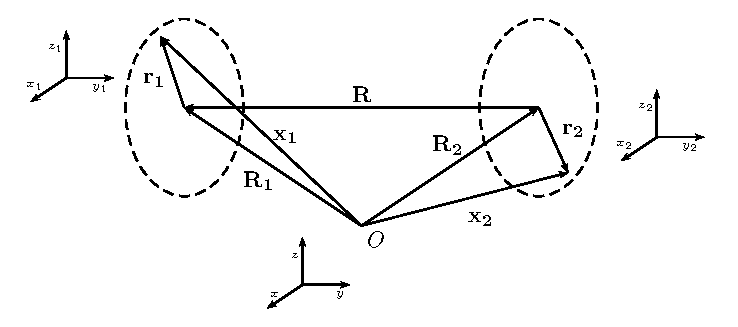
\includegraphics[scale=1.0]{pics/taylor_pspic.eps}
%\input{taylor_pspic}
\caption{The total system is split into subsystems $\mathbf{S_1}$ and $\mathbf{S_2}$.
The $\mathbf{R}_i$ ($i=1,2$)  point to the corresponding  centers of mass (COMs)
with respect to an arbitrary origin $O$. The $\mathbf{x}_i$ as well as the $\mathbf{r}_i$
describe the electron coordinates once with respect to $O$ and once with respect to the COMs.}
\label{taylor_pspic}
\end{figure}

In order to arrive at working expressions we expand the
Coulomb interaction $\hat{V}_{S_1,S_2}$ in powers of $\frac 1R$ obtaining the
asymptotic expansion \cite{santra2002}:

\begin{align}\label{taylor_multi}
\frac{1}{\left| \mathbf{x}_1-\mathbf{x}_2 \right|} = \frac 1R - \frac{\mathbf{\hat{u}}_R \cdot (\mathbf{r}_1-\mathbf{r}_2)}{R^2}
+ \frac{3(\mathbf{\hat{u}}_R \cdot (\mathbf{r}_1-\mathbf{r}_2))^2 - (\mathbf{r}_1-\mathbf{r}_2)^2}{2R^3} + \mathcal{O} \left( \frac 1{R^4} \right)
\end{align}
where $R=|\mathbf{R}| = |\mathbf{R}_1-\mathbf{R}_2|$ is the distance between the COMs
(see Fig.\ref{taylor_pspic}) and $\mathbf{\hat{u}}_R =  \mathbf{R}/|\mathbf{R}|$ is
the unit vector along $\mathbf{R}$. Each of the subsystems has its own coordinate system
residing in the respective center of mass. Such an expansion converges uniformly
if $|\mathbf{r_i}|<R/2$, corresponding to the absence of overlap of electron
densities localized on different subsystems \cite{Ahlrichs76}. We truncate
the series in Eq. (\ref{taylor_multi}) after the third
term and focus on dipole transitions alone. Inserting it into Eq.(\ref{relgolden}) yields
\begin{align}\label{taylor_in}
\Braket{\chi_{\beta,\varepsilon}|\hat{V}_{S_1,S_2}|\Phi} 
          =&  -\frac{3}{R^3} \Braket{\phi_{ov_1}^{(S_1)}|\sum\limits_i \mathbf{r}_1^{(i)}\cdot\mathbf{\hat{u}}_R|\phi_{iv}^{(S_1)}}
           \cdot \Braket{\phi_{0}^{(S_2)}|\sum\limits_j \mathbf{r}_2^{(j)}\cdot\mathbf{\hat{u}}_R|\chi_{ov_2,\varepsilon}^{(S_2)}}
           \nonumber\\
          &+\frac{1}{R^3} \Braket{\phi_{ov_1}^{(S_1)}|\sum\limits_i \mathbf{r}_1^{(i)}|\phi_{iv}^{(S_1)}} \cdot
            \Braket{\phi_{0}^{(S_2)}|\sum\limits_j \mathbf{r}_2^{(j)}|\chi_{ov_2,\varepsilon}^{(S_2)}}
\end{align}
where we made use of the fact that the matrix elements over the first two terms
in the expansion (\ref{taylor_multi}) vanish due to orthogonality of the
decaying and final continuum states. For rewriting Eq.(\ref{taylor_in}) in
spherical coordinates it is convenient to orient $\mathbf{R}$ along the $z_2$ axis leading to
\begin{align}\label{last_matrixelement}
 \braket{\chi_{\beta,\varepsilon}|\hat{V}_{S_1,S_2}|\Phi} 
= \frac{1}{R^3} \sum\limits_{m=0,\pm 1} B_m \braket{\phi_{ov_1}^{(S_1)}|{D}_{1m}|\phi_{iv}^{(S_1)}}  \braket{\phi_{0}^{(S_2)}|{D}_{2m}|\chi_{ov_2,\varepsilon}^{(S_2)}} ,
\end{align}
where $B_0=-2$, $B_{\pm 1}=1$ and $D_{im} = \sum\limits_{i} r_{im}$ ($i=1,2$) are
the dipole operators acting on the electron coordinates of the
subsystems $\mathbf{S_1}$ and $\mathbf{S_2}$, respectively (see \cite{9} for
further details). The general expression for the decay width $\Gamma_\beta$
referring to the decay process then reads as

\begin{align}
\label{sum_squares}
\Gamma_\beta
=  \frac{2\pi}{R^6}\sum\limits_{m=0,\pm 1}B_m^2 \left|
\braket{\phi_{ov_1}^{(S_1)}|{D}_{1m}|\phi_{iv}^{(S_1)}}\right|^2
\left|\braket{\phi_{0}^{(S_2)}|{D}_{2m}|\chi_{ov_2,\varepsilon}^{(S_2)}}\right|^2
\end{align}
and serves as the starting equation for the special cases of ICD and ETMD3
as discussed in the following subsections.

\section{Interatomic Coulombic Decay}
\label{subs_icd}

\begin{figure}[ht]
\centering
\includegraphics[scale=0.30]{pics/ICD_subsystems.eps}
\caption{ICD process in subsystems $\mathbf{S_1}$ and $\mathbf{S_2}$. After
         creating an inner valence vacancy in $\mathbf{S_1}$  the hole is filled
         by an outer-valance electron of $\mathbf{S_1}$. The excess energy is
         transferred to $\mathbf{S_2}$ and is used to remove an outer-valence
         electron (ICD electron).}
\label{fancy_ICD}
\end{figure}

In the ICD process the inner valence vacancy is filled with an electron
of the same atom or molecule. The excess energy is transferred to the secon
subunit and is used to ionize it (see Fig. \ref{fancy_ICD}). In rare gas
clusters the corresponding subunits are atoms leading to the partition
$\mathbf{S_1}$ as atom $A$ and $\mathbf{S_2}$ as atom $B$. In atoms,
the total angular momentum quantum number $J$ and its projection $M$ are
good quantum numbers. As an ansatz for the initial and final state wave
functions under the assumption of no interaction, the product of individual
atomic configuration state functions is taken:
\begin{equation}\label{wf_ansatz}
\ket{\Phi} =\ket{E_A\, J_A\, M_A}\ket{E_B\, J_B\, M_B}
\quad\mbox{and}\quad
\ket{\chi_{\beta,\varepsilon}} = \ket{E'_A\, J'_A\, M'_A}\ket{E'_B\,  J'_B\, M_B'}\, .
\end{equation}
In this expression the initial and final states are characterized by the
energies of the atoms $E_A$, $E_B$ and $E_A'$, $E_B'$, the corresponding
total angular momenta of the atoms are denoted as $J_A$, $J_B$ and
$J_A'$, $J_B'$ and their projections on the $z$-axis as $M_A$, $M_B$ and
$M_A'$, $M_B'$, respectively. At the beginning of the process atom $B$ is
assumed to be in its closed shell ground state $\ket{\Phi_0^{(B)}}$ with
$J_B=M_B=0$. Inserting Eqs. (\ref{wf_ansatz}) into (\ref{sum_squares})
we obtain

\begin{align}
\label{Gamma_ICD_allsum}
\Gamma_\beta =& \frac{2\pi}{R^6} \sum\limits_{m} \, B_{m}^2 \, \left| \braket{E'_A\, J'_A\, M'_A | \hat{D}^{(A)}_{m} | E\, J_A\, M_A}\right|^2 \nonumber\\
        & \times\, \left| \braket{\Phi_0^{(B)} | \hat{D}^{(B)}_{m} | E'_B\, J'_B\, M_B'}^* \right|^2\, \delta (E-E')
\end{align}

At large distances the energies of the decaying and final state can be
assumed to be the sum of the energies of the two subsystems
$A$ and $B$: $E=E_A+E_B$, $E'=E_A'+E_B'$. The resonance condition $E=E'$
can therefore be expressed through the energy matching of virtual photons
emitted in the transition on atom $A$, $\omega_A=E_A-E'_A$, and absorbed
by atom $B$, $\omega_B=E_B'-E_B$, i.e. $\omega_A=\omega_B=\omega_{vp}$.
We can use the conservation of the projection of the angular momentum on
the $z$-axis $M_A=M_A'+M_B'$ to further simplify the expression in
Eq. (\ref{Gamma_ICD_allsum}). By setting $m=-M_B'$ and using the
Wigner-Eckart theorem \cite{EdmondsAngular} we arrive at

\begin{align}\label{reltheolifetime}
 \Gamma_\beta =& \frac{2\pi}{R^6} \sum\limits_{M_A'} \, B_{M_A'-M_A}^2 \, \left| \left(
\begin{array}{ccc}
J_A'  & 1        & J_A\\
-M_A' & M_A'-M_A & M_A
\end{array}\right)
 \braket{E'_A\, J'_A || \hat{D}^{(A)} || E\, J_A}\right|^2 \nonumber\\
        & \times\, \frac 13  \left| \braket{\Phi_0^{(B)} || \hat{D}^{(B)} || E'_B\, J'_B} \right|^2,
\end{align}
where each decay channel $\beta$ is characterized by $E_A'$, $J_A'$, $E_B'$
and $J_B'$.

To find numerical values of $\Gamma_\beta$, the necessary dipole transition
moments of the isolated atoms in Eq. (\ref{reltheolifetime}) can either
be computed directly or obtained from experimentally accessible quantities.
At first we use the fact that the square of the reduced matrix element of
atom $A$, the so-called line strength, is proportional to the state-to-state
transition probability $W_{J_A,J_A'}$, which is in turn the inverse of the
radiative lifetime $\tau$ of the initial state \cite{Sobelman72}:

\begin{equation}
\label{sysa_emission}
  \left| \braket{E'_A\, J'_A || \hat{D}^{(A)} || E\, J_A} \right|^2 = (2J_A +1)\, \frac{3c^3}{4\omega_{vp}^3}\, W_{J_A,J_A'} .
\end{equation}
Second, the square of the reduced matrix element of atom $B$ is related
to its partial  photoionization cross section $\sigma^{(B)}(\omega_{vp})$
which depends on the energy atom $B$ is exposed to \cite{Sobelman72}:

\begin{equation}\label{sysb_absorption}
  \left| \braket{\Phi_0^{(B)} || \hat{D}^{(B)} || E'_{B}\, J'_{B}} \right|^2
   = \frac{3c\,\sigma^{(B)}(\omega_{vp})}{4\pi^2\omega_{vp}} .
\end{equation}
After insertion of Eq.(\ref{sysa_emission}) and (\ref{sysb_absorption})
into (\ref{reltheolifetime}) we arrive at a working expression for the
partial decay width according to

\begin{align}\label{reltheolifetime_exp}
 \Gamma_\beta =& \frac{2\pi}{R^6} \sum\limits_{M_A'} \, B_{M_A'-M_A}^2 \, \left| \left(
\begin{array}{ccc}
J_A'  & 1        & J_A\\
-M_A' & M_A'-M_A & M_A
\end{array}\right) \right|^2
 (2J_A+1)\frac{3c^4 \sigma^{(B)}(\omega_{vp})}{16\pi^2\omega_{vp}^4\tau_A} .
\end{align}
As could be expected from the nonrelativistic formula, the relativistic
expression also shows an $R^{-6}$-behaviour for the energy transfer
corresponding to the interaction of two dipoles.
Setting atomic parameters to their non-relativistic values and summing
over all partial decay widths 
$\Gamma=\sum\limits_\beta \Gamma_\beta$ produces the known
non-relativistic result for the total decay width \cite{Averbukh04,Gokhberg10_1}.

One of our major goals is the inclusion of relativistic effects in the
computation of the decay widths which is achieved by using $J/M_J$ adapted
initial and final state wave functions. As a result, we observe more
energetically distinguishable decay pathways leading to a different energy
distribution of the emitted ICD electrons compared to the nonrelativistic
description. Moreover, if ICD takes place close to its threshold, the number
of open channels might differ in the two cases resulting in different total
ICD rates.

%$$$$$$$$$$$$$$$$$$$$$$$$$$$$$$$$$$$$$$$$$$$$$$$$$$$$$$$$$$$$$$$$$$$$$$$$$$$

\section{Electron Transfer Mediated Decay}
\label{subs_etmd}

\begin{figure}[ht]
\centering
\includegraphics[scale=0.30]{pics/ETMD_subsystems.eps}
\caption{ETMD3 process in subsystems $\mathbf{S_1}$ and $\mathbf{S_2}$ where
         the two atoms A and B participate in the electron transfer and are
         combined to $\mathbf{S_1}$. After inner valence ionization of A,
         the vacancy is filled by an electron from B in $\mathbf{S_1}$.
         The energy is transferred to C ($\mathbf{S_2}$) which is ionized
         and hereby emits the ETMD electron.}
\label{fancy_ETMD}
\end{figure}

In the ETMD3 process (see Fig. \ref{fancy_ETMD}) three atoms are involved
which we denote by $A$, $B$ and $C$. The two subsystems in this case are
$AB$ ($\mathbf{S}_1$) and $C$ ($\mathbf{S}_2$). The initial inner valence
hole is assumed to be located on atom $A$. The electron is transferred
from atom $B$ to atom $A$, while the excess energy is transferred from
$\mathbf{S_1}$ to atom $C$ and used to ionize it. For a convenient
geometric description of the triatomic system undergoing the ETMD3 process
we use Jacobi coordinates as shown in Fig.\ref{etmd_geom_pspic}. All
properties of the $AB$ comprising subsystem $\mathbf{S_1}$ are described in
its local $(\tilde{x}_1, \tilde{y}_1,  \tilde{z}_1)$ coordinate system which
is later backtransformed.

Analog to eq. (\ref{last_matrixelement}) we arrive at

\begin{align}\label{last_matrixelement_etmd}
 \braket{\chi_{\beta,\varepsilon}|\hat{V}_{S_1,S_2}|\Phi} 
=& \frac{1}{R^3} \sum\limits_{ov_1,ov_2,\varepsilon}  \left[
  \braket{\phi_{ov_1}^{(S_1)}|  \begin{pmatrix}
         -\frac{1}{\sqrt{2}}(\tilde{x}_1\cos\alpha- \tilde{z}_1\sin\alpha +i\tilde{y}_1)\\
         \frac{1}{\sqrt{2}}(\tilde{x}_1\cos\alpha- \tilde{z}_1\sin\alpha -i\tilde{y}_1)\\
         -2 (\tilde{x}_1\sin\alpha + \tilde{z}_1\cos\alpha )\\
         \end{pmatrix} |\phi_{iv}^{(S_1)}} \right. \nonumber \\
  & \cdot \left. \braket{\phi_{0}^{(S_2)}| \begin{pmatrix}
                            r_{2+}\\
                            r_{2-}\\
                            r_0\\
                            \end{pmatrix} |\chi_{ov_2,\varepsilon}^{(S_2)}} \right] .
\end{align}

\begin{figure}[ht]
\centering
%\input{coord_etmd_pspic}
\includegraphics[scale=1.00]{pics/coord_etmd_pspic.eps}
\caption{Jacobi coordinates used for the geometric description of the trimer.
        $Q$ is the distance between $A$ and $B$, $R$ the distance from the
        center of mass of $AB$ to $C$ and $\alpha$ the angle between the
        lines represented by $Q$ and $R$.}
\label{etmd_geom_pspic}
\end{figure}

We define the initial state of ETMD as
$\ket{\Phi} = \ket{E_{AB}\,  M_{AB}}\ket{\Phi_0^{(C)}}$ and the final state
as $\ket{\chi_{\beta,\varepsilon}} = \ket{E_{AB}'\, M_{AB}'}\ket{E_C'\,   J_C'\, M_C'}$,
where $E_{AB}$ and $E_{AB}'$, $E_C'$ are the energies of the corresponding
initial and final states of the subsystems. Since the subsystem $AB$ is of
linear symmetry the total angular momentum $J_{AB}$ is no longer a good
quantum number but the projections $M_{AB}$, $M_{AB}'$ still are and serve
for the characterization of $AB$. $J_C'$ is the total angular momentum of $C$
in its final state and $\ket{\Phi_0^{(C)}}$ is the closed shell ground
state of atom $C$ in its initial state. Using Eq. (\ref{sum_squares})
and expressing the electron dipole
moment $\vec{D}_1$ of $\mathbf{S}_1$ in the coordinates
($\tilde{x}_1,\tilde{y}_1,\tilde{z}_1$) we arrive at an intermediate equation
for $\Gamma_\beta$ as

\begin{align} \label{reltheolifetimeetmd}
 \Gamma_\beta =& \frac{2\pi}{R^6} \sum\limits_{M_{AB}'} \left[ 2\left( \left|
                 \braket{M_{AB}'| \tilde{D}_x |M_{AB}} \right|^2 (1+  \cos^2\alpha)
                 + \left|\braket{M_{AB}'| \tilde{D}_z |M_{AB}}\right|^2 \sin^2\alpha \right) \right. \nonumber \\
           & \quad\left.+ 4 \left( \left|\braket{M_{AB}'| \tilde{D}_x |M_{AB}}
             \right|^2\sin^2\alpha
             + \left|\braket{M_{AB}'| \tilde{D}_z |M_{AB}}\right|^2\cos^2\alpha \right)  \right] \nonumber\\ 
           & \times\, \frac 13  \left| \braket{\Phi_0^{(C)} || \hat{D}^{(C)} ||J'_C} \right|^2
         ,
\end{align}
where each decay channel $\beta$ is characterized by its own $E_{AB}'$, $E_C'$
and $J_C'$. The reduced matrix elements of atom $C$ can again be expressed in
terms of its ionization cross section
\begin{equation}\label{mecross}
  \left| \braket{\Phi_0^{(C)} || \hat{D}^{(C)} || E'_{C}\, J'_{C}} \right|^2
   = \frac{3c\,\sigma^{(C)}(\omega_{vp})}{4\pi^2\omega_{vp}} 
\end{equation}
and the transition dipole moments of $AB$ can be conveniently computed
using quantum chemical program packages.
Finally we arrive at the following working equation for the decay
width according to
\begin{align} \label{reltheolifetimeetmd_exp}
 \Gamma_\beta =& \frac{2\pi}{R^6} \sum\limits_{M_{AB}'} \left[ 2\left( \left| \braket{M_{AB}'| \tilde{D}_x |M_{AB}} \right|^2 (1+ \cos^2\alpha) + \left|\braket{M_{AB}'| \tilde{D}_z |M_{AB}}\right|^2 \sin^2\alpha \right) \right. \nonumber \\
           & \quad\left.+ 4 \left( \left|\braket{M_{AB}'| \tilde{D}_x |M_{AB}}\right|^2\sin^2\alpha + \left|\braket{M_{AB}'| \tilde{D}_z |M_{AB}}\right|^2\cos^2\alpha \right)  \right] \nonumber \\ 
           & \times\, \frac{c\sigma^{(C)}(\omega_{vp})}{4\pi^2 \omega_{vp}}
           \delta (\omega_{AB}-\omega_C) .
\end{align}

The corresponding nonrelativistic expression for the ETMD decay width is
obtained by using $L$ and $S$ instead of the total angular momentum $J$ for
each electronic state together with the nonrelativistic virtual photon
energy and the corresponding photoionization cross section. Analogously to
the ICD we observe the $R^{-6}$ behaviour of the energy transfer.
Additionally, an $e^{-\alpha Q}$ dependence is hidden in the transition
dipole moments due to the charge transfer occurring in the ETMD process.




 \chapter{Obtaining Continuum Properties from $\mathcal{L}^2$-Functions}


\section{Bound and Continuum States}
Before we describe the decay of a metastable state, we have to remember,
that both bound and continuum states are involved in such a process.
Bound states are very localized and in quantum mechanics
represented by square integrable
functions of the $\mathcal{L}^2$ Hilbert space. Their boundary conditions
lead to a quantized energy spectrum and the functions of the bound states
are normalized
to represent one particle each. Unperturbed bound states are stationary
and can therefore conveniently be described using the time-independent
Schroedinger equation.
In contrast to the bound states the
continuum states are very delocalized, are not $\mathcal{L}^2$
integrable and are hence not accessible for a probabilistic interpretation.
Their energy spectrum is continuous and the functions are normalized to
their respective energy.

In decay processes
where bound and continuum states interact, it is obliged to find a way to
properly represent bound states in an energy normalization or continuum states
in an $\mathcal{L}^2$ normalization.
Since quantum chemical programme packages are based on $\mathcal{L}^2$ functions,
it is most convenient to go for the latter approach.

After an explanation of Gaussian quadrature we are going to show how
the discrete spectrum of a Hamiltonian in $\mathcal{L}^2$ representation
can be motivated to contain information of the continuum using Gaussian quadrature
based on the discussion of \cite{Reinhardt79}.
Then we are going to show, how the decay width can be obtained from a
discrete pseudo-spectrum by using Stieltjes imaging \cite{Stieltjes}.
Finally we are going to introduce the FanoADC approach for the creation of
states in the $\mathcal{L^2}$ \ac{ISR} basis.



\section{Gaussian Quadrature}
The gaussian quadrature is a numerical method for integration. By approximating
the function to be integrated $g(x) = \rho(x) f(x)$ to be a product of a
positive definite weight
function $\rho (x)$ and a continuous and bounded function $f(x)$.

The evaluation of the integral is then desired to be obtained as

\begin{equation}
  \int\limits_a^b \rho(x) f(x) dx \approx \sum\limits_{i=1}^n \omega_i f(x_i)
\end{equation}

, where the weigths $\omega_i$ and the abcissae $x_i$ are to be determined
analytically, if possible, or otherwise in an optimal way. This leads the abcissae
to be unequally spaced unlike in the basic
integration schemes using the trapezoidal rule.

The function $f(x)$ can be expressed as a polynomial.
For certain weight functions and boundaries
of integration, these
polynomials can be determined analytically.
It can furthermore be shown, that the roots (zeros) of the highest order polynomial
describing $f(x)$ give the optimal abcissae $x_i$.

In case of
$\omega(x)= \frac{1}{\sqrt{1-x^2}}$ and the condition

\begin{equation}
  \int\limits_{-1}^{1} \rho(x) Q_n(x) Q_m(x) = N_n \delta_{nm}
\end{equation}

, where $N_n$ denotes the normalization factor,
the solution to the polynomials are the so-called Chebyshev polynomials, with

\begin{equation}
  x_{i,n} = \cos \left( \frac{2i-1}{2n} \pi \right)
  \quad\quad \omega_{i,n} = \frac \pi n .
\end{equation}

\begin{figure}[ht]
  \centering
  \begin{tikzpicture}
    \begin{axis}[%scale=0.8,
                 domain=-1.0:1.0,
                 samples = 200,
                 %xtick={-3.14159,-1.57089,...,3.14159},
                 %xticklabels={$-\pi$,$-\frac \pi 2$,0,$\frac \pi 2$,$\pi$},
                 cycle list name = exotic,
                 %legend style={anchor= north west},
                 legend pos = north west,
                 legend cell align = left,
                 reverse legend
                 ]
     \addplot+[domain=-1:-0.965925826289+0.135517335117/2,
              diplom1,
              mark = none,
              %forget plot,
              pattern = north east lines,
              pattern color = diplom1
              ]
              {0.0987789349866} \closedcycle;
     \addlegendentry{approximation}
     \addplot+[domain=-0.965925826289+0.135517335117/2:-0.707106781187+0.370240244847/2,
              diplom1,
              mark = none,
              forget plot,
              pattern = north east lines,
              pattern color = diplom1
              ]
              {0.646446609407} \closedcycle;
     \addplot+[domain=-0.707106781187+0.370240244847/2:-0.258819045103+0.505757579964/2,
              diplom1,
              mark = none,
              forget plot,
              pattern = north east lines,
              pattern color = diplom1
              ]
              {0.982662411472} \closedcycle;
     \addplot+[domain=-0.258819045103+0.505757579964/2:0.258819045103+0.505757579964/2,
              diplom1,
              mark = none,
              forget plot,
              pattern = north east lines,
              pattern color = diplom1
              ]
              {1.017337588535} \closedcycle;
     \addplot+[domain=0.258819045103+0.505757579964/2:0.708718898022+0.370240244847/2,
              diplom1,
              mark = none,
              forget plot,
              pattern = north east lines,
              pattern color = diplom1
              ]
              {1.353553390592} \closedcycle;
     \addplot+[domain=0.708718898022+0.370240244847/2:1.0,
              diplom1,
              mark = none,
              forget plot,
              pattern = north east lines,
              pattern color = diplom1
              ]
              {1.901221065013} \closedcycle;
     \addplot [only marks,mark=o,thick]
       coordinates {
                   ( 0.965925826289, 1.901221065013 )
                   ( 0.707106781187, 1.353553390592 )
                   ( 0.258819045103, 1.017337588535 )
                   (-0.258819045103, 0.982662411472 )
                   (-0.707106781187, 0.646446609407 )
                   (-0.965925826289, 0.0987789349866)
                   };
     \addlegendentry{$h_i(x_i)$}
     \addplot [diplom2, thick]
              {x^3 + 1};
     \addlegendentry{$h(x)= x^3 + 1$}
    \end{axis}
\end{tikzpicture}

  \caption{Integration by Gauss-Chebyshev quadrature of the function
           $f(x)=x^3 + 1$ (dark blue) with $n=6$. The integral (light blue)
           is approximately obtained by summation
           over all product of optimal abcissae and weights $x_if(x_i)$ (circles).}
  \label{figure:gaussian_quadrature}
\end{figure}

This means, that the integration of an arbitrary function $h(x)$ within
the interval $[-1,1]$ can be integrated as

\begin{equation}
  \int\limits_{-1}^1 h(x) dx = \int\limits_{-1}^1 \omega(x) \sqrt{1-x^2} h(x) dx
  \approx \frac \pi n \sum\limits_{i_1}^n h(x_i) \sqrt{1-x_i^2}
\end{equation}

An example for such an integration is shown in figure \ref{figure:gaussian_quadrature}
for $h(x) = x^3 + 1$. The dark blue curve shows $h(x)$, the points are the
calculated $f_i$ at the abcissae $x_i$ and the light blue hatched areas are the
approximations to the integral for the certain areas.

For an unknown weight function, the integral can be obtained by solving the so-called
moment problem.




\section{Expressing the Continuum Properties in Terms of Gaussian Quadrature}
The Hamiltonian can be expressed in terms of a complete set of eigenfunctions

\begin{equation} \label{equation:complete_hamniltonian}
  H = \sum\limits_i \ket{\phi_i} E_i \bra{\phi_i}
     + \int\limits_0^\infty \mathrm{d}E \ket{\phi(E)} E \bra{\phi(E)}  ,
\end{equation}
where the manifold of $\phi_i$ denote the bound state eigenfunctions being orthonormal
in the sense of the probabilistic picture $\braket{\phi_j|\phi_i} = \delta_{ij}$.
The continuum functions $\phi(E)$ also form an orthonormal set of basis functions
but are normalized with respect to their energy.

\begin{equation}
  \braket{\phi(E) | \phi(E')} = \delta(E-E')
\end{equation}

In a calculation using a finite $\mathcal{L}^2$ basis, the diagonalization of the
Hamiltonian yields an approximative set of eigenfunctions $\chi_i$ with corresponding
eigenvalues $\tilde{E}_i$ such that

\begin{equation}
  \tilde{H} \ket{\chi_i} = \tilde{E}_i \ket{\chi_i} \quad\quad  \,
  \braket{\chi_j|\chi_i} = \delta_{ij} .
\end{equation}

If we now rewrite the approximative Hamiltonian in terms of these $\mathcal{L}^2$
functions, we obtain

\begin{equation}
  \tilde{H} = \sum\limits_{E_i<0} \ket{\chi_i} \tilde{E}_i \bra{\chi_i}
            + \sum\limits_{E_j>0} \ket{\chi_j} \tilde{E}_j \bra{\chi_j}   ,
\end{equation}
where the first part with eigenvalues smaller than 0 corresponding to the
bound states and the second part with energies higher than 0 containing to
the continuum. In this representation the continuum is not described explicitely,
but in a discretized representation.

The eigenfunctions and eigenvalues of the positive energy solutions have no physical
meaning, because for more and more complete bases, the energies will approach zero
and the eigenfunctions will be arbitrarily diffuse. Still, they inhibit a useful
mathematical meaning if the continuum part is interpreted in terms of
a numerical quadrature.
In the case of integrating the continuum part of equation
\ref{equation:complete_hamniltonian} for evaluation of the energy expectation
value $\braket{\Psi| H | \Psi}$
with first gaussian quadrature and second the discrete positive energy
eigenfunctions, the continuum part of the expectation value reads as


\begin{align}
  \int\limits_0^\infty \mathrm{d}E \braket{\Psi|\phi(E)} E \braket{\phi(E)|\Psi}
  &\simeq \sum\limits_j \omega_j \braket{\Psi|\phi(E_j)} E_j \braket{\phi(E_j)|\Psi}
\end{align}



\begin{equation}
  \int\limits_0^\infty \mathrm{d}E \braket{\Psi|\phi(E)} E \braket{\phi(E)|\Psi}
  \simeq \sum\limits_{E_j}  \braket{\Psi|\chi} \tilde{E}_j \braket{\chi|\Psi}   .
\end{equation}

In both cases, the integral is approximated by a sum and in some special cases, where
the analytic continuum functions are known, it can be shown from the results,
that there seems to be a one-to-one corespondence between each $\mathcal{L}^2$
eigenfunction of the positive energy part and the continuum function evaluated
at the energy $\tilde{E}_j$. The equivalent quadrature weight connects the discrete and
the continuum function for the given energy and acts by renormalization.

\begin{equation}
  \ket{\chi_j} = \sqrt{\omega_j^{Eq}} \ket{\phi(\tilde{E}_j)}
\end{equation}

In the following, we are going to assume, that this equivalence between $\mathcal{L}^2$
and continuum functions with the integral interpreted as Gaussian quadrature
is true for all our systems under investigation.

If we for a moment assume, that we knew the appropriate equivalent quadrature
weigths, we could calculate the decay width from a continuous representation as

\begin{equation}
  \Gamma = \frac 1{\omega_{j}^{Eq}} \left| \braket{\Phi_s|H-E|\chi_j} \right|^2
\end{equation}

Since unfortunately in most cases, the weigth function is unknown, we are going
to calculate the weigth function by solving the moment problem, since the moments

\begin{equation}
  \Gamma^k = 2\pi \sum\limits_i \left| \braket{ \Psi | H-E | \chi_i } \right| ^2
\end{equation}
of the discrete representation are well defined and accessible,
with $\Psi$ being the wave function of the initial state.



\subsection{Moment Problem}

The moments $S(k)$ of a real and continuous function $f(\omega)$ are defined
as

\begin{equation}
  S(k) = \int\limits_a^b \omega^k f(\omega) d\omega \quad\quad k=0,1,\dots  .
\end{equation}

In case of $f(\omega)$ being a probability density function, it is connected
to the probability distribution function $F(\omega)$ via
\begin{equation}
  F(\omega) = f(\omega){d\omega} .
\end{equation}

The probability density function is completely determined by the manifold
of moments. Therefore, when all moments are known, the probability density
function  (weight function) can be calculated from the moments.
In the present case $f(\omega)$
is the decay width $\Gamma(E)$, but the theory is also applicable and very often
used for the description of cross sections. Its pseudo-spectrum has the same
mathematical properties as the pseuso-spectrum of the decay width. Therefore,
the knowledge obtained in the description of cross sections can be adopted to
the description for the decay widths.

In practice, all moments are never available unless the moments can be
calculated analytically. Therefore, one has to approximately solve the reduced
moment problem, since the density function is not completely defined.
In this case the $2r$ moments are

\begin{equation}
  S(k) = \int\limits_a^b \omega^k f(\omega) d\omega \quad\quad k=0,1,...,2r-1
\end{equation}

In principle the moment problem can be solved by requiring the abscissae and
weights to reproduce a minimum number of moment. Unfortunately, this determination
is ill conditioned and therfore, one expresses the moments by orthogonal
polynomials of some known weight function. In this case, then the
transformation to the polynomials is ill conditioned, but the abscissae
and weights can be obtained by a well conditioned problem. The latter approach
of so-called modeified moments has shown to be useful in the case of
properties such as the ionization
cross section and decay width.





\subsection{Finding the Gaussian Quadrature Abscissae and Weights from Modified Moments}

The procedure for the calculation of cross sections combining moment
theory and Gaussian quadrature has been investigated thoroughly. In this section
we follow the argumentation of Müller-Plathe \cite{}, from which the
\verb|stieltjes| routine has been written by Averbukh and which is used in
combination with the FanoADC implemented in Dirac.

For the ionization cross sections it has been shown, that the moment with
$k>2$ diverge and hence are useless for the evaluation of the probability
density function $f(\omega)$. Therefore the inverse moment $S(-k)$ are investigated
instead.

\begin{equation}
  S(-k) = \int\limits_a^b \left( \frac{1}{\omega} \right) ^k f(\omega) d\omega
\end{equation}

For each \emph{order of Stieltjes} $r$, a set of
Chebyshev polynomials
$Q_n (1/\omega) = \sum\limits_{i=0}^n Q_n^{i}\left( \frac{1}{\omega} \right)^{i}$,
of order $0-r$ can be assigned, using $2r-1$ moments.
They are orthogonal with respect to the weight function
to be determined $f(\omega)$.

\begin{equation}
  \int\limits_a^b Q_n(1/\omega) \, Q_m(1/\omega) f(\omega) d\omega = N_n \delta_{nm}
\end{equation}

They are normalized such, that the coefficient of the highest power polynomial
equals 1.

\begin{equation}
  N_n = \int\limits_a^b \left[ Q_n(1/\omega) \right]^2 f(\omega) d\omega
\end{equation}

Chebyshev polynomials in general can be constructed from an recursion formula
\begin{equation}
  Q_n(1/\omega) = \frac{1}{\omega - a_n} Q_{n-1}(1/\omega) - b_{n-1} Q_{n-2}(1/\omega)
\end{equation}

, so that all polynomials can be constructed if $Q_0$ and $Q_1$ are known.
From these recursion relations, expressions for the recursion coefficients
$a_n$ and $b_n$ can be obtained.

\begin{align}
  a_n     &= \frac{1}{b_0b_1\cdots b_{n-1}}
             \int (1/\omega)^n Q_{n-1}(1/\omega) f(\omega) d\omega
             - \sum\limits_{l=1}^{n-1} a_l  \label{equation:an_cont}\\
  b_{n-1} &= \frac{1}{b_0b_1\cdots b_{n-2}}
             \int (1/\omega)^{n-1} Q_{n-1}(1/\omega) f(\omega) d\omega \label{equation:bn_cont}
\end{align}

By expansion of the integral in equations \ref{equation:an_cont} and
\ref{equation:bn_cont} into a sum over moments obtained from the pseudo-spectra,
approximate expressions can be obtained for the recursion coefficients
depending on the energies $\bar{\omega}_i$, here the inverse abcissae,
and decay widths or the weights $\bar{f}_i$ of the
pseudo-spectrum.

\begin{align}
  a_n     &= \frac{1}{b_0b_1\cdots b_{n-1}}
             \sum\limits_{i=1}^N
               (1/\bar{\omega}_i)^n Q_{n-1}(1/\bar{\omega_i}) \bar{f}_i
             - \sum\limits_{l=1}^{n-1} a_l \label{equation:an_disc}\\
  b_{n-1} &= \frac{1}{b_0b_1\cdots b_{n-2}}
             \sum\limits_{i=1}^N
               (1/\bar{\omega}_i)^{n-1} Q_{n-1}(1/\bar{\omega}_i) \bar{f}_i
\end{align}

Hence the recursion relation now reads as
\begin{equation}
  Q_n(1/\bar{\omega}_i) = \frac{1}{\bar{\omega}_i - a_n} Q_{n-1}(1/\bar{\omega}_i)
                          - b_{n-1} Q_{n-2}(1/\bar{\omega}_i)
\end{equation}

with
\begin{equation}
  Q_0(1/\bar{\omega}_i) = 1 \quad\quad Q_1(1/\bar{\omega}_i) = (1/\bar{\omega}_i) - a_1
\end{equation}
as starting points of the determination of the polynomials.

As discussed above in section \ref{section:}, given the weights, the polynomials
can be calculated. In the Stieltjes imaging, starting from the polynomials
defined by the discrete pseudo-spectrum, one wants to achieve the weight function.
Also here the ideal abscissae are the roots of the highest order polynomial
for each moment $k$

\begin{equation}
  Q_n(1/\omega_i) = 0 \quad\quad i = 1,2,\dots ,n .
\end{equation}

The connection between the weights with the polynomials is given by

\begin{equation}
  f_i = \left[ \sum\limits_{m=0}^{n-1} \frac{Q_m^2(1/\omega_i)}{N_m} \right]^{-1} .
\end{equation}

In order to obtain the roots of the highest order polynomial, in principle
any programm for root detection can be used. However, the problem can
be reformulated in the means of general polynomials $R_n(1/\omega)$ connected
to the obtained Chebyshev polynomials
\begin{equation}
  Q_n(1/\omega) = (-1)^n \sqrt{N_n} R_n(1/\omega)
\end{equation}

with the recursion formulas
\begin{equation}
  (1/\omega)R_{n-1}(1/\omega) = - \sqrt{b_n}R_n(1/\omega) + a_nR_{n-1}(1/\omega)
                                - \sqrt{b_{n-1}} R_{n-2}(1/\omega)
\end{equation}
and
\begin{equation}
  (1/\omega)R_0(1/\omega) = - \sqrt{b_1}R_1(1/\omega) + a_1 R_0(1/\omega) .
\end{equation}

Now the roots can be determined of the following equation disregarding the
last vector by solving the eigenvalue problem.

\begin{equation}
 \begin{split}
 \begin{pmatrix}
a_1        & -\sqrt{b_1}&            &                &             &          \\
-\sqrt{b_1}& a_2        & -\sqrt{b_2}&                &             &          \\
           & -\sqrt{b_2}& a_3        & -\sqrt{b_3}    &             &          \\
           &            & \ddots     & \ddots         & \ddots      &          \\
           &            &            & -\sqrt{b_{n-2}}& a_{n-1}     & -\sqrt{b_{n-1}}\\
           &            &            &                & -\sqrt{b_{n-1}}& a_n   
 \end{pmatrix}
 \begin{pmatrix}
  R_0(1/\omega)\\
  R_1(1/\omega)\\
  R_2(1/\omega)\\
  \vdots\\
  R_{n-2}(1/\omega)\\
  R_{n-1}(1/\omega)
 \end{pmatrix}         \\
 = (1/\omega)
 \begin{pmatrix}
  R_0(1/\omega)\\
  R_1(1/\omega)\\
  R_2(1/\omega)\\
  \vdots\\
  R_{n-2}(1/\omega)\\
  R_{n-1}(1/\omega)
 \end{pmatrix}
 -
 \begin{pmatrix}
  0\\
  0\\
  0\\
  \vdots\\
  0\\
  -\sqrt{b_n} R_{n}(1/\omega)
 \end{pmatrix}
 \end{split}
\end{equation}

Therefore the solution is simplyfied to a matrix diagonalization
of the coefficients matrix. Its eigenvalues are the roots of the polynomial
and hence the wanted abcissae. The eigenfunctions are normalized to 1 and therefore
have to be renormalized according to

\begin{equation}
  1 = f_i \sum\limits_{m=0}^{n-1} R_m^2 (1/\omega_i) = \mathbf{u_i} \cdot \mathbf{u_i}
\end{equation}
from equation \ref{} to give

\begin{equation}
  f_i = N_0 u_{0i}^2
\end{equation}

for the weights.

\begin{equation}
  S(-k) = \sum\limits_{i=1}^n f_i (1/\omega_i)^k \quad\quad k=0,1,\dots,2n-1
\end{equation}





\subsection{Stieltjes Imaging}
Having obtained the abcissae and weights, the probability distribution function
$F(\omega)$ can be approximated. For this purpose the so-called Stieltjes imaging
is employed, where

\begin{equation}
  F^{(n)} (\omega) =
  \begin{cases}
    0                                & \omega < \omega_1\\
    \sum\limits_{j=1}^{i} f_j        & \omega_i < \omega < \omega_{i+1}\\
    \sum\limits_{j=1}^{i} f_j = S(0) & \omega_n < \omega 
  \end{cases}
\end{equation}
which is illustrated in figure \ref{figure:stieltjes_imaging} for a sixth
order stieltjes procedure using a pseudo-spectrum for the NeAr ICD in a
Stieltjes histogram.


\begin{figure}[h]
  \centering
  %NeAr at 3.42 AA, 6th order of stieltjes
\begin{tikzpicture}
    \begin{axis}[%scale=0.8,
                 domain=-1.0:1.0,
                 samples = 200,
                 %xtick={-3.14159,-1.57089,...,3.14159},
                 %xticklabels={$-\pi$,$-\frac \pi 2$,0,$\frac \pi 2$,$\pi$},
                 cycle list name = exotic,
                 legend style={anchor= north west},
                 legend cell align = left,
                 xlabel= {$E$ [a.u.]},
                 ylabel= {$F(E)$}
                 ]
     \addplot+[domain=-1:-0.42789448546292908,
              diplom1,
              mark = none,
%              forget plot,
              pattern = north east lines,
              pattern color = diplom1
              ]
              {0.0} \closedcycle;
     \addlegendentry{$\sum\limits_{j=1}^{i} f_j \quad \omega_i < \omega < \omega_{i+1}$}
     \addlegendimage{empty legend}
     \addlegendentry{}
     \addplot+[domain=-0.42789448546292908:-0.25969072398345394,
              diplom1,
              mark = none,
              forget plot,
              pattern = north east lines,
              pattern color = diplom1
              ]
              {0.000790314507333} \closedcycle;
     \addplot+[domain=-0.25969072398345394:0.11385089684626037,
              diplom1,
              mark = none,
              forget plot,
              pattern = north east lines,
              pattern color = diplom1
              ]
              {0.00156501308103} \closedcycle;
     \addplot+[domain=0.11385089684626037:1.4305018410002852,
              diplom1,
              mark = none,
              forget plot,
              pattern = north east lines,
              pattern color = diplom1
              ]
              {0.00208878898366} \closedcycle;
     \addplot+[domain=1.4305018410002852:5.1882229137192883,
              diplom1,
              mark = none,
              forget plot,
              pattern = north east lines,
              pattern color = diplom1
              ]
              {0.0022929712885} \closedcycle;
     \addplot+[domain=5.1882229137192883:6,
              diplom1,
              mark = none,
              forget plot,
              pattern = north east lines,
              pattern color = diplom1
              ]
              {0.00241086375443} \closedcycle;
%     \addplot [diplom2, thick,
%               domain=-0.5:6]
%              %{0.001300 * ln(x+2.594992)};
%              {0.001049 * sqrt(x+1.374436)};
%     \addlegendentry{$F(x)= \frac 13 x^3 + x^2 + 2x$}
     \addplot [samples=200,mark=*,thick,smooth,diplom2]
       coordinates {
                   (-0.42789448546292908, 0.0003951572536665)
                   (-0.25969072398345394, 0.0011776637941815)
                   ( 0.11385089684626037, 0.001826901032345)
                   ( 1.4305018410002852, 0.00219088013608)
                   ( 5.1882229137192883, 0.002351917521465)
                   };
     \addlegendentry{$\approx F(E_i)$}
    \end{axis}
\end{tikzpicture}

  \caption{Stieltjes histogram of a sixth order integration from
           an NeAr ICD pseudo-spectrum (light blue). At the abcissae $\omega_i$,
           the histogram provides lower and upper bounds for the actual
           values. The mean of these two bounds (dark blue) normally is a good
           approximation of the distribution function $F(E)$ at this point.}
  \label{figure:stieltjes_imaging}
\end{figure}

This procedure is based on the so-called Chebyshev inequalities

\begin{equation} \label{equation:Chebyshev_inequalities}
  F^{(n)}(\omega_i - 0) \le F^{(n+1)}(\omega_i - 0) \le F(\omega_i)
  \le F^{(n+1)}(\omega_i + 0) \le F^{(n)}(\omega_i + 0).
\end{equation}

This means, that the distribution functions obtained from the Chebyshev
polynomials approaching the abcissae $\omega_i$ from below and above
give lower and upper bounds to the actual value of the distribution
function at this particular point $F(\omega_i)$. In fact, the mean of these
two values normally is a very good approximation to the exact value.

\begin{equation}
  F^{(n)} (\omega_i) = \frac 12 \left[ F^{(n)} (\omega_i - 0)
                       + F^{(n)} (\omega_i+0) \right]
\end{equation}

Since we evaluated the integral,
which was the equaling quantity for both the Gaussian quadrature ansatz
in equation \ref{equation:} and the discrete spectrum in equation
\ref{equation:}, the distribution function obtained from the
discrete pseudo-spectrum is normalized correctly.
This distribution function is then numerically differenciated via

\begin{equation}
  f^{(n)} (\omega) =
  \begin{cases}
    \frac 12 \frac{f_1}{\omega_1}    & \omega < \omega_1\\
    \frac 12 \frac{f_{i+1} + f_i}{\omega_{i+1} - \omega_i}
                                     & \omega_i < \omega < \omega_{i+1}\\
    0                                & \omega_n < \omega
  \end{cases}
\end{equation}

to give  $r-1$ non-zero points of the desired
density function $f(\omega)$, which are
subsequently interpolated. In the routine of Averbukh, a spline interpolation
is used for this purpose. Afterwards the interpolated density function is evaluated
for the energy of interest, which is the resonance energy $E_r$ in case of the
autoionization processes.

\subsection{Quality and Stability of the Results}
The abcissae of the polynomials constructed from different orders
of moments intersect each other as is schematically shown in
figure \ref{figure:stieltjes_density}, where each colour of points corresponds
to one order. Therefore, in an ideal world, where all these points exactly lie
on the desired desity function, the combination of all abscissae
and weights for the interpolation is beneficial.

\begin{figure}[h]
  \centering
   \begin{tikzpicture}[
          scale=1.0,>=stealth,domain=0.5:8,samples=100,
          declare function={
          xshift = 0.7;
          yshift = 0.3;
          gamma(\x) = 1.5/(\x+xshift)^2  +yshift;
          noise(\x) = 1.5*exp(-1.0*(\x+xshift))*cos(10*(\x+xshift) r);
          calcgamma(\x) = gamma(\x) + noise(\x);
        }]
     \small
%  \draw[very thin,color=gray] (-0.1,-0.1) grid (4.9,4.9);
  \draw[->,thick] (-0.2,0) -- (5.2,0) node[right] {$E$};
  \draw[->,thick] (0,-0.2) -- (0,4.2) node[above] {$\Gamma(E)$};
  % add ticks
  \draw [thick] (4,0) -- (4,-2pt) node [anchor=north] {$E_r$};
  \draw [color=black,domain=0:5,smooth,very thick]    plot
         (\x,{gamma(\x)}) node [anchor=south east] {density function};
  \foreach \x in {0.2,0.8,...,5}
    \fill[color=orange!80] (\x,{gamma(\x)}) circle (0.08);
  \foreach \x in {0.4,1.0,...,5}
    \fill[color=diplom1!80] (\x,{gamma(\x)}) circle (0.08);
  \foreach \x in {0.6,1.2,...,5}
    \fill[color=diplom2!80] (\x,{gamma(\x)}) circle (0.08);
%  \draw [color=red,domain=0.0:5,smooth,thick]    plot
%         (\x,{calcgamma(\x)}) node [above left=20pt] {real life};
 \end{tikzpicture}
 \begin{tikzpicture}[
          scale=1.0,>=stealth,domain=0.5:8,samples=100,
          declare function={
          xshift = 0.7;
          yshift = 0.3;
          gamma(\x) = 1.5/(\x+xshift)^2  +yshift;
          noise(\x) = 1.5*exp(-1.0*(\x+xshift))*cos(10*(\x+xshift) r);
          calcgamma(\x) = gamma(\x) + noise(\x);
        }]
     \small
%  \draw[very thin,color=gray] (-0.1,-0.1) grid (4.9,4.9);
  \draw[->,thick] (-0.2,0) -- (5.2,0) node[right] {$E$};
  \draw[->,thick] (0,-0.2) -- (0,4.2) node[above] {$\Gamma(E)$};
  % add ticks
  \draw [thick] (4,0) -- (4,-2pt) node [anchor=north] {$E_r$};
  \draw [color=black,domain=0:5,smooth,very thick]    plot
         (\x,{gamma(\x)}) node [anchor=south east] {density function};
%  \foreach \x in {0.2,0.8,...,5}
%    \fill[color=orange!80] (\x,{gamma(\x)}) circle (0.08);
%  \foreach \x in {0.4,1.0,...,5}
%    \fill[color=diplom1!80] (\x,{gamma(\x)}) circle (0.08);
%  \foreach \x in {0.6,1.2,...,5}
%    \fill[color=diplom2!80] (\x,{gamma(\x)}) circle (0.08);
  \draw [color=red,domain=0.0:5,smooth,thick]    plot
         (\x,{calcgamma(\x)}) node [above left=20pt] {real life};
 \end{tikzpicture}

  \caption{Schematic illustration of the interpolation after the
           stieltjes calculations to yield the density function $\Gamma(E)$,
           which is to be evaluated at the resonance energy $E_r$.
           Suppose the black curve to be the
           exact result. Then (left panel), for each order of Stieltjes calculation
           the points lie on this curve, where points from different orders
           (different colours of the points) intersect each other. The interpolation
           gives the exact result. In reality (right panel) the
           interpolations (even of each moment)
           are likely to show oscillations due to non-orthogonalities of
           Chebyshev polynomials in the higher orders and inaccurate descriptions
           due to a large gap between the lower and upper bounds for low
           orders.}
  \label{figure:stieltjes_density}
\end{figure}

As can be seen from the Chebyshev inequalities in
equation \ref{equation:Chebyshev_inequalities}, the higher the highest
power of the polynomials and hence the larger the degrees of freedom are,
the closer the lower and upper bounds get to the exact result.

Unfortunately, the moment problem is ill-conditioned and by introducing
the polynomials, the moment problem as such get well-conditioned but instead
the construction of the polynomials from the pseudo-spectrum is ill-conditioned.
As can be seen from the Chebyshev inequalities, one would like to go to as
high orders as possible, to get more accurate results. But in the construction
of the recursion coefficients \ref{equation:an_disc}, two very large numbers
are subtracted from each other. This is known to be numerically instable.
And the higher the order of the moment is, the bigger
are these numbers and hence the introduced error. Therefore the number
of moments to be successfully employed for the approximation of the
density function is limited by the quality of the orthogonality of
the corresponding set of constructed polynomials. In the final density function
non-orthogonalities as well as errors from inaccurate descriptions of lower
orders can be detected by the presence of oscillations as shown in
figure \ref{figure:stieltjes_density} in the right panel. In case of the density
function being well behaved in the area of the resonance energy $E_r$, the
description might still be feasible. In case of strong oscillations, the validity
of the results are highly questionable. The interpolation can be smoothed
by taking only stable orders of stieltjes into account or in other words
reduce the allowed threshold of allowed non-orthogonality or to give points
stemming from lower orders of Stieltjes higher weights in the interpolation.

\section{Description of Interactions of Bound and Continuum States}
 \chapter{Algebraic Diagrammatic Construction (ADC)}

The \ac{ADC} is a Green's function approach for the calculation of ionization
nergies and electron affinities.
Its advantage is the ability to determine the desired ionization energies
without explicit calculation of the initial and final states, but instead
obtaining their energy differences directly.

Originally, the Green's function was formulated in the Dyson ansatz and
determined using perturbation theory. This way both the ionization and the
electron affinity part had to be included in the description. In the non-Dyson
scheme those two are separable and hence the dimension of the problem is reduced
when one is interested in either the $N+1$ or the $N-1$ part \cite{Schirmer98}.

\begin{equation}
 G_{pq}(\omega) = G^+_{pq}(\omega) + G^-_{pq}(\omega)
\end{equation}

The ionization part $\mathbf{G^-}(\omega)$ is transposed to give
$\tilde{G}_{pq}(\omega) = G^-_{qp}(\omega)$. From this, the compact matrix
form can be deduced

\begin{equation}\label{matrixspec}
\mathbf{\tilde{G}}(\omega) = \mathbf{x}^\dagger(\omega-\mathbf{\Omega})^{-1}\mathbf{x}
\end{equation}

To this point, the approach is exact. However, the exact wavefunctions are unknown
and hence the basis of so-called \emph{intermediate states} is introduced. These
are formally constructed from \ac{CES} as they appear in a
\ac{CI} expansion. These \ac{CES} are then grouped into excitation classes
and these classes are orthogonalized with respect to each other. Afterwards,
the states within each class are orthogonalized. 
This approach has the advantage to be size-consistent and hence
suiTable for the description of larger systems. \cite{Mertins96_1}

In this \ac{ISR} the Green's function can be written as
\begin{equation}\label{isradc}
\mathbf{\tilde{G}}(\omega) = \mathbf{f}^\dagger(\omega-\mathbf{M})^{-1}\mathbf{f}
\end{equation}

with the Hamiltonian $\mathbf{M}$.
This equation can be solved by
considering the eigenvalue problem

\begin{equation}\label{adcewp}
(\mathbf{K}+\mathbf{C}) \mathbf{Y} = \mathbf{Y}\mathbf{\Omega} \quad\text{where } \mathbf{Y}^\dagger\mathbf{Y}=\mathbf{1}
\end{equation}
where $\mathbf{\Omega}$ is the matrix of eigenvalues and hence the ionization
energies and $\mathbf{Y}$ is the matrix of eigenvectors which connects the
intermediate state representation with the exact $N-1$ solutions.

\begin{equation}
 \mathbf{x} = \mathbf{Y}^\dagger \mathbf{f}
\end{equation}

For the construction of the \ac{ADC} matrix $\mathbf{M}$ and the
effective transitions moments $\mathbf{f}$, $\mathbf{M}$ and $\mathbf{f}$
are expanded into different orders of perturbations and inserted to equation
(\ref{isradc}).

\begin{eqnarray}
\mathbf{M} &=& \mathbf{M}^{(0)} + \mathbf{M}^{(1)} + \mathbf{M}^{(2)} + \cdots\label{stf}\\
\mathbf{f} &=& \mathbf{f}^{(0)} + \mathbf{f}^{(1)} + \mathbf{f}^{(2)} + \cdots\label{stf}
\end{eqnarray}

From this, different orders of perturbation theory of the Hamiltonian can be
constructed successively. Hereby, the truncation after the $n$-th order leads
to ADC($n$). The contributions to the different classes for different
orders of \ac{ADC} are shown
in Figure \ref{figure:adcmat_pgf}.

\begin{figure}[h]
  \centering
  \begin{tikzpicture}[scale=1.3]
    \footnotesize
    %\draw [help lines] (-1,0) grid (23,5);
    \draw [thick] (0,0) rectangle (3,3);
    \draw [thick] (0,2) rectangle (1,3) node [midway] {0,1,2,2,3};
    \draw [thick] (1,0) rectangle (3,2) node [midway] {--,--,0,1,1};
    \draw [thick] (0,0) rectangle (1,2) node [midway] {--,--,1,1,2};
    \draw [thick] (1,2) rectangle (3,3) node [midway] {--,--,1,1,2};
    \node (1h1) at (0.5,3.5) {1h};
    \node (1h2) at (-0.5,2.5) {1h};
    \node (2h1) at (2.0,3.5) {2h1p};
    \node (2h2) at (-0.5,1.0) {2h1p};

\end{tikzpicture}

  \caption{Schematic illustration of an \ac{ADC}($n$) matrix for different orders
           of perturbation for $n=0,1,2,2x,3$. ADC(2x) is an extended ADC(2)
           including first
           order contributions to the satellite block.}
  \label{figure:adcmat_pgf}
\end{figure}

The matrix elements of ADC(2x) are explicitely given by
\begin{itemize}
 \item 1h/1h (1h block):
   \begin{align}
    M_{kk'}^{(0)} &= \varepsilon_k \delta_{kk'} \\
    M_{kk'}^{(1)} &= 0 \\
    M_{kk'}^{(2)} &= -\frac12 \sum\limits_{abl} V_{ab[kl]} V_{k'l[ab]} %\times
                     \frac{\varepsilon_a+\varepsilon_b-\varepsilon_l
                       -\frac12 \varepsilon_k-\frac12 \varepsilon_{k'}}
                     {(\varepsilon_a+\varepsilon_b-\varepsilon_k-\varepsilon_l)
                      (\varepsilon_a+\varepsilon_b-\varepsilon_{k'}-\varepsilon_l)}
   \end{align}
 \item 1h/2h1p (coupling block):
   \begin{equation}
    M_{j,akl}^{(1)} = V_{kl[aj]}
   \end{equation}
 \item 2h1p/2h1p (satellite block):
   \begin{align}
    M_{akl,a'k'l'}^{(0)} &= (-\varepsilon_a+\varepsilon_k+\varepsilon_l)
                             \, \delta_{aa'}\delta_{kk'}\delta_{ll'} \\
    M_{akl,a'k'l'}^{(1)} &= -\delta_{aa'} V_{k'l'[kl]} + \delta_{kk'} V_{al'[a'l]}
                            +\delta_{ll'} V_{ak'[a'k]} - (k \leftrightarrow l)
   \end{align}
\end{itemize}

Here, $\varepsilon$ denotes the Hartree Fock energy. The occupied states are labelled
by $i,j,k,\dots$ and the unoccupied states are labelled by $a,b,c,\dots$. The
two-electron integrals for any combination of occupied and unoccupied orbitals
labelled by $p,q,r,s$ read as
\begin{equation}
 V_{pqrs} = \braket{\varphi_p(1)\varphi_q(2) |V(1,2)| \varphi_r(1)\varphi_s(2)}
\end{equation}

and $V_{pq[rs]} = V_{pqrs} - V_{pqsr}$.


 \section{FanoADC}

\begin{figure}[h]
  \centering
  \begin{tikzpicture}[scale=1.0]
    \footnotesize
    %\draw [help lines] (-1,0) grid (23,5);
    \draw [thick] (0,0) rectangle (3,3);
    \draw [thick] (0,2) rectangle (1,3);
    \draw [thick] (1,0) rectangle (3,2);
    \node (1h1) at (0.5,3.5) {1h};
    \node (1h2) at (-0.5,2.5) {1h};
    \node (2h1) at (2.0,3.5) {2h1p};
    \node (2h2) at (-0.5,1.0) {2h1p};

    \draw[->, very thick] (3.5,1.5) -- node[above] {sorting} (5.5,1.5);

  \begin{scope}[xshift=7cm]
    \draw [thick] (0,0) rectangle (3,3);
    \draw [thick] (0,2) rectangle (1,3);
    \draw [thick] (1,0) rectangle (3,2);
    \node (1h1) at (0.5,3.5) {1h};
    \node (1h2) at (-0.5,2.5) {1h};
    \node (2h1) at (2.0,3.5) {2h1p};
    \node (2h2) at (-0.5,1.0) {2h1p};
    \filldraw [orange,opacity=0.7] (0,1) rectangle (2,3);
    \filldraw [diplom2,opacity=0.5] (2,0) rectangle (3,1);
    \node at (1,2) {\textcolor{white}{$\mathbf{M}$}};
    \node at (2.5,0.5) {\textcolor{white}{$\mathbf{N}$}};
    \node at (1,0.5) {$\mathbf{W}^T$};
    \node at (2.5,2.0) {$\mathbf{W}$};
  \end{scope}  
\end{tikzpicture}

  \caption{}
  \label{}
\end{figure}

\begin{figure}[h]
  \centering
     \begin{tikzpicture}[scale=0.7,>=stealth]
       \footnotesize
%       \draw [help lines] (-1,0) grid (23,5);
       \draw [thick] (0,0) rectangle (3,3);
       \draw [thick] (0,1) rectangle (2,3);
       \draw [thick] (2,0) rectangle (3,1);
       \node at (1,2) {$\mathbf{I}^T$};
       \node at (2.5,0.5) {$\mathbf{F}^T$};
       \node at (1,0.5) {$\mathbf{0}$};
       \node at (2.5,2.0) {$\mathbf{0}$};

     \begin{scope}[xshift=4cm]
       \draw [thick] (0,0) rectangle (3,3);
       \draw [thick] (0,2) rectangle (1,3);
       \draw [thick] (1,0) rectangle (3,2);
       \node (1h1) at (0.5,3.5) {1h};
       \node (1h2) at (-0.5,2.5) {1h};
       \node (2h1) at (2.0,3.5) {2h1p};
       \node (2h2) at (-0.5,1.0) {2h1p};
       \filldraw [diplom3,opacity=0.5] (0,1) rectangle (2,3);
       \filldraw [diplom2,opacity=0.5] (2,0) rectangle (3,1);
       \node at (1,2) {\textcolor{white}{$\mathbf{M}$}};
       \node at (2.5,0.5) {\textcolor{white}{$\mathbf{N}$}};
       \node at (1,0.5) {$\mathbf{W}^T$};
       \node at (2.5,2.0) {$\mathbf{W}$};
     \end{scope}  
     
     \begin{scope}[xshift=8cm]
       \draw [thick] (0,0) rectangle (3,3);
       \draw [thick] (0,1) rectangle (2,3);
       \draw [thick] (2,0) rectangle (3,1);
       \node at (1,2) {$\mathbf{I}$};
       \node at (2.5,0.5) {$\mathbf{F}$};
       \node at (1,0.5) {$\mathbf{0}$};
       \node at (2.5,2.0) {$\mathbf{0}$};
     \end{scope}

       \draw [->,very thick] (11.5,1.5) -- (12.5,1.5);

     \begin{scope}[xshift=13cm]
       \draw [thick] (0,0) rectangle (3,3);
       \draw [] (0,1) rectangle (2,3);
       \draw [] (2,0) rectangle (3,1);
       \draw [diplom1,opacity=0.5,ultra thick] (2,1.5) -- (3,1.5);
       \draw [diplom2,opacity=0.5,ultra thick] (2,1) -- (3,0);
       \node at (1,2) {\textcolor{diplom1}{${\Lambda}$}};
       \node at (2.5,0.5) {\textcolor{diplom2}{${\Omega}$}};
       \node at (1,0.5) {$\mathbf{V}^T $};
       \node at (2.5,2.0) {$\mathbf{V}$};

       \node (moments) at (6.2,1.5) []
              {$\textcolor{diplom1}{\mathbf{V}_{i,\beta}}=
              \braket{\phi|\hat{H}|\psi_{\beta,2h1p}}$};
       \node (energy) at (5.4,0.5) []
              {$\textcolor{diplom2}{\bar{\omega}_{\beta}} =  E_{2h1p}$};
       \draw [->,ultra thick,gray] (3.2,1.5) -- (moments);
       \draw [->,ultra thick,gray] (3.2,0.5) -- (energy);
     \end{scope}

   \end{tikzpicture}

  \caption{}
  \label{}
\end{figure}


\chapter{Programmes and Scripts}

\section{HARDRoC --- Hunting Asymptotic Relativistic Decay Rates of Clusters}
\section{Relativistic FanoADC}
\section{\textsc{icoclus}}

Icoclus is a selection of python scripts creating xyz-coordinate
files for idealized heteronuclear clusters with a basic
icosahedral structure.
All structures contain an icosahedral core of one atom type
surrounded by atoms of the second atom type in different ways.
Hereby it has to be mentioned, that these cluster structures are not
energetically optimized but build using the scientific guess
that the atomic distances of each pair of atoms in the clusters
can be described as the sum of the van-der-Waals
radii.

The newest version is currently available in a git repository in the local
network of the Theoretical Chemistry group at the university of
Heidelberg and can be cloned via
\begin{verbatim}
 git clone /home/elke/pub/icoclus 
\end{verbatim}


\subsection{Construction of the Core Icosahedral Cluster}
The vertex coordinates of a regular icosahedron are given by

\begin{align}
  \left(  0 , \pm \frac a2 ,  \pm\frac a2 \varphi \right) \nonumber\\
  \left(  \pm\frac a2 , \pm \frac a2 \varphi ,  0 \right) \nonumber\\
  \left(  \pm \frac a2 \varphi , 0 ,  \pm\frac a2 \right)
\end{align}
where $a$ describes both the distance from the center to each vertex
and the length of an edge and $\varphi = \frac 12 (1+\sqrt{5})$.

Icosahedral clusters are build of different shells, each of them
characterized by the number of atoms per edge $c$. Starting from a
central atom, a shell with $c=2$ is added, afterwards one with $c=3$
and so on, until the desired cluster size is achieved.
$a$ is determined by the approriate sum over v. d. Waals radii.

Here one needs to consider, that in these packed icosahedral shells
the distance between the closest atoms within one shell is
larger than the closest distance of two atoms of neighbouring shells.
In order to achieve the overall minimum distance between two atoms
to be the sum of their van-der-Waals radii, we scale our vertex
distance $a$ such, that the distance between the surfaces is given by
the sum of the v. d. Waals radii.

\begin{equation}
 a' = a \frac{2}{\sqrt{1+\varphi^2}}
\end{equation}

In each shell first the vertex atoms are created and then corresponding
to the size of the shell atoms in the edges and in the end the atoms
lying in the surfaces.

\subsection{Complete Shells}
Around the icosahedral core cluster more complete shells consisting
of the second atom type are constructed. Hereby the distance between
the central atom and the vertices is calculated as the sum over the
contributing v. d. Waals radii. and scaled as in the case of the core
vertices.

\subsubsection{Manual of \lstinline|icoclus.py|}
In the header of the script \lstinline|icoclus.py| the following
controlling variables are defined.

\begin{lstlisting}
##################Input Variables ##################################
   atcore  = 'Ar' # atomtype of the core atoms
   atouter = 'Ne' # atomtype of the outer shells
   
   rcore =  1.88  # radius of core atoms
   router = 1.54  # radius of outer shell atoms
   
   n_core = 1     # number of atoms in the longest edge
   #n_outer = raw_input('How many layers of atoms do you want to have? ')
   #n_outer = int(n_outer)
   n_outer = 1    # number of additional shells
\end{lstlisting}

These are to be adjusted according to the desired structure.
Afterwards the script is run from the terminal.
The two commented lines are convenient if several cluster structures
of the same type but with different numbers of second atom type shells.
In this case the two commented lines need to be uncommented and the last
line to be commented out.

\subsection{Incomplete Shells}
It is also possible to generate incomplete shells around a core and
eventually complete shells of the second atom type.

\subsubsection{Manual of \lstinline|incompl_shells.py|}
In the header of \lstinline|incompl_shells.py| the following section
with the
input variables is to be found.

\begin{lstlisting}
##################Input Variables ##################################
   atcore  = 'Ar' # atomtype of the core atoms
   atouter = 'Ne' # atomtype of the outer shells
   
   rcore   = 1.88 # radius of core atoms
   router  = 1.54 # radius of outer shell atoms
   
   n_core  = 1    # number of atoms for the longest edge
   n_sec   = 2    # number of complete layers of the second atom type
   n_outer = 1    # do not change
   
   #no_surfaces = 3 + 1
   no_surfaces = raw_input('How many surfaces do you want to be covered? ')
   no_surfaces = int(no_surfaces)
\end{lstlisting}
Here \lstinline|n_outer| declares the number of shells being
partially filled. Changing it results in a different cluster class.
A nicer way to accomplish structures of this other class is to use the
script \lstinline|area_ico.py|.\\
It is important to notice, that the script is going to fail,
if the number of covered triangular surfaces is 0. In the case of
no additional incomplete shells covered being the desired structure,
one should consider using icoclus.py.


\subsection{Triangular Surfaces Covered by Layers of Atoms}
One might consider triangular surfaces covered by several layers of
atoms of the second atom type, hereby creating subsets of complete
shells as shown in figure \ref{}.

\subsubsection{Manual of \lstinline|area_ico.py|}
In the header of \lstinline|area_ico.py| the following control section
is found with the variables to be adjusted.

\begin{lstlisting}
##################Input Variables ##################################
   atcore  = 'Ar' # atomtype of the core atoms
   atouter = 'Ne' # atomtype of the outer shells
   
   rcore   =  1.88  # radius of core atoms
   router  = 1.54  # radius of outer shell atoms
   
   n_core  = 3     #number of atoms for the longest edge
   n_outer = raw_input('How many layers of atoms do you want to have? ')
   n_outer = int(n_outer)
   #n_outer = 1   # number of layers on top of the selected surfaces
   
   no_surfaces = 5 + 1 # number of triangular surfaces covered
\end{lstlisting}


\subsection{Caps}
One might think of a structure as shown in figure \ref{}, where the
surfaces of the core cluster are covered with caps.

In contrast to the incomplete shells here one might consider both different
numbers of caps as well as multiple arrangements of the caps on the surfaces.
Within the script the 20 surfaces are numbered and hence a manifold of
combination of structures for a given number of caps is possible.
Since the calculation of all different combinations is tedious
it is beneficial to be able to know which of these combinations are symmetry
equivalent. This information can be obtained with the help of the script
\lstinline|stat_caps.py|. For a given number of caps it prints for each
symmetry equivalent structures of one combination of capped surfaces
and the number of possible realizations of it. Afterwards the structures
can be constructed with \lstinline|scatter_cap_ico.py|.

\subsubsection{Manual of \lstinline|stat_caps.py|}
\begin{lstlisting}
##################Input Variables ##################################
   atcore  = 'Ar' # atomtype of the core atoms
   atouter = 'Ne' # atomtype of the outer shells
   
   rcore   = 1.88 # radius of core atoms
   router  = 1.54 # radius of outer shell atoms
   
   n_core  = 2    #number of atoms for the longest edge
   n_outer = n_core - 1 # do not change
   
   n_caps  = 2    # number of caps
\end{lstlisting}
The only number to be adjusted is \lstinline|n_caps|, all other variables
do not influence the result.


\subsubsection{Manual of \lstinline|scatter_cap_ico.py|}
\begin{lstlisting}
##################Input Variables ##################################
   atcore  = 'Ar' # atomtype of the core atoms
   atouter = 'Ne' # atomtype of the outer shells
   
   rcore   = 1.88 # radius of core atoms
   router  = 1.54 # radius of outer shell atoms
   
   n_core  = 4    #number of atoms for the longest edge
   #n_core = raw_input('How many core layers do you want to have? ')
   #n_core = int(n_core)
   n_outer = n_core - 1 # do not change
   
   caps   = [1,5]
   n_caps = len(caps)
\end{lstlisting}
\lstinline|caps| is a python list and here the combination of surface
numbers obtained from \lstinline|stat_caps.py| is to be entered.



\subsection{Randomly Arranged Atoms Around Complete Shells}
For a given ratio between the number of core and the number of surrounding
atoms one can create structures with a fixed icosahedral cluster of closed
shells and atoms
of the second type randomly arranged in the next shell until the desired
ratio is obtained.
In the script \lstinline|random_ico.py| the structures are not created
by adding atoms randomly to the outermost shell but by constructing the
shell, shuffling the order of atoms in this shell using python's random
functionality based on the Mersenne Twister method \cite{python_random,Matsumoto98}
and then deleting as many
atoms as necessary to achieve the desired ratio. 

\subsubsection{Manual of \lstinline|random_ico.py|}
\begin{lstlisting}
##################Input Variables ##################################
   atcore  = 'Ar'   # atomtype of the core atoms
   atouter = 'O'    # atomtype of the outer shells
   
   rcore   = 1.88   # radius of core atoms
   router  = 1.54   # radius of outer shell atoms
   
   n_core  = 5      # number of atoms for the longest edge
   n_sec   = 0      # number of complete shells of second atom type
   ratio   = 3.8868 # nc_atoms/no_atoms
   
   n_outer = 1      # do not change
\end{lstlisting}


\section{\textsc{fccclus}}
\section{Utilities}

\chapter{Results}

\chapter{Relativistic Effects in Autoionization Processes}


\section{Dependence of the Decay Width on the Quantum Numbers}
\subsection{Total Angular Momentum}

\begin{align}
  \frac{\Gamma_{1/2}}{\Gamma_{3/2}}
  &= \frac{P_{1/2}}{P_{3/2}} \frac{\sigma^B(\omega_{vp1/2})}{\omega_{vp1/2}^4 \tau_{1/2}}
     \frac{\omega_{vp3/2}^4 \tau_{3/2}}{\sigma^B(\omega_{vp3/2})}          \\
  &\approx \frac{\omega_{vp3/2}^5 \tau_{3/2}}{\omega_{vp1/2}^5 \tau_{1/2}} \\
  &= \frac{\omega_{vp3/2}^5}{\omega_{vp1/2}^5}  \chi
\end{align}


\subsubsection{One Initial State and Several Final States}
\begin{align}
  \omega_{vp1/2} &= SIP_{in} - SIP_{fin1/2}  \\
  \omega_{vp3/2} &= SIP_{in} - SIP_{fin3/2} 
\end{align}

\begin{align}
  \omega_{vp3/2} &= \omega_{vp1/2} + SIP_{fin1/2} - SIP_{fin3/2} \\
  \omega_{vp3/2} &= \omega_{vp1/2} + a
\end{align}

\begin{equation}
  \frac{\Gamma_{3/2}}{\Gamma_{1/2}} = \frac{(\omega_{vp1/2} +a)^5 \chi}{\omega_{vp1/2}^5}
\end{equation}


\subsubsection{Several Initial States and One Final State}


\begin{align}
  \omega_{vp1/2} &= SIP_{in1/2} - SIP_{fin}  \\
  \omega_{vp3/2} &= SIP_{in3/2} - SIP_{fin} 
\end{align}

\begin{align}
  \omega_{vp3/2} &= \omega_{vp1/2} + SIP_{fin3/2} - SIP_{fin1/2} \\
  \omega_{vp3/2} &= \omega_{vp1/2} - a
\end{align}

\begin{equation}
  \frac{\Gamma_{1/2}}{\Gamma_{3/2}} = \frac{(\omega_{vp1/2} -a)^5 \chi}{\omega_{vp1/2}^5}
\end{equation}



\subsection{Projection of the Total Angular Momentum}

\begin{align}
  \frac{\Gamma_{+1/2}}{\Gamma_{+3/2}} &= \frac{P_{+1/2}}{P_{+3/2}} = \frac 83  \\
  \frac{\Gamma_{+1/2}}{\Gamma_{-1/2}} &= \frac{P_{+1/2}}{P_{-1/2}} = 8 
\end{align}

%\begin{equation}
%\end{equation}
%
%\begin{equation}
%\end{equation}
%
%\begin{equation}
%\end{equation}
%
%\begin{equation}
%\end{equation}
%
%\begin{equation}
%\end{equation}
%
%\begin{equation}
%\end{equation}
%
%\begin{equation}
%\end{equation}
%
%\begin{equation}
%\end{equation}
%
%\begin{equation}
%\end{equation}
%

\chapter{Auger Decay of Noble Gas Atoms}
\label{chapter:res_auger}
The decay widths of noble gas atoms have been thoroughly studied in the
literature. Therefore, the main aim of this chapter is to prove the implementation
of the FanoADC-Stieltjes in the Dirac program \cite{DIRAC13} to work
reliably and reproduce results known in the literature. Both, the neon atom
and the xenon atom are investigated.
The neon atom is chosen because reference data is available
obtained from a non-relativistic
implementation of the same method. Then, the xenon atom is studied, due
to the importance of relativistic effects in its description, which is
the focus of this thesis.
Finally, the results will be used to verify that the program is
able to predict the decay widths of autoionization processes.
In contrast to other comparable relativistic programs
\cite{Tulkki92,Fritzsche12}, the FanoADC-Stieltjes approach does not
rely on spherical symmetry and is therefore capable of describing
the decay widths of \ac{ICD} processes.


\section{Neon}

The Ne1s$^{-1}$ vacancy with an ionization energy of \unit[870]{eV}
\cite{Saethre84} is
the initial state of the Auger decay. The double ionization energies of
the final states are shown in Table \ref{table:Ne_dips}. Hence, the
kinetic energy of the emitted electron lies between
\unit[748]{eV} and \unit[808]{eV}.

\begin{table}[h]
  \centering
  \caption{Experimental ionization energies of the doubly ionized final states
           \cite{NIST2014}.}
  \begin{tabular}{llr}
   \toprule
   \multicolumn{2}{c}{Final states} & \acs{SIP} [eV]\\
   \midrule
   \multirow{5}{*}{2p$^{-2}$} & $^3P_0$        & 62.52 \\
                              & $^3P_1$        & 62.60 \\
                              & $^3P_2$        & 62.64 \\
                              & $^1D$          & 65.73 \\
                              & $^1S$          & 69.44 \\
   \midrule
 \multirow{4}{*}{2s$^{-1}$2p$^{-1}$} & $^3P_0$ & 87.85 \\
                              & $^3P_1$        & 87.92 \\
                              & $^3P_2$        & 87.96 \\
                              & $^1P$          & 98.41 \\
   \midrule                                    
      2s$^{-2}$               & $^1S$          &121.89 \\
   \bottomrule
  \end{tabular}
  \label{table:Ne_dips}
\end{table}

\subsection{Computational Details}
The decay width calculations were performed using the FanoADC-Stieltjes approach
implemented in the program package Dirac \cite{DIRAC13}.
A cc-pCV6Z basis set was employed with
additional $s$, $p$ and $d$ functions (5,5,6) of the \ac{KBJ} type \cite{Kaufmann89}.
The active space covered an energy range of \unit[-33.0 -- 56.0]{a.u.}, and included
376 spinors in both, the relativistic and the non-relativistic calculation.

\subsection{Decay Widths}
The calculated decay widths are outlined and compared to experimental
results in Table \ref{table:Ne_gammas}. Hereby, the contributions to the
total decay widths are given
for the three groups 2p$^{-2}$, 2s$^{-1}$2p$^{-1}$ and 2s$^{-2}$ as well
as for the different terms explicitely, as far as numbers are available.

\begin{table}[h]
  \centering
  \caption{Auger decay widths and contributions of the different channels to
           the total decay width in \% 
           for an initial vacancy in the Ne1s. The decay widths are given in
           \unit[]{meV}.}
  \small
  \begin{tabular}{llr|rr|rr|rr|rr|rr}
   \toprule
    & & \multicolumn{3}{c}{This work} & \multicolumn{2}{c}{Koloren\v{c}} & \multicolumn{2}{c}{Kelly} & \multicolumn{2}{c}{Yarzhemsky} & \multicolumn{2}{c}{exp.}\\
   \multicolumn{2}{c}{Final states} & {rel.} & \multicolumn{2}{c|}{nrel.} & \multicolumn{2}{c|}{Ref.\cite{Kolorenc11}} & \multicolumn{2}{c|}{Ref.\cite{Kelly75}} & \multicolumn{2}{c|}{Ref.\cite{Yarzhemsky02}} & \multicolumn{2}{c}{Refs. \cite{Albiez90}, \cite{Avaldi95}}\\
   \midrule
   \multirow{3}{*}{2p$^{-2}$} & $^3P$   & \multirow{3}{*}{53.9} & 0.0 & \multirow{3}{*}{81.6} &  0.0 & \multirow{3}{*}{60.0} &  0.0 & \multirow{3}{*}{70.8} &  0.0 & \multirow{3}{*}{68.4} &  --  & \multirow{3}{*}{70.4}\\
                              & $^1D$      & & \multirow{2}{*}{81.6} & & 50.5 & & 61.2 & & 58.2 & & 60.9&\\
                              & $^1S$      & &  & &  9.5 & &  9.6 & & 10.2 & &  9.5&\\
   \midrule
 \multirow{2}{*}{2s$^{-1}$2p$^{-1}$} & $^3P$     & \multirow{2}{*}{38.0} & 1.1 & \multirow{2}{*}{7.8} & 10.6 & \multirow{2}{*}{30.1} &  6.1 & \multirow{2}{*}{23.1} &  9.3 & \multirow{2}{*}{26.1} &  6.3 & \multirow{2}{*}{23.5}\\
                              & $^1P$ &       &  6.8 & & 19.5 & & 17.0 & & 16.8 & & 17.2&\\
   \midrule
      2s$^{-2}$               & $^1S$ &       8.1 & 10.4 & 10.4 &  9.9 & 9.9 &  6.1 & 6.1 &  5.5 & 5.5 &  6.1& 6.1\\
   \midrule
   $\Gamma$  & & {344}  & \multicolumn{2}{c|}{268} & \multicolumn{2}{c|}{251} & \multicolumn{2}{c|}{219} & \multicolumn{2}{c|}{242} & \multicolumn{2}{c}{220 $\pm$ 30}\\
   \bottomrule
  \end{tabular}
  \label{table:Ne_gammas}
\end{table}

The results of this work were obtained using the FanoADC-Stieltjes method and
the same basis set as in the work of  Koloren\v{c} \textit{et al.}
\cite{Kolorenc11}. However, the latter non-relativistic description uses an
energy based partitioning.
Focussing on the total decay width, the non-relativistic decay width
obtained in this thesis is of the same order of magnitude
as both the experimental result
and the other theoretical predictions, while the relativistic result
overestimates the experimental decay width by \unit[56]{\%}. However, this
discrepancy is still inside the error margins of the FanoADC-Stieltjes method.

The branching ratios obtained from the partial decay widths of the present
results have the correct order of magnitude in the relativistic calculation, but
deviate from the values found in the literature. In the non-relativistic case
the 2s$^{-1}$2p$^{-1}$ channel's contribution is substantially underestimated.
It is known from the literature \cite{Aaberg82} that taking into account
the coupling of the 2s and the 2p orbitals is crucial in order to obtain
reliable values for the decay width. Since this coupling is neglected
in the current projection scheme, these branching ratios cannot be reproduced.
The partial decay width of the 2p$^{-2}$ $^3P$ channel is forbidden by symmetry.
In an Auger decay the angular momentum and the spin need to be conserved
in the Russel-Saunders coupling scheme, i.e. $\Delta L = \Delta S = 0$.
The initial state is characterized by $L_i = 0$, $S_i= \frac12$ and
has $g$ symmetry. The
2p$^{-2}$ $^3P$ final state without the electron is characterized by $L_f=1$
and $S_f = 1$ and is a $g$ state. In order to conserve the momenta, the
outgoing electron would have to be characterized by $L_e=1$ and $S_e=\frac12$.
However, this outgoing electron would have ungerade symmetry. Since the coupling
operator is the gerade Coulomb operator, the corresponding matrix elements
are zero.
This property is correctly predicted by the current implementation of the
FanoADC.




\section{Xenon}
From single and double ionization spectra and Auger spectroscopy
it is known that vacancies from the Xe4d and lower are energetically allowed to
decay via Auger processes. \cite{Siegbahn69}
In the following, I will focus on two energetic initial state regions, namely
the 4p and the 4d region.

\subsection{Computational Details}
All calculations in this chapter, including the decay width calculations,
were performed using the
Dyall cv4z basis set \cite{dyall5p06} with additional five s, p and d
and three diffuse basis functions                       
of the \ac{KBJ} type \cite{Kaufmann89}. The active space was chosen to include the
the fourth shell completely and the positive energies to be limited by
\unit[40.0]{a.u.}.

\subsection{Open Channels}
The different open channels are to be determined by comparison of the single
and double ionization spectra shown in Figure \ref{figure:Xe_sdip}.
These spectra have been calculated using the
DC-ADC(2x) method implemented in Dirac
\cite{Pernpointner04_1,Pernpointner10_1,DIRAC13}.

\begin{figure}[]
  \centering
  \input{pics/Xe_rel_sdip}
  \begin{tikzpicture}[scale=1.0]

\begin{axis}[%scale=1.5,
             domain=30:170,
             %y domain=1E-8:10,
             restrict expr to domain={x}{30:170},
             xlabel={E in \unit{eV}},
             xtick={30,50,...,170},
             %xticklabels={2,4,6,8,10,12,15,20,25},
             ytick={-1.0,-0.8,...,1.0},
             yticklabels={1.0,0.8,0.6,0.4,0.2,0.0,0.2,0.4,0.6,0.8,1.0},
             ylabel={pole strength},
             scale only axis,
             width=\textwidth-2cm,
             height=7cm
             %title={Parameter Fitting of NeNe and NeAr Decay Widths}
             ]

\draw[gray]
  (axis cs:\pgfkeysvalueof{/pgfplots/xmin},0) --
  (axis cs:\pgfkeysvalueof{/pgfplots/xmax},0);
\addplot+[ycomb,
         %no markers,
         mark=.,
         thick,
         diplom1,
         empty legend
        ]
        table[
        x expr = \thisrowno{0},
        y expr = \thisrowno{1}
        ]
        {data/Xe_nrel_sips.dat};
        \addlegendentry{SIPs(Xe)};
\addplot+[ycomb,
         %no markers,
         mark=.,
         thick,
         diplom2,
         empty legend
        ]
        table[
        x expr = \thisrowno{0},
        y expr = -\thisrowno{1}
        ]
        {data/Xe_nrel_dips.dat};
        \addlegendentry{DIPs(Xe)};

\node[pin={[pin distance=0.2cm]10:{\tiny 4d$^{-1}$}}]
     at (axis cs:69.06,0.6) {};
\draw[] (axis cs:155,0.41) arc [radius=0.5cm,start angle=10,end angle=100];
\node[pin={[pin distance=0.2cm]20:{\tiny 4p$^{-1}$}}]
     at (axis cs:152.0,0.43) {};
 		
%DIPs
\draw[] (axis cs:39,-0.9) arc [radius=0.2cm,start angle=358,end angle=180];
\node[pin={[pin distance=0.1cm]95:{\tiny 5p$^{-2}$}}]
     at (axis cs:32,-0.75) {};

\draw[] (axis cs:50,-0.70) arc [radius=0.2cm,start angle=358,end angle=180];
\node[pin={[pin distance=0.05cm]280:{\tiny 5s$^{-1}$5p$^{-1}$}}]
     at (axis cs:47,-0.75) {};

\node[pin={[pin distance=0.1cm]350:{\tiny 5s$^{-2}$}}]
     at (axis cs:55,-0.40) {};

\draw[] (axis cs:100,-0.80) arc [radius=0.22cm,start angle=358,end angle=180];
\node[pin={[pin distance=0.05cm]270:{\tiny 4d$^{-1}$5p$^{-1}$}}]
     at (axis cs:94,-0.85) {};

\draw[] (axis cs:111,-0.70) arc [radius=0.22cm,start angle=358,end angle=180];
\node[pin={[pin distance=0.05cm]300:{\tiny 4d$^{-1}$5s$^{-1}$}}]
     at (axis cs:107,-0.75) {};

\draw[] (axis cs:170,-0.75) arc [radius=0.45cm,start angle=340,end angle=180];
\node[pin={[pin distance=0.05cm]260:{\tiny 4d$^{-2}$}}]
     at (axis cs:156,-0.80) {};

\end{axis}
\end{tikzpicture}

  \caption{Comparison of calculated single and double ionization spectra
           for the determination of open channels in of the later decay
           width calculation. Upper panel: relativistic description, lower
           panel: non-relativistic description.
           }
  \label{figure:Xe_sdip}
\end{figure}
%\afterpage{\clearpage}


From the calculated single and double ionization spectra the open channels
for different singly ionized initial states can be determined as shown in 
Table \ref{table:Xe_open_channels} and doubly ionized final states.
These results are the basis for the choice of the final state subspace
in the decay width calculations.
\begin{table}[h]
  \centering
  \caption{Channels of the Auger processes for different singly ionized
           initial states and doubly ionized final states
           of the xenon atom. Open channels are marked by "x", while closed
           channels are marked by "--".}
  \begin{tabular}{lcccccc}
   \toprule
                   & 4d$^{-2}$ & 4d$^{-1}$5s$^{-1}$ & 4d$^{-1}$5p$^{-1}$ & 5s$^{-2}$ & 5s$^{-1}$5p$^{-1}$ & 5p$^{-2}$ \\
   \midrule
   4d$_{5/2}^{-1}$ &      --   &       --           &        --          &     x     &     x              &     x     \\
   4d$_{3/2}^{-1}$ &      --   &       --           &        --          &     x     &     x              &     x     \\
   4p$_{3/2}^{-1}$ &      --   &        x           &         x          &     x     &     x              &     x     \\
   4p$_{1/2}^{-1}$ &       x   &        x           &         x          &     x     &     x              &     x     \\
   \midrule
   4d$^{-1}_{nrel}$&      --   &       --           &        --          &     x     &     x              &     x     \\
   %4p$^{-1}_{nrel}$&      --   &        x           &         x          &     x     &     x              &     x     \\
   \bottomrule
  \end{tabular}
  \label{table:Xe_open_channels}
\end{table}




\subsection{Auger Decay from the Xe4d Region}

The Auger process from the Xe4d subshell has been experimentally
measured to high accuracy \cite{Carroll02} and is used as a calibration standard.
The corresponding decay widths have among others been measured by Ausmees
\textit{et al.} \cite{Ausmees99,Aksela94}.
Theoretically they have been investigated by Mäntykenttä \cite{Maentykenttae93}
using \ac{MCDF} \cite{Fritzsche11}. 
The experimental and theoretical findings are compared to 
the results of the present calculations using the relativistic FanoADC-Stieltjes
method presented in Table \ref{table:xe_auger_4d_rates}.

From the single ionization spectrum of the full Hamiltonian, initial state
energies of \unit[67.03]{eV} and \unit[69.04]{eV} were obtained. They deviate
from the experimental values shown in Table \ref{table:xe_auger_4d_rates}
by about \unit[0.5]{eV} and are very close to the values calculated with
\ac{MCDF} \cite{Fritzsche11}. The spin-orbit splitting of
$\Delta_{SO,calc}=\unit[2.01]{eV}$ is very close to the experimental value
of $\Delta_{SO,exp}=\unit[1.99]{eV}$. Even though the initial state energies 
obtained from the initial state subspace
deviate from the experimental numbers, the spin-orbit
splitting is well predicted to be $\Delta_{SO,part}=\unit[2.04]{eV}$.

According to Table \ref{table:Xe_open_channels} the open channels are characterized
by the two hole configurations $5s^{-2}$, $5s^{-1}5p^{-1}$
and $5p^{-1}5p^{-1}$, which in the following are utilized for the construction
of the final state subspace.

In order to obtain the decay widths at the resonance energies,
higher orders of Stieltjes were predominantely
used for the interpolation to yield the approximate decay width function.
This choice became necessary because in the partitioned
Hamiltonian the $5s^{-2}$ channel
opens very close to threshold and hence the resonance energy at which the decay width
function is evaluated is very steep. Therefore, for a reasonable description
the higher orders polynomials were needed. In such cases the
error $\Delta(\Gamma)=\unit[0.1]{eV}$ of the evaluated
decay width is rather
large compared to the decay widths themselves.

\begin{table}[h]
 \centering
 \small
 \caption{Auger decay widths of the Xe4d$_{5/2}$ and Xe4d$_{3/2}$
          and the non-relativistic
          4d initial states with the doubly ionized final states
          compared to experimental values \cite{Ausmees99}.
          All widths are given in \unit{eV}.
          The partial widths are renormalized to the total width.}
 \begin{tabular}{lcccccc}
   \toprule
               & energy [\unit{eV}] & pole str. & $5s^{-2}$          & $5s^{-1}5p^{-1}$   & $5p^{-1}5p^{-1}$   & total \\
   \midrule                                                                                     
     4d$_{5/2,\pm 5/2}$ &  66.87    &   0.879       & 2.34$\cdot10^{-2}$ & 5.40$\cdot10^{-2}$ & 8.45$\cdot10^{-2}$ & 0.1619 $\pm$ 0.1\\
     4d$_{5/2,\pm 3/2}$ &  66.87    &   0.879       & 2.30$\cdot10^{-2}$ & 5.34$\cdot10^{-2}$ & 8.57$\cdot10^{-2}$ & 0.1621 $\pm$ 0.1\\
     4d$_{3/2,\pm 3/2}$ &  68.91    &   0.879       & 1.73$\cdot10^{-2}$ & 3.35$\cdot10^{-2}$ & 8.15$\cdot10^{-2}$ & 0.1323 $\pm$ 0.1\\
     4d$_{3/2,\pm 1/2}$ &  68.91    &   0.879       & 1.62$\cdot10^{-2}$ & 3.21$\cdot10^{-2}$ & 8.21$\cdot10^{-2}$ & 0.1304 $\pm$ 0.1\\
     4d$_{spinfree}$    &  67.67    &   0.879       & 2.29$\cdot10^{-2}$ & 5.17$\cdot10^{-2}$ & 9.31$\cdot10^{-2}$ & 0.1678 $\pm$ 0.1\\
     4d$_{nrel}$        &  70.68    &   0.878       & 1.15$\cdot10^{-2}$ & 1.78$\cdot10^{-2}$ & 5.72$\cdot10^{-2}$ & 0.0898 $\pm$ 0.1\\
     \midrule
     exp. 4d$_{5/2}$    &  67.55 \cite{King77}   &      &       &   &    & 0.110 -- 0.130 \cite{Ausmees99} \\
     exp. 4d$_{3/2}$    &  69.54 \cite{King77}   &      &       &   &    & 0.105 -- 0.116 \cite{Ausmees99} \\
     calc. 4d$_{5/2}$  &67.55\cite{Maentykenttae93}&    &       &   &    & 0.160 \cite{Maentykenttae93} \\
     calc. 4d$_{3/2}$  &69.54\cite{Maentykenttae93}&    &       &   &    & 0.143 \cite{Maentykenttae93} \\
   \bottomrule                                                                                 
 \end{tabular}                                                                                 
 \label{table:xe_auger_4d_rates}
\end{table}

The total relativistic decay width obtained with the FanoADC
Stieltjes method agree with
both the experimental results and the \ac{MCDF} result within the error margins.
Even though the error margins are large, the deviation of the results
from the experimental findings are
less than \unit[52]{meV} and hence much smaller than the error margin. 
Comparing the results of this thesis to the results of the \ac{MCDF} calculations
the deviations are much smaller. For the 4d$_{5/2}$
the results are very close with a difference of \unit[2]{meV} and for the
4d$_{3/2}$ with a difference of \unit[10]{meV}.

The results of the non-realtivistic calculation are smaller than the
results of the relativistic calculations by a factor of two,
while the spinfree calculation yields a decay width
of the same order as the relativistic calculation. This means that the higher
decay width is not a consequence of spin-orbit coupling but rather of
scalar-relativistic effects. Non-relativistically, the distance expectation value
of the electron cloud distribution
from the nucleus of the 5s and 5p is larger than the one for the 4d orbital. Due to
the scalar-relativistic effects the 5s and 5p orbitals is contracted while the 4d
orbital is decontracted. Therefore, the overlap between those orbitals is larger
as is their possible interaction. Hence, the decay width including both
kinds of vacancies is increased.

As shown in Figure \ref{figure:Xe_sdip}, some of the final state groups
in reality consist of
different terms which have been thoroughly analyzed by
Pernpointner \textit{et al.} \cite{Pernpointner12_2}. From this analysis
it can be seen that the terms are combinations of different $2h$
configurations. Therefore a definition of the final state by $2h$
configurations is unfortunately insufficient for a more detailed
study of partial decay widths.
However, the Auger process from the Xe4d region with an improved method
would be worth investigating, since decay widths and branching ratios have been
measured experimentally \cite{Aksela94}.




\subsection{Auger Decay from the Xe4p Region}
The Xe4p is expected to be split into 4p$_{1/2}$ and 4p$_{3/2}$ states with
a spin-orbit splitting of few \unit{eV}. However, in experimental single
ionization spectra only one peak in the expected 4p$_{3/2}$ region is observed.
Where one would expect a second peak from the 4p$_{1/2}$, the spectrum shows
a broad structure of lower intensity. This observation has been interpreted
to originate from a very fast decay process, the \ac{SCK} process, where both the
vacancy filling and the Auger electron stem from the same shell as the initial
vacancy. In this case, this process would have a 4d$^{-2}$ final state.
It is assumed to be much faster than the Auger process
of the 4p$_{3/2}$. 

The decay widths of the Auger process with a 4p$_{3/2}$ initial state have
been thoroughly studied \cite{Heinaesmaeki04}, leading
to decay widths of \unit[0.1]{eV} to
\unit[0.6]{eV} for different satellite states using \ac{MCDF}. In the same publication
it is stated, that the \ac{SCK} decay is expected to have decay widths of
about \unit[10--100]{eV}. The latter is used as explanation for the non-observation
in the Auger electron spectra.

%In this thesis I present decay width calculations for both the 4p$_{1/2}$ and
%4p$_{3/2}$ initial states including relativistic effects.

This setup gives the single ionization spectrum of the energetic region of
interest between \unit[140]{eV} and \unit[170]{eV} shown in the left panel of
figure
\ref{figure:Xe4p_SIPs} for the full Hamiltonian without any partitioning
into initial and final state subspaces.

\begin{figure}[]
  \centering
  \begin{tikzpicture}[scale=1.0]

\begin{axis}[%scale=1.5,
             domain=10:200,
             %y domain=1E-8:10,
             restrict expr to domain={x}{140:200},
             xlabel={E in \unit{eV}},
             %xtick={2,4,...,10,12,15,...,25},
             %xticklabels={2,4,6,8,10,12,15,20,25},
             ylabel={polestrength},
             %title={Parameter Fitting of NeNe and NeAr Decay Widths}
             ]

\addplot+[ycomb,
         no markers,
         %mark=*,
         thick,
         diplom1,
         empty legend
        ]
        table[
        x expr = \thisrowno{0},
        y expr = \thisrowno{1}
        ]
        {data/Xe_auger_SIP.dat};
        \addlegendentry{SIP(Xe) full};
		
\end{axis}
\end{tikzpicture}

  \input{pics/Xe_SIPs_part}
  \caption{Left panel: Single ionization spectrum of the xenon atom in the 4p region
           calculated with DC-ADC(2x).
           Right panel: Eigenvalues of the initial state subspace of the
           xenon atom in the 4p region                                      
           calculated with DC-FanoADC(2x).}
  \label{figure:Xe4p_SIPs}
\end{figure}

Below \unit[150]{eV} fewer and higher peaks stem from the ionization of the
4p$_{3/2}$. The main peaks are at \unit[146.98]{eV} and \unit[148.58]{eV}.
At energies between \unit[150]{eV} and \unit[165]{eV} the broader
distribution mainly originating from the 4p$_{1/2}$ can be seen with the largest
peaks at \unit[154.89]{eV}, \unit[157.00]{eV} and \unit[160.69]{eV}. Both clearly
show a breakdown of the one-particle picture.

However, due to the underlying method of partitioning the Hamiltonian into
initial and final state subspaces, the configurations shown in the left panel of Figure
\ref{figure:Xe4p_SIPs} are not the intial states used in the FanoADC approach.
All configurations characterized by $4d^{-1}5s^{-1}$, $4d^{-1}5p^{-1}$,
$5s^{-2}$, $5s^{-1}5p^{-1}$ or $5p^{-1}5p^{-1}$ form the final state subspace.
Therefore, the spectrum of the initial state subspace is the source for
the description of the initial state vector instead. Its spectrum is shown in
the right panel of Figure \ref{figure:Xe4p_SIPs}.

The partitioning causes a reduction of complexity of the initial state
spectrum to a main state of the 4p$_{3/2}$ at \unit[147.57]{eV} and a
reduced distribution for
the 4p$_{1/2}$ with highest peaks at \unit[156.42]{eV}, \unit[158.16]{eV}
and \unit[160.22]{eV}.
This causes an error of the initial state description is introduced,
which is normally neglected.

From the FanoADC and a following Stieltjes calculation points along $\Gamma(E)$ are
determined for each calculated order of Stieltjes. Such decay width profiles
are shown in Figures \ref{figure:Xe4p33_Gamma_profile},
and \ref{figure:Xe4p11_Gamma_profile}
for the 4p$_{3/2}$ and 4p$_{1/2}$, respectively.
Their analysis is mandatory for the evaluation of the results' quality.

\begin{figure}[htb]
  \centering
  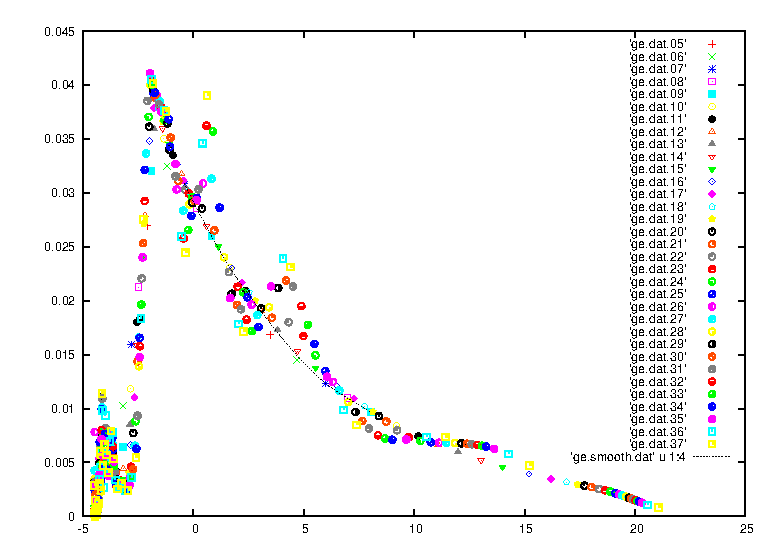
\includegraphics[scale=1.15]{pics/Xe4p_33_gammae.eps}
  \caption{Shifted Stieltjes profile of $\Gamma(E)$ obtained from the
           relativistic FanoADC calculation from
           a 4p$_{3/2}$
           initial state with both $\Gamma$ and $E$ given in atomic units.
           The resonance energy is $E_{res}=0$ and the resulting points
           of the different orders of Stieltjes are plotted separately.
           The smooth curve shows two
           additional peaks related to interactions with Rydberg states as
           discussed in section \ref{section:Stieltjes_profile_properties}.
           }
  \label{figure:Xe4p33_Gamma_profile}
\end{figure}

In case of a 4p$_{3/2}$ initial state, the decay width profile for Stieltjes
orders between 5 and 37 shows a decay
with a threshold at energies below $E_{ref}=0$, which leads to a fairly smooth
curve at the energy of interest.
At higher energies of about \unit[1.5]{a.u.} and
\unit[4.5]{a.u.} additional peaks are observed, which can be explained with
interactions of the initial state description with Rydberg states. These do not
contribute to the decay and hence a smoothing of the total curve neglecting them
is necessary.


\begin{table}[h]
 \centering
 \caption{Auger decay widths of the Xe4p$_{3/2}$ initial states with
          different $M_J$ values and different doubly ionized final
          states.
          All widths are given in \unit{eV}.}
 \begin{tabular}{lcc}
   \toprule
                      & 4p$_{3/2,\pm 3/2}$ & 4p$_{3/2,\pm 1/2}$  \\
   \midrule                                                      
   energy [\unit{eV}] &   147.57           &    147.57          \\
   pole strength       &     0.694          &      0.694         \\
   \midrule                                                     
   $4d^{-2}$          &      --            &        --            \\
   $4d^{-1}5s^{-1}$   & 1.31$\cdot10^{-1}$ & 1.44$\cdot10^{-1}$ \\
   $4d^{-1}5p^{-1}$   & 6.36$\cdot10^{-1}$ & 6.29$\cdot10^{-1}$ \\
   $5s^{-2}$          & 6.27$\cdot10^{-4}$ & 6.29$\cdot10^{-4}$ \\
   $5s^{-1}5p^{-1}$   & 1.50$\cdot10^{-2}$ & 1.49$\cdot10^{-2}$ \\
   $5p^{-1}5p^{-1}$   & 3.21$\cdot10^{-2}$ & 2.90$\cdot10^{-2}$ \\
   \midrule
   total              &   0.814            &   0.818            \\
   \bottomrule
 \end{tabular}
 \label{table:xe_auger_rest}
\end{table}


\begin{table}[]
 \centering
 \caption{Total Auger decay widths of the Xe4p$_{3/2}$ obtained from
          experiment, \ac{MCDF} and this work. All widths are given in \unit{eV}.}
 \begin{tabular}{lcccc}
   \toprule
                        & exp   & calc\footnotemark[1] & calc\footnotemark[2] & calc\footnotemark[3] \\
   \midrule                                                                         
   energy [\unit{eV}]   & 145.6 &  145.0       &  145.0       &   147.57   \\
   $\Gamma$ [\unit{eV}] &  0.54 &  1.80        &  0.3116      &  0.814\\
   \bottomrule
 \end{tabular}
 \label{table:xe_auger_comp}
\end{table}
\footnotetext[1]{\ac{MCDF} calculation excluding final ionic state configuration
                 interaction. \cite{Heinaesmaeki04}}
\footnotetext[2]{\ac{MCDF} calculation including final ionic state configuration
                 interaction. \cite{Heinaesmaeki04}}
\footnotetext[3]{This work.}

The total and partial decay widths for the 4p$_{3/2}$ initial state
are shown in Table \ref{table:xe_auger_rest}. The projection of the
angular total angular momentum of the initial state does not influence
the results, which can be deduced from the almost equal results for the
4p$_{3/2,\pm 3/2}$ and 4p$_{3/2,\pm 1/2}$ initial state. It can easily be seen that
the \ac{CK} processes characterized by the 4d$^{-1}$5s$^{-1}$ and
4d$^{-1}$5p$^{-1}$ final states dominate the decay.

The total decay widths are compared
to experimental values and the results obtained using \ac{MCDF} in
Table \ref{table:xe_auger_comp}. All decay widths are in the order of \unit[1]{eV}.
While the calculation excluding the final ionic state configuration interaction
underestimates
the experimental decay width by \unit[0.23]{eV}, the calculation including the
final ionic state configuration interaction overestimates the experimental value
by \unit[1.26]{eV}. 
The decay width obtained in this work overestimates the experimental decay width
by \unit[0.27]{eV}. 
The FanoADC-Stieltjes approach intrinsically contains configuration interaction
inside the final state subspace. However, only those states characterized by
certain 2h configurations imaging the final state configuration are taken
into account. In contrast to this, in the \ac{MCDF} calculation further hand-picked
satellite contributions are added to the final state description.
Hence, the final state description of the \ac{MCDF} can be more precise
than the one of the FanoADC method.

Considering the large errors of both decay width calculations
their experimental determination, the total decay widths
obtained in this work are in agreement with both the experimental findings and
the other calculations.

\begin{table}[]
  \centering
  \caption{Contributions of the different channels to the total
           decay width for the Auger decay of Xe4p$_{3/2}$ in \%.}
  \begin{tabular}{lccccc}
   \toprule
                   & 4d$^{-1}$5s$^{-1}$ & 4d$^{-1}$5p$^{-1}$ & 5s$^{-2}$ & 5s$^{-1}$5p$^{-1}$ & 5p$^{-2}$ \\
   \midrule
   Ref. \cite{Heinaesmaeki04}\footnotemark[1] & 77.7 & 20.7  &       0.5 &       --           & 1.1     \\
   Ref. \cite{Heinaesmaeki04}\footnotemark[2] & 33.6 & 59.4  &       2.2 &       --           & 4.8     \\
   This work       &      16.1          &       78.1         &    0.1    &     1.8            & 3.9    \\
   \bottomrule
  \end{tabular}
  \label{table:Xe_auger_distr}
\end{table}
%\footnotetext[1]{\ac{MCDF} calculation excluding final ionic state configuration
%                 interaction. \cite{Heinaesmaeki04}}
%\footnotetext[2]{\ac{MCDF} calculation including final ionic state configuration
%                 interaction. \cite{Heinaesmaeki04}}

As discussed in section \ref{section:partial}, the obtained partial decay
widths might suffer from interchannel mixing, which is mainly observed in
the subvalence region. According to this, the intensity distribution
of this work  differs from the ones of reference \cite{Heinaesmaeki04} as
shown in Table \ref{table:Xe_auger_distr}. However, the dominance of the
\ac{CK} process is qualitatively observed in accordance with the other
calculations.


The Xe4p$_{1/2}$ initial state can, as already mentioned, not be described
by a single 1h configuration and therefore, all states with a pole strength
larger than 0.05 and a major contribution of the Xe4p$_{1/2}$ spinor are
investigated. Hereby, also the $4d^{-2}$ configurations are sorted into the
final state subspace in order to take into account a possible \ac{SCK} process.

Figure \ref{figure:Xe4p11_Gamma_profile} shows the decay width profile
of the lowest energy state investigated, which also inhabits the largest
pole strength. It is a well-behaved and smooth curve at energies above $E=0$.
As can easily be seen, the \ac{SCK} decay channel opens directly
in the energy region of interest at $E_{res}=0$. Since the Stieltjes procedure
is not able to produce a clear energy cut at the threshold and the initial state
energies can be expected not to be completely exact due to errors introduced
by the partitioning and additional errors from the ADC(2x) itself, an
unambiguous conclusion, whether the \ac{SCK} channel is open or not,
cannot be drawn.
This decision also determines the choice of which curve of the decay width
profile to choose for the evaluation of the decay width. The results shown
in Table \ref{table:xe_auger_rel11} are the numbers obtained from the
lower curve excluding
the opening channel from the interpolation. In weighing the higher order moments
more than the lower order moments, the decay width would be about twice
as large as the numbers
presented and hence in the order of $\Gamma_{max} \approx \unit[2]{eV}$.

\begin{figure}[]
  \centering
  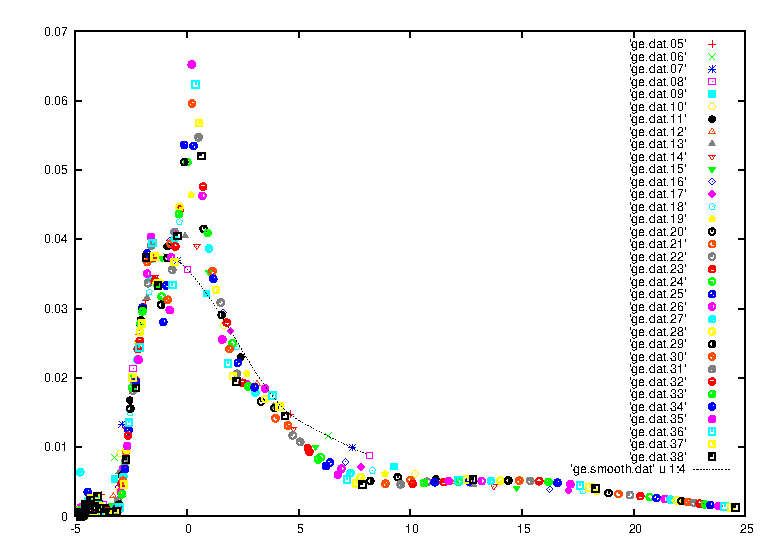
\includegraphics[scale=1.0]{pics/Xe4p_11_gammae.eps}
  \caption{$\Gamma(E)$ of the relativistic FanoADC calculation from a 4p$_{1/2}$
           initial state with both $\Gamma$ and $E$ given in atomic units.
           }
  \label{figure:Xe4p11_Gamma_profile}
\end{figure}


\begin{table}[]
 \centering
 \caption{Auger decay widths of non-negligible satellites with a major
          contribution of the Xe 4p$_{1/2}$. All widths are given in \unit{eV}.}
 \begin{tabular}{lccccc}
   \toprule
   energy [\unit{eV}] & 156.42  & 158.16 & 160.22 & 177.77 & 186.31\\
   pole strength       &   0.332 &   0.093&   0.123&   0.058&   0.068\\
   \midrule
   $4d^{-2}$          & 6.78$\cdot10^{-1}$ & 4.45$\cdot10^{-1}$ & 1.07$\cdot10^{-1}$ & 1.68$\cdot10^{-1}$ & 1.56$\cdot10^{-1}$\\
   $4d^{-1}5s^{-1}$   & 1.34$\cdot10^{-1}$ & 6.93$\cdot10^{-2}$ & 8.61$\cdot10^{-2}$ & 1.12$\cdot10^{-1}$ & 3.39$\cdot10^{-1}$\\
   $4d^{-1}5p^{-1}$   & 2.51$\cdot10^{-1}$ & 9.08$\cdot10^{-2}$ & 1.09$\cdot10^{-1}$ & 1.45$\cdot10^{-1}$ & 3.72$\cdot10^{-1}$\\
   $5s^{-2}$          & 3.10$\cdot10^{-4}$ & 2.21$\cdot10^{-4}$ & 1.91$\cdot10^{-4}$ & 2.12$\cdot10^{-4}$ & 1.81$\cdot10^{-4}$\\
   $5s^{-1}5p^{-1}$   & 3.84$\cdot10^{-3}$ & 1.32$\cdot10^{-3}$ & 2.16$\cdot10^{-3}$ & 1.45$\cdot10^{-3}$ & 8.13$\cdot10^{-3}$\\
   $5p^{-1}5p^{-1}$   & 1.02$\cdot10^{-2}$ & 3.40$\cdot10^{-3}$ & 5.12$\cdot10^{-3}$ & 2.18$\cdot10^{-3}$ & 1.55$\cdot10^{-2}$\\
   \midrule
   total              &   1.077 &   0.610&   0.310&   0.429&   0.891\\
   \bottomrule
 \end{tabular}
 \label{table:xe_auger_rel11}
\end{table}

Even though the FanoADC calculations imply the \ac{SCK} process to have
a large decay width, the calculated value is smaller than the estimated
value of \unit[10--100]{eV} \cite{Heinaesmaeki04}.
I therefore conclude that the broad
feature of the single ionization spectrum in the 4p$_{1/2}$ region is caused
by both the breakdown of the single particle picture with additional fast decay
of all corresponding satellite configurations.


\section{Summary}
From these examples I have shown that the FanoADC-Stieltjes method implemented
in Dirac is able to both reproduce results of the comparable non-relativistic
code of Koloren\v{c}  and results from \ac{MCDF} calculations
including relativistic effects in Auger processes as well as the corresponding
experimental results.
It is to be expected that the relativistic FanoADC-Stieltjes Code is also able
to predict unknown decay widths for larger systems such as dimers and small
clusters, since it is able to treat lower than spherical symmetries.

\section{Character of Energy and Electron Transfer Illustrated Using Pairs and Triples of Atoms}
%\section{Character of Energy and Electron Transfer Illustrated Using Pairs and Triples of Atoms}
\section{Geometric Influence on ICD and ETMD3  Illustrated Using Pairs and Triples of Atoms}
Approximating every system into pairs and triples of atoms is a very useful
first order approximation to both the investigation of energies and
decay widths of a larger system. Pairs and triples are combinations of
two and three atoms, respectively.
These atoms do not necessarily need to form bonds between each other or
even being close, but they are characterized according to fixed internal
coordinates. Each pair and triple can be described by its properties and
is in first order of approximation independent on further, eventually
present, atoms.

In case of the electronic decay processes one is interested in the
energies of the initial $E_{in}$ and the final states $E_{fin}$ of
the corresponding processes. They can be approximated to be

\begin{align}
 E_{in}  &= SIP(X{in}^\beta)\\
 E_{fin} &= SIP(X_{fin1}^\beta) + SIP(X_{fin2}^\beta) + \frac 1d\\
 E_{sec} &= E_{in} - E_{fin}
\end{align}
where $X_{in}$ denotes the initially ionized atom and
$X_{fin1}$ and $X_{fin2}$ describe the two ionized
atoms in the final state. $/beta$ denotes the decay channel characterized
by the total angular momenta of the ionized atoms in the pairs
and triples and $d$ denotes the interatomic distance between the atoms
$X_{fin1}$ and $X_{fin2}$. The initially ionized atom $X_{in}$ can
coincide with one or both of
the final state atoms
$X_{fin1}$ and $X_{fin2}$. As explained in
section \ref{xyz}, the distribution of the vacancies over the different
atoms determine the kind of electronic decay process. Hence, in an
Auger process all three atoms would coincide, for an ICD $X_{in}$
would coincide with one of $X_{fin1}$ and $X_{fin2}$ and for an \ac{ETMD}3
all ionized states are located on different atoms.

In all considered autoionization processes a second electron
is emitted with the kinetic energy $E_{sec}$. If $E_{sec}<0$, then
the final state energy is higher than the initial state energy and the
process is energetically not accessible.

The decay widths of the pairs and triples can be estimated with
different accuracy, but in general, the total decay width $\Gamma$ of
a system is the sum over the decay widths of all channels $\beta$ for
all possible pairs or triples $i$.

\begin{equation}
  \Gamma = \sum\limits_{i,\beta}\Gamma_{i,\beta}
\end{equation}


\subsection{Influence of the Geometry on ICD processes}
\subsubsection{Geometry Dependence of the ICD Energies}

\begin{figure}[h]
 \centering
 \begin{tikzpicture}
    \begin{axis}[domain=4.0:25,
                 samples = 200,
                 xtick={4.0,8.0,...,24},
                 %xticklabels={$-\pi$,$-\frac \pi 2$,0,$\frac \pi 2$,$\pi$},
                 cycle list name = exotic,
                 legend style={anchor= north west},
                 xlabel={$R$ [\AA]},
                 ylabel={$E$ [eV]}
                 ]
      \addplot+[
                mark = none,
                black,
                thick
               ]
               {29.239};
      \addlegendentry{Ar3s$^{-1}$};
      \addplot+[
                mark = none,
                thick
               ]
               {15.7596 + 12.1298 + 14.39964 / x};
      \addlegendentry{Ar3p$_{3/2}^{-1}$Xe5p$_{3/2}^{-1}$};
      \addplot+[
                mark = none,
                thick
               ]
               {15.9371 + 12.1298 + 14.39964 / x};
      \addlegendentry{Ar3p$_{1/2}^{-1}$Xe5p$_{3/2}^{-1}$};
      \addplot+[
                mark = none,
                thick
               ]
               {15.7596 + 13.4363 + 14.39964 / x};
      \addlegendentry{Ar3p$_{3/2}^{-1}$Xe5p$_{1/2}^{-1}$};
      \addplot+[
                mark = none,
                thick
               ]
               {15.9371 + 13.4363 + 14.39964 / x};
      \addlegendentry{Ar3p$_{1/2}^{-1}$Xe5p$_{1/2}^{-1}$};
      \addplot+[
                mark = none,
                thick
               ]
               {15.8188 + 12.5653 + 14.39964 / x};
      \addlegendentry{Ar3p$_{nrel}^{-1}$Xe5p$_{nrel}^{-1}$};
      %\draw[] (axis cs:\pgfkeysvalueof{/pgfplots/xmin},29.239) -- (axis cs:\pgfkeysvalueof{/pgfplots/xmax},29.239);
    \end{axis}
\end{tikzpicture}

 \caption{}
 %\label{}
\end{figure}

\subsubsection{Geometry Dependence of the ICD Decay Widths}

\chapter{ICD and ETMD in Heteroatomar Noble Gas Clusters}
\section{NeAr-Clusters}

\begin{figure}[h]
 \centering
 \begin{tikzpicture}[scale=1.5]

\begin{loglogaxis}[%scale=1.5,
             domain=2:30,
             %y domain=1E-8:10,
             restrict expr to domain={y}{1E-8:15},
             xlabel={R in \AA},
             xtick={2,4,...,10,15,...,25},
             xticklabels={2,4,6,8,10,15,20,25},
             ylabel={$\Gamma(R) in \unit{eV}},
             title={Parameter Fitting of NeNe and NeAr Decay Widths}
             ]

\addplot[only marks,
         mark=x,
         thick,
         diplom4
        ]
        table[
        x expr = \thisrowno{0},
        y expr = \thisrowno{1}
        ]
        {../data/NeAr.dat};
        \addlegendentry{NeAr data};
	
\addplot[
        very thick,
        diplom3,
        samples=200
	]
	{1211057096516.005371 * exp(-11.074016*x) + 23.797274/x^6};
        \addlegendentry{NeAr fit};

\addplot[only marks,
         mark=x,
         thick,
         diplom2
        ]
        table[
        x expr = \thisrowno{0},
        y expr = \thisrowno{1}
        ]
        {../data/Ne2.dat};
        \addlegendentry{Ne$_2$ data};
	
\addplot[
        very thick,
        diplom1
	]
	{19.643762 * exp(-2.789916*x) + 6.204031/x^6};
        \addlegendentry{Ne$_2$ fit};

		
\end{loglogaxis}
\end{tikzpicture}

 \caption{}
 \label{}
\end{figure}

\subsection{Hypothetical, idealized structures of the NeAr clusters}

It is known that small noble gas clusters preferably form icosahedral structures,
while with increasing cluster size a fcc structure becomes more favorable. This transition
occurs at cluster sizes in the range from 750 to 3500 atoms \cite{Martin96,Doye97,Hartke02}.
For our simulations we assume that the clusters of all five experimental cluster sets have 
icosahedric structure. For all sets but set 2 the expansion conditions should result in clusters 
with mean sizes below 750 (see table \ref{table:expansion}). The mean size of the clusters of set 2 is well below 3500.

\begin{figure}[!ht]
 \centering
 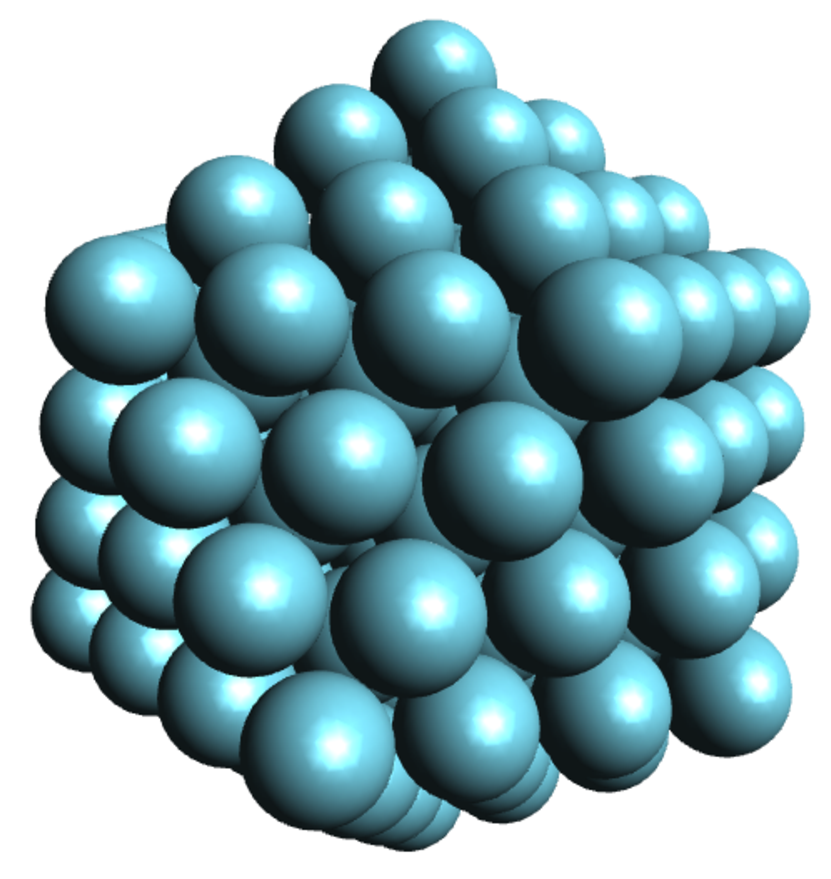
\includegraphics[scale=0.5]{pics/Ar_pure.eps}                        
 \caption{An icosahedral argon cluster with an edge consisting of 
          $c=\unit[4]{atoms}$, containing \unit[147]{atoms},
          distributed over four shells. \unit[55]{atoms} belong
          to the core, 12 are at the vertices, 60 in the edges and 20 inside the
          surfaces.}
 \label{figure:Ar_pure}
\end{figure}    

The actual cluster formation process is understood as follows. First, a three particle
collision has to take place to form argon dimers. Subsequently, single atoms are added to the dimer 
due to collisions. At a later stage these clusters can also collide to form larger clusters. This process,
called coagulation, becomes the dominant process for the formation of very large clusters. 
The experiment of Lundwall et al. \cite{Lundwall07} was interpreted to
show clusters consisting of an argon core with distinct, complete neon
shells around it, which is plausible, since according to the sum of van der Waals
energies, this should be the most stable kind of clusters.
Therefore we take this as a starting point for our considerations of the
average structure of the clusters.

In all structures considered throughout this paper we start from an icosahedral
structure of argon atoms as shown in figure \ref{figure:Ar_pure}.
In this example, it has an edge length
of $c=\unit[4]{atoms}$ and consists of $n_{Ar}=\unit[147]{atoms}$, which can be
calculated as \cite{Martin96}

\begin{equation}
  n_{atoms} = \frac{10}{3} c^3 - 5 c^2 + \frac{11}{3} c -1 .
\end{equation}

For the construction of the structure we assume the minimum
distance between two argon
atoms to be twice the van der Waals
radius of argon $r_{Ar}=$ \unit[1.88]{\AA} \cite{Bondi64}. In order to abide by this
minimum distance in the case of two atoms in a surface position in different
shells, the distance of two atoms in the edges is slightly increased.

As we are going to see in the discussion, the outcome of the experiment
can not completely be explained by an argon core surrounded by complete neon shells.
This leads us to consider other structures with an argon core somehow surrounded
by neon atoms. These we divide into three types, so that, in total, we have four
different classes of cluster structures as shown in figure \ref{figure:structures}:

\begin{enumerate}
 \item complete shells
 \item incomplete shells around complete shells
 \item caps
 \item randomly arranged neon atoms around complete shells
\end{enumerate}

\begin{figure}[!h]
 \centering
 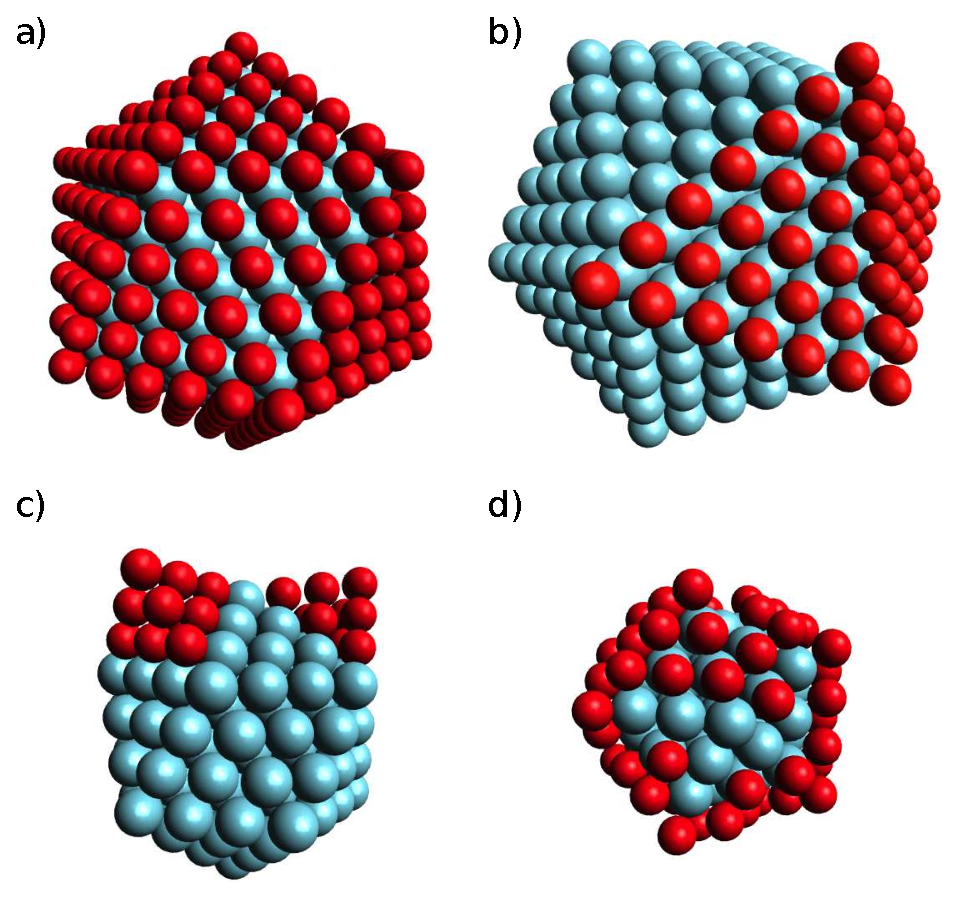
\includegraphics[scale=0.9]{pics/NeAr_structures1.eps}
 \caption{Structure classes considered in our calculations.\\
          a) complete shells, in this example $c=\unit[5]{atoms}$ with one layer
          neon atoms,\\
          b) incomplete shells, in this example
          $c=\unit[6]{atoms}$ with two covered trinangular surfaces
          of neon,\\
          c) caps, in this example $c=\unit[4]{atoms}$ with two caps,\\
          d) randomly arranged neon atoms around a full shell cluster,
          here $c=\unit[3]{atoms}$ directly covered by neon atoms
          with an argon content of \unit[47]{\%}.}
 \label{figure:structures}
\end{figure}

In the case of an argon cluster with one or more complete shells of neon
atoms around it, first the core structure is created and afterwards the
outer shells are constructed around it, such that the minimum distance between a
neon atom in the surface and an argon atom in the shell beneath is the sum
over the van der Waals radii, where $r_{Ne}=$\unit[1.54]{\AA} \cite{Bondi64}
(see figure \ref{figure:structures} panel a).

Not all experimentally determined argon contents in the mixed clusters
fit to complete neon shells. Maintaining the idea of shells,
we consider the possibility of incomplete shells.
The cluster structures are created analogously to the
complete shells except that not all triangular surfaces areas of the argon core
are covered by neon atoms (for an example see figure \ref{figure:structures}
panel b).

Another possibility are caps covering surface areas as shown
in figure \ref{figure:structures} panel c. These structural elements
do not exhibit minimum energy for clusters, but they might explain a
large number of neon-neon interactions compared to the number of
neon-argon interactions in the experiments.
The neon-neon distances within the caps are
calculated in the same
manner as described before for the (in-)complete shells.
A whole manifold of different positionings of several caps are in principle
possible, but in our calculations we were able to see, that these different
placements of caps did not change the ratios of NeAr to NeNe ICD for a
constant number of caps. Since we
are unable to distinguish these structures, we will limit ourselves to the
discussion of structures containing different numbers of caps.

One could also think about neon atoms randomly arranged around a homonuclear
or heteronuclear cluster with complete shells and randomly attached neon
atoms around it as shown in figure \ref{figure:structures} panel d.
It is constructed as a cluster with complete shells and afterwards adding
neon atoms in random positions of the next layer until the requested
$n_{Ar}/n_{Ne}$ ratio is reached.

All these structures are idealized and highly symmetric, which reduces
the computational cost. Vibrations inside the clusters will change the atom
distances and hence both the kinetic energy of the ICD electron as well as
the decay widths. As has been shown for NeAr \cite{Scheit06}, the ICD processes
are faster than dynamical rearrangements, caused by Coulombic attraction
after the initiating ionization, or vibrations. In case of the neon dimer, the
ICD lifetime is of comparable size to the rearrangement time and hence
influences the ICD electron spectra /cite{Scheit03}. However, in clusters, the
initially ionized atom interacts with more than one other atom, which leads
to more neighbors it can undergo ICD with and hence the decay width increases
to first approximation linearly with the number of nearest neighbors.
At the same time, the larger number of neighbors stabilizes the position
of the initially ionized atom in space compared to the dimer.
Therefore we will assume that the structures given above are good
approximations to the decaying clusters.




\subsection{Interpretation of the graphs}

In order to have comparable numbers we choose the argon content within
the clusters and the amount of NeAr-ICD compared to the total ICD to
characterize every measurement and theoretical calculation.
Throughout the paper, including the supplementary material, we stick to the same 
colour coding as for the experimental spectra shown in figure \ref{figure:selected_ICD_specs},
for which the numbers are listed in table \ref{table:clustervalues}.
The results are going to be plotted as in figure \ref{figure:incompl01_02_explain}.
As an example we show cluster of the class of an incompletely filled neon shell
around an argon core with a an edge size of $c=2$
surrounded by one complete shell of neon atoms.
Here the ratio of NeArICD to total ICD is plotted against the argon content
of the cluster. The results of the five different experimental conditions and their
errors are shown by the coloured areas, where the colour corresponds to the
set with the same colour as in figure \ref{figure:selected_ICD_specs}.
They are going to be the same in all plots throughout the paper.
Additionally plotted are the theoretical results for the different structures
parted into first the classes of the structures and secondly by the size of the argon core.
The higher the argon content is, the less of the 20 surfaces of the underlying
complete shell is covered by either layer(s) or caps. The easiest way to interpret
the graphs is to start from a complete shell and then covering one surface. This
corresponds to the rightmost theoretical value within a group. Each step further
to the left refers then to one more covered layer with either caps or layers.\\

\begin{figure}[!h]
  \centering
  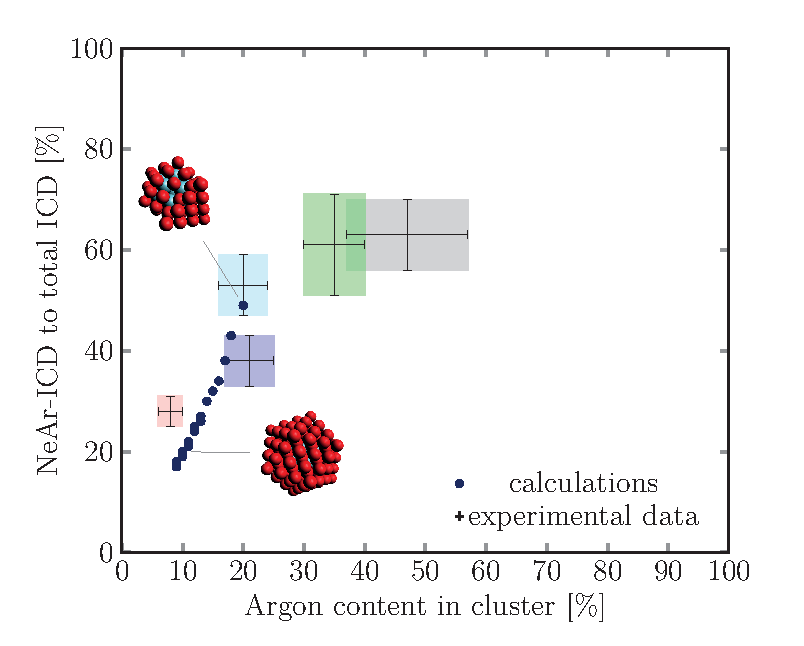
\includegraphics[scale=0.75]{pics/incompl01_02_mit_inlays.eps}
  \caption{NeArICD to total ICD ratio plotted against the argon content
           in the cluster for both experimental results for all five sets of
           conditions as well as theoretical calculations for cluster structures
           with an incomplete outermost shell surrounding an argon core of
           $c=2$ and one additional complete neon shell. For illustration, pictures
					of two structures are included at their respective theoretical values.}
  \label{figure:incompl01_02_explain}
\end{figure}

By looking for agreements of theoretical and experimental values we deduce
possible structures.
The agreement between experimental and theoretical results are evaluated
using the graphical distance from the experimental results
\begin{equation}
  d = \sqrt{\Delta_{Ar}^2 + \Delta_{\Gamma}^2}    ,
\end{equation}
where $\Delta_{Ar}$ and $\Delta_{\Gamma}$ denote the deviation of the argon content
and the ratio of NeArICD decay width and the total decay width, respectively.
Only such structures are considered, where the argon content of the model
structure lies within the error range of the experimental findings.


\subsection{Assignment of the different measurements to cluster structures}
For our assignments we use the following criteria:

\begin{itemize}
 \item onsets of single ionization potentials for the determination
       of the size of the argon core
 \item positions of NeAr-ICD peak
 \item relative expected mean cluster sizes (see table \ref{table:expansion})
 \item agreement of predicted and measured ICD (see table \ref{table:assignments})
\end{itemize}

From the onsets of the single ionization potentials and the position of the
NeAr-ICD peak at a lower energy we deduce that the mean argon core of set 5
is the smallest of all measured ensembles. Since the nearest neighbours have
the largest influence of such a shift we interprete these clusters to have
an edge length of either $c=1$ or $c=2$.\\
Since the estimation of mean cluster sizes based on Hagena refer to expansions
of only one atom type, only the results with the same argon content should
be compared. From this we expect the core of set 2 to be bigger than the core
of set 4 and the core of set 3 to be slightly larger than the core of set 1.
These estimations do not have to resemble the final conclusions, since the
approach is only valid for homogeneous clusters, but can give hints
in the following procedure. The assignment due to geometrical distance
of the predicted results from the experimental counterparts is to be found in
table \ref{table:assignments}. There best results for all sets are shown
in the following way: $c$ depicts the number of atoms in the longest edge
of the argon core, which is then covered by a number of additional complete
neon shells with additional covered triangular surfaces or randomly arranged atoms
and $d$ denotes the geometrical distance.\\

\begin{table}[!h]
  \caption{Note that for set 4 only the random arrangement is listed,
           for which the argon content exactly equals the experimental one.}
  \centering
  \begin{tabular}{lccccc}
    \toprule
     Set  & $c$ & complete Ne shells & covered surfaces & random & $d$\\
    \midrule
      1   & 4   &          1         &        1         &   -    & 2.000\\
      1   & 5   &          1         &        2         &   -    & 4.472\\
      1   & 2   &          0         &        5         &   -    & 4.472\\
    \midrule
      2   & 3   &          1         &        -         &   x    & 1.000\\
      2   & 3   &          1         &        1         &   -    & 3.162\\
      2   & 2   &          0         &        8         &   -    & 4.123\\
    \midrule
      3   & 2   &          1         &        3         &   -    & 4.000\\
      3   & 3   &          1         &        7         &   -    & 4.123\\
      3   & 3   &          1         &        8         &   -    & 4.472\\
    \midrule
      4   & 2   &          1         &        -         &   x    & 2.000\\
      4   & 2   &          1         &        1         &   -    & 4.000\\
    \midrule
      5   & 2   &          1         &       13         &   -    & 8.246\\
      5   & 2   &          1         &       14         &   -    & 9.220\\
      5   & 2   &          1         &       15         &   -    & 9.220\\
    \bottomrule
  \end{tabular}
  \label{table:assignments}
\end{table}

We are going to discuss the structure assignment in descending order
of the set number, which more or less corresponds to a discussion with
increasing size of the clusters.\\
We start our assignment with set 5 (red). As already mentioned we expect these clusters
to be small and, additionally, the smallest ones measured. These expectations are
in agreement with the results of figure \ref{figure:incompl01_02_explain}
(also to be found in the
appendix in figure \ref{incompl01_02}), where the red square
can be matched with a cluster with an argon core with $c=2$, one complete
shell of neon atoms 
and one almost complete
shell with 13 -- 20 out of 20 surfaces covered by neon atoms. None of the
theoretical estimates coincide with the experimental findings. This might be
explained by even smaller clusters not showing an icosahedral argon core, but
a coagulation of 2--11 atoms plus some neon atoms.

Set 4 (turquoise) shows a very good agreement for a structure with $c=2$ with one
complete shell of neon atoms and some additional atoms (see figures
\ref{random02} and \ref{incompl01_02} or in the example above). Whether these atoms are
randomly arranged around the complete shells or are to be found together can not
finally be decided. From the geometric distance, the random arrangement should
be preferred.

The results of set 3 (blue) shows a good agreement with structures
of $c=2$ or $c=3$ surrounded by one complete shell of neon atoms and additional
neon atoms covering 3 or 7 -- 8 triangular surfaces, respectively 
as shown in figure \ref{incompl01_02} and \ref{incompl01_03}. 

With the two latter assignments we are able to distinguish
the structures of two cluster manifolds with the same argon content by utilizing the
ICD spectra.

Set 2 (green) can be assigned to core sizes of $c=2-3$ plus further neon atoms
(see figures \ref{incompl00_02} and \ref{incompl01_03}).
In the case of $c=3$ one additional complete shell of neon atoms fits
best to the experimental results, but as for set 4 the arrangement as such for
some few additional atoms can either be random or coagulated.
In case of $c=2$ the best fit holds for no additional complete shell of
neon atoms but with 8 triangular surfaces covered, the shell is almost halfway filled.
Further structures with larger core sizes as $c=4$
are also quite probable. Considering, that 
both from Hagena's approach and considering the single ionization potential
onsets of the Ar3p band, set 2 is supposed to have the largest mean structure
core. These structures might be closer to reality than the ones of the small clusters
with $c=2,3$.

Due to the large error bars, set 1 (black) can be assigned to a whole manifold
of different structures with $c = 2 - 6$ within the error bars
either with caps or, more probably,
with about one complete shell of neon atoms, plus maybe additional covered surfaces
or randomly surrounded by neon atoms. Since caps should be energetically less
favourable than the other structures, we suspend those structures and concentrate
on the rest.
From Hagena's approach we concluded, that the core of the clusters of set 1
should be slightly
smaller or of comparable size as the clusters from set 3. Therefore we assume
the average cluster structure to consist of an argon core of $c=2-4$ shells
with one complete neon shell and possibly one further incomplete shell, of
which we can't give more detailed information.

We may have to consider completely different structures not investigated in this
paper. It might be, that formed mixed clusters collide and coagulate, yielding
structures impossible to be estimated by a core-shell structure of the kinds
presented in this paper. 

From the best agreement of the calculated NeArICD to total ICD ratios listed in table
\ref{table:assignments}, we plot the corresponding estimated spectra in figure
\ref{figure:theo_specs} folded by gaussians with a width of \unit[250]{meV}.
From these spectra and the underlying calculations
we conclude, that the shoulders of both the NeNeICD and the NeArICD peak
at \unit[2.5--4]{eV} and \unit[8--10]{eV}
correspond to next-nearest neighbours inside the clusters, while the differences
in the main peak stem from almost equal atomic distances but different positions
in the cluster such as corner, edge or surface.\\
The main peaks of the NeNeICD correspond well with the experimental observations
of figure \ref{figure:selected_ICD_specs}.\\
The onset of the NeArICD peak depends on the shielding of the argon atom
and hence the cluster size. For set 5 the assignment seems to be correct, while
for set 4, the experiment shows a higher energy of the ICD electron. 

---> den satz versteh ich nicht ganz:
This change does not need to be physical as we in the beginning assumed clusters
until $c=2$ to have the higher mean ionization potentials. 
----

The truth, however,is not a spontaneous jump from one shell to the other, but rather a decrease
with more and more atoms. If one is interested in clusters of $c\le2$ only, one
should take care of a more detailed description of the different ionization
potentials for different cluster sites.\\

\begin{figure}[!ht]
  \centering
  \input{pics/near_clusters/spec-250meV}
  \caption{Calculated ICD electron spectra for those structures given in table
           \ref{table:assignments} with the best agreement to the experimental
           argon content and NeArICD to total ICD ratio. The intensities are given
           in arbitrary units and are normalized to the peak height of the NeArICD
           peak and the spectra are folded by Gaussians with widths of \unit[250]{meV}.
           The theoretically calculated specrta nicely match the experimental ones in figure
           \ref{figure:selected_ICD_specs}.
           Both, the NeNeICD peak at low energies and the NeArICD peak
           at higher kinetic energies, show a peak structure which can be related
           to different distances of the atoms involved in the process within the
           clusters. For more details, see the text.}
  \label{figure:theo_specs}
\end{figure}


\section{ArXe-Clusters}

\begin{figure}[h]
 \centering
 \begin{tikzpicture}
    \begin{axis}[domain=4.0:25,
                 samples = 200,
                 xtick={4.0,8.0,...,24},
                 %xticklabels={$-\pi$,$-\frac \pi 2$,0,$\frac \pi 2$,$\pi$},
                 cycle list name = exotic,
                 legend style={anchor= north west},
                 xlabel={$R$ [\AA]},
                 ylabel={$E$ [eV]}
                 ]
      \addplot+[
                mark = none,
                black,
                thick
               ]
               {29.239 - 0.636};
      \addlegendentry{Ar3s$^{-1}$};
      \addplot+[
                mark = none,
                thick
               ]
               {15.7596 - 1.0 + 12.1298 - 1.3 + 14.39964 / x};
      \addlegendentry{Ar3p$_{3/2}^{-1}$Xe5p$_{3/2}^{-1}$};
      \addplot+[
                mark = none,
                thick
               ]
               {15.9371 - 0.4 + 12.1298 -1.3 + 14.39964 / x};
      \addlegendentry{Ar3p$_{1/2}^{-1}$Xe5p$_{3/2}^{-1}$};
      \addplot+[
                mark = none,
                thick
               ]
               {15.7596 - 1.0 + 13.4363 -0.9 + 14.39964 / x};
      \addlegendentry{Ar3p$_{3/2}^{-1}$Xe5p$_{1/2}^{-1}$};
      \addplot+[
                mark = none,
                thick
               ]
               {15.9371 -0.4 + 13.4363 - 0.9 + 14.39964 / x};
      \addlegendentry{Ar3p$_{1/2}^{-1}$Xe5p$_{1/2}^{-1}$};
      \addplot+[
                mark = none,
                thick
               ]
               {15.8188 - 0.8 + 12.5653 - 1.17 + 14.39964 / x};
      \addlegendentry{Ar3p$_{nrel}^{-1}$Xe5p$_{nrel}^{-1}$};
      %\draw[] (axis cs:\pgfkeysvalueof{/pgfplots/xmin},29.239) -- (axis cs:\pgfkeysvalueof{/pgfplots/xmax},29.239);
    \end{axis}
\end{tikzpicture}

 \caption{}
 %\label{}
\end{figure}



\chapter{Summary and Outlook}

In this thesis, the importance of relativstic effects on autoionization
processes, especially \ac{ICD}-like
processes, and cluster environments have been discussed.
For this purpose, asymptotic expressions for the relativistic decay width of the ICD
and both, relativistic and non-relativstic asymptotic expressions for the ETMD3
have been derived. Additionally, the non-relativistically known
FanoADC-Stieltjes approach
using a partitioning of the Hamiltonian by 2h configurations has been implemented
in the relativistic programme package \verb|DIRAC| \cite{DIRAC13},
which allows for the
description of decay width including relativistic effects.
In order to model the experimental secondary electron spectra of noble gas
clusters, the model of pairs and triples was introduced and automatized in the
programme \verb|HARDRoC| \cite{HARDRoC}. It enables the estimation of
decay widths of the total system from data of the compounds.

In the studies of the atomic Auger process, scalar-relativistic effects were
found to increase the decay width compared to the non-relativistic results
due to larger orbital overlaps of the initial and final states. Especially
in ETMD processes, whose decay width is governed by the orbital overlap
of the two units involved in the energy transfer, similiar significant
decay width influences might be observed.

Throughout all systems containing heavy elements, the spin-orbit coupling
shows a pronounced effect on the secondary electron spectrum by increasing the
number of possible channels and hence, the number of peaks. This feature cannot
be explained using a non-relativistic methodology.
If the decay channels are close to threshold, this energetic splitting
can cause a non-relativistically closed decay channel to be partly open. On
the other hand, not all relativistic channels corresponding to one specific
open non-relativistic channel need to be open.

Additionally, geometry has a great impact on the opening and closing of channels
in \ac{ICD}-like processes. The closer the atoms ionized in the final state are,
the lower is the kinetic energy of the secondary electron and the channel
closes at some internuclear distance.

In clusters, the additional effect of charge stabilization shifts the secondary
electron as well. These shifts are treated by using experimentally obtained
ionization energies for exactly the same experimental conditions as for the
secondary electron spectra.
Furthermore, statistical effects were found to increase the decay width
for both the ICD and the ETMD. Since the ICD decay width scales with the number
of nearest neighbours and the ETMD3 decay width scales with the number of nearest
neighbours squared, the ETMD3 is statistically preferred and can therefore compete
with the usually faster ICD.

Based on the strong structure dependence of the secondary electron spectrum
observed during the PhD, a new
structure analysis method for noble gas clusters was developed. If two
competing ICD-like processes are energetically accessible and can be measured
independently, the comparison of the experimentally obtained cluster
composition and relative peak intensities can be compared to theoretically
modelled spectra for a large variety of structures. From the best agreement,
the mean cluster structure can be deduced as was carried out for
a set of experimentally created NeAr cluster manifolds.

In the future, it would be worth investigating \ac{ICD} processes with electron
transitions forbidden in the non-relativistic description.
Additionally, the ETMD3 process should be investigated using the relativistic
FanoADC-Stieltjes approach studying the scalar-relativistic effects observed
for the case of the Auger effect following an ionization of the Xe4d.

It might be worth implementing the FanoADC based on an energy partitioning in
order to obtain partial decay width for the separate final states and to
improve their accuracy.

For the estimation of secondary electron spectra of clusters,
the investigation of clusters with more complex
constituents than noble gas atoms without spherical symmetry,
e.g., water molecules, would be a challenging task.

\include{outlook}

\begin{appendix}

\chapter{Mathematical Appendix}
\section{Cauchy distribution} \label{section:app_cauchy}
The Cauchy distribution is a continuous probability distribution
with the probability density function

\begin{equation}
  f(x;x_0,\gamma) = \frac 1\pi \frac{\gamma}{(x-x_0)^2 + \gamma^2}
\end{equation}
where $x_0$ denotes the location parameter of the peak and
$2 \gamma$ is the full width half maximum (FWHM).\\
Its height or amplitude is $A = \frac{1}{\pi\gamma}$.
In most cases the
Cauchy distribution is normalized to 1. However, it is easy to show,
that $\gamma$ is completely
independent of the normalization and more generally of any prefactor
as long as the structure of the denominator is conserved.
Other names of the Cauchy distribution are Lorentz distribution or
Lorentzian function.


\begin{figure}[h]
  \centering
  \input{pics/cauchy_pgf}
  \caption{Probability density function of a Cauchy distribution with a
           maximum at $x_0$ with a height of $A=\frac{1}{\pi\gamma}$.}
  \label{figure:cauchy_distribution}
\end{figure}


In physics very often the following three parameter Lorentzian function

\begin{equation}
  f(x;x_0,\gamma,A) = A \frac{\gamma^2}{(x-x_0)^2 + \gamma^2}
\end{equation}
is used. As stated above and easily to show, this reformulation does
not effect the value of the FWHM $2 \gamma$.



\chapter{Properties of Noble Gas Atoms}

\begin{table}[h]
 \caption{Atomic ionization energies, lifetimes and relative ionization
          cross sections.}
 \centering
 \begin{tabular}{lcccccc}
  \bottomrule
     & $SIP(np_{3/2})$    & $SIP(np_{1/2})$    & $SIP(ns_{1/2})$    & $\tau(ns_{1/2})$ & $\chi=\frac{\tau_{1/2}}{\tau_{3/2}}$ & $\frac{\sigma_{3/2}}{\sigma_{1/2}}$ \\
  \midrule
   Ne& \unit[21.5645]{eV} & \unit[21.6613]{eV} & \unit[48.475]{eV} & \unit[1.429]{ns} & 2.04 & 2.0 \\
   Ar& \unit[15.7596]{eV} & \unit[15.9371]{eV} & \unit[29.239]{eV} & \unit[4.684]{ns} & 2.05 & 1.875\\
   Xe& \unit[12.1298]{eV} & \unit[13.4363]{eV} & \unit[xx.yyyy]{eV} & \unit[]{ns} &   & 1.6  \\
  \midrule
   Ne$_{nrel}$ & \multicolumn{2}{c}{\unit[21.5968]{eV}} & \unit[48.475]{eV} & \unit[1.429]{ns} & -- & --\\
   Ar$_{nrel}$ & \multicolumn{2}{c}{\unit[15.8188]{eV}} & \unit[29.239]{eV} & \unit[4.684]{ns} & -- & --\\
   Xe$_{nrel}$ & \multicolumn{2}{c}{\unit[12.5652]{eV}} & \unit[xx.yyyy]{eV} & \unit[]{ns} & -- & --  \\
  \bottomrule
 \end{tabular}
 \label{table:noble_atom_properties}
\end{table}

\begin{table}[h]
 \caption{Shift of atomic ionization energies due to a cluster environment.
          All values are given in eV.}
 \centering
 \begin{tabular}{lcccccc}
  \toprule
       & \multicolumn{2}{c}{$\Delta(np_{3/2})$} & \multicolumn{2}{c}{$\Delta(np_{1/2})$} & \multicolumn{2}{c}{$\Delta(ns_{1/2})$} \\
       & bulk    & surface & bulk    & surface & bulk    & surface \\
  \midrule
   Ne  &         &         &         &         &         &         \\
   Ar  &         &         &         &         &         &         \\
   Xe  &         &         &         &         &         &         \\
  \bottomrule
 \end{tabular}
 \label{table:cluster_shifts}
\end{table}







\chapter{NeAr Cluster Structure Agreement Plots}
%\section{Complete Shells}
\begin{figure}[h]
    \centering
    \input{pics/near_clusters/schale02}
    \caption{Complete neon shells with $c=2$.}
    \label{compl02}
\end{figure}

\begin{figure}
    \centering
    \input{pics/near_clusters/schale03}
    \caption{Complete neon shells with $c=3$.}
    \label{compl03}
\end{figure}

\begin{figure}[h]
    \centering
    \input{pics/near_clusters/schale04}
    \caption{Complete neon shells with $c=4$.}
    \label{compl04}
\end{figure}

%\clearpage


%\section{Incomplete Shells Surrounding Complete Shells}
%\subsection{No Complete Neon Shells}
\begin{figure}[h]
    \centering
    \input{pics/near_clusters/in-shell00-core02}
    \caption{Incomplete shells with $c=2$ and no complete neon shell.}
    \label{incompl00-core02}
\end{figure}


%\subsection{One Complete Neon Shell}
\begin{figure}[h]
    \centering
    \input{pics/near_clusters/in-shell01-core02}
    \caption{Incomplete shells with $c=2$ and one complete neon shell.}
    \label{incompl01-core02}
\end{figure}

\begin{figure}
    \centering
    \input{pics/near_clusters/in-shell01-core03}
    \caption{Incomplete shells with $c=3$ and one complete neon shell.}
    \label{incompl01-core03}
\end{figure}

\begin{figure}[h]
    \centering
    \input{pics/near_clusters/in-shell01-core04}
    \caption{Incomplete shells with $c=4$ and one complete neon shell.}
    \label{incompl00-core01}
\end{figure}

\begin{figure}
    \centering
    \input{pics/near_clusters/in-shell01-core05}
    \caption{Incomplete shells with $c=5$ and one complete neon shell.}
    \label{incompl01-core05}
\end{figure}

%\clearpage


%\section{Randomly Arranged Neon Atoms around Complete Shells}
\begin{figure}[h]
    \centering
    \input{pics/near_clusters/random-core02}
    \caption{Random arrangements with $c=2$.}
    \label{random-core02}
\end{figure}

\begin{figure}
    \centering
    \input{pics/near_clusters/random-core03}
    \caption{Random arrangements with $c=3$.}
    \label{random-core03}
\end{figure}

\begin{figure}[h]
    \centering
    \input{pics/near_clusters/random-core04}
    \caption{Random arrangements with $c=4$.}
    \label{random-core04}
\end{figure}


%Programmes
\chapter{Programmes and Scripts}

\section{HARDRoC --- Hunting Asymptotic Relativistic Decay Rates of Clusters}
\section{Relativistic FanoADC}
\section{\textsc{icoclus}}

Icoclus is a selection of python scripts creating xyz-coordinate
files for idealized heteronuclear clusters with a basic
icosahedral structure.
All structures contain an icosahedral core of one atom type
surrounded by atoms of the second atom type in different ways.
Hereby it has to be mentioned, that these cluster structures are not
energetically optimized but build using the scientific guess
that the atomic distances of each pair of atoms in the clusters
can be described as the sum of the van-der-Waals
radii.

The newest version is currently available in a git repository in the local
network of the Theoretical Chemistry group at the university of
Heidelberg and can be cloned via
\begin{verbatim}
 git clone /home/elke/pub/icoclus 
\end{verbatim}


\subsection{Construction of the Core Icosahedral Cluster}
The vertex coordinates of a regular icosahedron are given by

\begin{align}
  \left(  0 , \pm \frac a2 ,  \pm\frac a2 \varphi \right) \nonumber\\
  \left(  \pm\frac a2 , \pm \frac a2 \varphi ,  0 \right) \nonumber\\
  \left(  \pm \frac a2 \varphi , 0 ,  \pm\frac a2 \right)
\end{align}
where $a$ describes both the distance from the center to each vertex
and the length of an edge and $\varphi = \frac 12 (1+\sqrt{5})$.

Icosahedral clusters are build of different shells, each of them
characterized by the number of atoms per edge $c$. Starting from a
central atom, a shell with $c=2$ is added, afterwards one with $c=3$
and so on, until the desired cluster size is achieved.
$a$ is determined by the approriate sum over v. d. Waals radii.

Here one needs to consider, that in these packed icosahedral shells
the distance between the closest atoms within one shell is
larger than the closest distance of two atoms of neighbouring shells.
In order to achieve the overall minimum distance between two atoms
to be the sum of their van-der-Waals radii, we scale our vertex
distance $a$ such, that the distance between the surfaces is given by
the sum of the v. d. Waals radii.

\begin{equation}
 a' = a \frac{2}{\sqrt{1+\varphi^2}}
\end{equation}

In each shell first the vertex atoms are created and then corresponding
to the size of the shell atoms in the edges and in the end the atoms
lying in the surfaces.

\subsection{Complete Shells}
Around the icosahedral core cluster more complete shells consisting
of the second atom type are constructed. Hereby the distance between
the central atom and the vertices is calculated as the sum over the
contributing v. d. Waals radii. and scaled as in the case of the core
vertices.

\subsubsection{Manual of \lstinline|icoclus.py|}
In the header of the script \lstinline|icoclus.py| the following
controlling variables are defined.

\begin{lstlisting}
##################Input Variables ##################################
   atcore  = 'Ar' # atomtype of the core atoms
   atouter = 'Ne' # atomtype of the outer shells
   
   rcore =  1.88  # radius of core atoms
   router = 1.54  # radius of outer shell atoms
   
   n_core = 1     # number of atoms in the longest edge
   #n_outer = raw_input('How many layers of atoms do you want to have? ')
   #n_outer = int(n_outer)
   n_outer = 1    # number of additional shells
\end{lstlisting}

These are to be adjusted according to the desired structure.
Afterwards the script is run from the terminal.
The two commented lines are convenient if several cluster structures
of the same type but with different numbers of second atom type shells.
In this case the two commented lines need to be uncommented and the last
line to be commented out.

\subsection{Incomplete Shells}
It is also possible to generate incomplete shells around a core and
eventually complete shells of the second atom type.

\subsubsection{Manual of \lstinline|incompl_shells.py|}
In the header of \lstinline|incompl_shells.py| the following section
with the
input variables is to be found.

\begin{lstlisting}
##################Input Variables ##################################
   atcore  = 'Ar' # atomtype of the core atoms
   atouter = 'Ne' # atomtype of the outer shells
   
   rcore   = 1.88 # radius of core atoms
   router  = 1.54 # radius of outer shell atoms
   
   n_core  = 1    # number of atoms for the longest edge
   n_sec   = 2    # number of complete layers of the second atom type
   n_outer = 1    # do not change
   
   #no_surfaces = 3 + 1
   no_surfaces = raw_input('How many surfaces do you want to be covered? ')
   no_surfaces = int(no_surfaces)
\end{lstlisting}
Here \lstinline|n_outer| declares the number of shells being
partially filled. Changing it results in a different cluster class.
A nicer way to accomplish structures of this other class is to use the
script \lstinline|area_ico.py|.\\
It is important to notice, that the script is going to fail,
if the number of covered triangular surfaces is 0. In the case of
no additional incomplete shells covered being the desired structure,
one should consider using icoclus.py.


\subsection{Triangular Surfaces Covered by Layers of Atoms}
One might consider triangular surfaces covered by several layers of
atoms of the second atom type, hereby creating subsets of complete
shells as shown in figure \ref{}.

\subsubsection{Manual of \lstinline|area_ico.py|}
In the header of \lstinline|area_ico.py| the following control section
is found with the variables to be adjusted.

\begin{lstlisting}
##################Input Variables ##################################
   atcore  = 'Ar' # atomtype of the core atoms
   atouter = 'Ne' # atomtype of the outer shells
   
   rcore   =  1.88  # radius of core atoms
   router  = 1.54  # radius of outer shell atoms
   
   n_core  = 3     #number of atoms for the longest edge
   n_outer = raw_input('How many layers of atoms do you want to have? ')
   n_outer = int(n_outer)
   #n_outer = 1   # number of layers on top of the selected surfaces
   
   no_surfaces = 5 + 1 # number of triangular surfaces covered
\end{lstlisting}


\subsection{Caps}
One might think of a structure as shown in figure \ref{}, where the
surfaces of the core cluster are covered with caps.

In contrast to the incomplete shells here one might consider both different
numbers of caps as well as multiple arrangements of the caps on the surfaces.
Within the script the 20 surfaces are numbered and hence a manifold of
combination of structures for a given number of caps is possible.
Since the calculation of all different combinations is tedious
it is beneficial to be able to know which of these combinations are symmetry
equivalent. This information can be obtained with the help of the script
\lstinline|stat_caps.py|. For a given number of caps it prints for each
symmetry equivalent structures of one combination of capped surfaces
and the number of possible realizations of it. Afterwards the structures
can be constructed with \lstinline|scatter_cap_ico.py|.

\subsubsection{Manual of \lstinline|stat_caps.py|}
\begin{lstlisting}
##################Input Variables ##################################
   atcore  = 'Ar' # atomtype of the core atoms
   atouter = 'Ne' # atomtype of the outer shells
   
   rcore   = 1.88 # radius of core atoms
   router  = 1.54 # radius of outer shell atoms
   
   n_core  = 2    #number of atoms for the longest edge
   n_outer = n_core - 1 # do not change
   
   n_caps  = 2    # number of caps
\end{lstlisting}
The only number to be adjusted is \lstinline|n_caps|, all other variables
do not influence the result.


\subsubsection{Manual of \lstinline|scatter_cap_ico.py|}
\begin{lstlisting}
##################Input Variables ##################################
   atcore  = 'Ar' # atomtype of the core atoms
   atouter = 'Ne' # atomtype of the outer shells
   
   rcore   = 1.88 # radius of core atoms
   router  = 1.54 # radius of outer shell atoms
   
   n_core  = 4    #number of atoms for the longest edge
   #n_core = raw_input('How many core layers do you want to have? ')
   #n_core = int(n_core)
   n_outer = n_core - 1 # do not change
   
   caps   = [1,5]
   n_caps = len(caps)
\end{lstlisting}
\lstinline|caps| is a python list and here the combination of surface
numbers obtained from \lstinline|stat_caps.py| is to be entered.



\subsection{Randomly Arranged Atoms Around Complete Shells}
For a given ratio between the number of core and the number of surrounding
atoms one can create structures with a fixed icosahedral cluster of closed
shells and atoms
of the second type randomly arranged in the next shell until the desired
ratio is obtained.
In the script \lstinline|random_ico.py| the structures are not created
by adding atoms randomly to the outermost shell but by constructing the
shell, shuffling the order of atoms in this shell using python's random
functionality based on the Mersenne Twister method \cite{python_random,Matsumoto98}
and then deleting as many
atoms as necessary to achieve the desired ratio. 

\subsubsection{Manual of \lstinline|random_ico.py|}
\begin{lstlisting}
##################Input Variables ##################################
   atcore  = 'Ar'   # atomtype of the core atoms
   atouter = 'O'    # atomtype of the outer shells
   
   rcore   = 1.88   # radius of core atoms
   router  = 1.54   # radius of outer shell atoms
   
   n_core  = 5      # number of atoms for the longest edge
   n_sec   = 0      # number of complete shells of second atom type
   ratio   = 3.8868 # nc_atoms/no_atoms
   
   n_outer = 1      # do not change
\end{lstlisting}


\section{\textsc{fccclus}}
\section{Utilities}


\end{appendix}


\bibliographystyle{jcpsty_deutsch}
\bibliography{theolit}

\end{document}
